% !TEX TS-program = pdflatex
% !TEX encoding = UTF-8 Unicode
\documentclass[a4paper,11pt,twoside,final]{ThesisStyle}
\usepackage{setspace}
\setstretch{1.33}
\usepackage[top=3cm,bottom=3cm,left=3cm,right=3cm,asymmetric]{geometry}
\usepackage{kotex}
\usepackage{dhucs-untype1}
%\usepackage{ifpdf}
\usepackage[hidelinks]{hyperref}
\usepackage{natbib, bibentry}
\usepackage{amsbsy}
\usepackage{amssymb}
\usepackage{amsmath}
\usepackage{graphicx}
\usepackage{subfigure}
\usepackage{tabularx}
\usepackage{booktabs}
\usepackage{floatrow}
\usepackage{multirow}
\usepackage{multicol}
\usepackage{enumerate}
\usepackage{titlesec}

\floatsetup[table]{capposition=top}
\newcommand{\matr}[1]{\mathbf{#1}}
\newenvironment{bsmallmatrix}
  {\left[\begin{smallmatrix}}
  {\end{smallmatrix}\right]}
\newenvironment{psmallmatrix}
  {\left\{\begin{smallmatrix}}
  {\end{smallmatrix}\right\}}
\newenvironment{psmatrix}
  {\left\{\begin{matrix}}
  {\end{matrix}\right\}}
\newcommand{\code}[1]{\texttt{#1}}
\newcolumntype{b}{X}
\newcolumntype{s}{>{\hsize=.5\hsize}X}
\titleclass{\subsubsubsection}{straight}[\subsection]

\newcounter{subsubsubsection}[subsubsection]
\renewcommand\thesubsubsubsection{\thesubsubsection.\arabic{subsubsubsection}}
\renewcommand\theparagraph{\thesubsubsubsection.\arabic{paragraph}} % optional; useful if paragraphs are to be numbered

\titleformat{\subsubsubsection}
  {\normalfont\normalsize\bfseries}{\thesubsubsubsection}{1em}{}
\titlespacing*{\subsubsubsection}
{0pt}{3.25ex plus 1ex minus .2ex}{1.5ex plus .2ex}

\makeatletter
\renewcommand\paragraph{\@startsection{paragraph}{5}{\z@}%
  {3.25ex \@plus1ex \@minus.2ex}%
  {-1em}%
  {\normalfont\normalsize\bfseries}}
\renewcommand\subparagraph{\@startsection{subparagraph}{6}{\parindent}%
  {3.25ex \@plus1ex \@minus .2ex}%
  {-1em}%
  {\normalfont\normalsize\bfseries}}
\def\toclevel@subsubsubsection{4}
\def\toclevel@paragraph{5}
\def\toclevel@paragraph{6}
\def\l@subsubsubsection{\@dottedtocline{4}{7em}{4em}}
\def\l@paragraph{\@dottedtocline{5}{10em}{5em}}
\def\l@subparagraph{\@dottedtocline{6}{14em}{6em}}
\makeatother


\makeatletter
\def\@BracContents{} % default (used by \suchthat)
\newcommand{\BracKern}{\kern-\nulldelimiterspace}
\newcommand{\@Brac}[3]{% #1,#3 = left/right bracket type
    \ensuremath{%
        \begingroup\def\@BracContents{#2}%
        \mathopen{\left#1\vphantom{#2}\BracKern\right.}% left bracket
        #2%  content
        \mathclose{\left.\BracKern\vphantom{#2}\right#3}% right bracket
        \endgroup%
    }%
}
\newcommand{\bracr}[1]{\@Brac{\{}{#1}{\}}}%
\makeatother
%\ifpdf
 \SetHangulFonts{utbt}{utgt}{uttz}
 %\SetHanjaFonts{utbt}{utgt}{utgt}
%\fi
%\usepackage{tikz}
\usepackage{emptypage}
\include{formatAndDefs}

%%% HEADERS & FOOTERS
\usepackage{fancyhdr} % This should be set AFTER setting up the page geometry


\usepackage{color,hyperref}
\definecolor{darkblue}{rgb}{0.0,0.0,0.3}
\hypersetup{colorlinks,breaklinks,
            linkcolor=darkblue,urlcolor=darkblue,
            anchorcolor=darkblue,citecolor=darkblue}

\newenvironment{outerlist}[1][\enskip\textbullet]%
        {\begin{itemize}[#1,leftmargin=*]}{\end{itemize}%
         \vspace{-.6\baselineskip}}
\newenvironment{innerlist}[1][\enskip\textbullet]%
        {\begin{itemize}[#1,leftmargin=*,parsep=0pt,itemsep=0pt,topsep=0pt,partopsep=0pt]}
        {\end{itemize}}

\usepackage{pdfpages}
\begin{document}
\nobibliography*
%\fancyhead[RO,LE]{\thepage}

\begin{titlepage}
\begin{flushright}
\vspace*{1.5cm}
%\large{博士學位論文} \\
\large{Doctoral Dissertation} \\
\end{flushright}
\begin{center}
\vspace*{1.0cm}
%\fontsize{20}{21}\selectfont
% \noindent {\textbf{비선형 감쇠장치가 설치된 건축구조물의}} \\
% \vspace*{0.3cm}
% \noindent {\textbf{내진 및 내풍 성능 평가를 위한}} \\
% \vspace*{0.3cm}
% \noindent {\textbf{하이브리드 실험기법 및 가진시스템 설계}} \\
% \vspace*{1.0cm}
% \fontsize{13}{15.6}\selectfont
\noindent \Large{\textbf{Hybrid Testing Method and Excitation System Design for Seismic and Wind-resistant Performance Evaluation of Building Structures with Nonlinear Dampers}} \\
\vspace*{2.0cm}
%\noindent \Large {提~出~者 : 朴 恩 泉} \\
\noindent \Large{by}\\
\vspace*{0.1cm}
\noindent \Large{\textbf{Eunchurn Park}}\\
\vspace*{0.1cm}
%\noindent \Large {指導敎授 : 閔 慶 元} \\
\noindent \Large{Advisor : Professor Kyung-Won Min} \\
\vspace*{2.0cm}
\noindent \Large \textbf{2017} \\
\vspace*{2.0cm}
%\noindent \Large {建築工學科} \\
\noindent \Large {Department of Architectural Engineering} \\
\vspace*{0.1cm}
%\noindent \Large {建築構造專攻} \\
\noindent \Large {Graduate School} \\
\vspace*{0.1cm}
%\noindent \Large {檀國大學校 大學院} \\
\noindent \Large {Dankook University} \\
\end{center}
\end{titlepage}
\begin{titlepage}
\begin{center}
\vspace*{1.3cm}
%\fontsize{20}{21}\selectfont
\noindent \Large{\textbf{Hybrid Testing Method and Excitation System Design for Seismic and Wind-resistant Performance Evaluation of Building Structures with Nonlinear Dampers}} \\
\vspace*{1.9cm}
\noindent \Large {A DISSERTATION}\\
\vspace*{1.0cm}
\noindent \Large {SUBMITTED TO THE GRADUATE SCHOOL}\\
\noindent \Large {IN PARTIAL FULFILLMENT OF THE REQUIREMENT} \\
\vspace*{1.0cm}
\noindent \Large {for the degree of}\\
\vspace*{1.0cm}
\noindent \Large {DOCTOR OF PHILOSOPHY}\\
\vspace*{1.0cm}
\noindent \Large {July 2017} \\
\vspace*{1.0cm}
\noindent \Large {Department of Architectural Engineering} \\
\vspace*{0.1cm}
\noindent \Large {Graduate School}\\
\vspace*{0.1cm}
\noindent \Large {Dankook University} \\
\vspace*{1.0cm}
\noindent \Large {by} \\
\noindent \Large {EUNCHURN PARK} \\
\end{center}
\end{titlepage}
\newpage
\begin{titlepage}
\begin{center}
\vspace*{0.0cm}
\noindent {\huge {朴 恩 泉의 博士學位 論文을}} \\
\vspace*{0.2cm}
\noindent {\huge {合格으로 判定함}} \\
\vspace*{2.3cm}
\noindent {\LARGE 審査日: 2017. 6. 16.} \\
\vspace*{2.8cm}
\noindent {\huge \underline{審査委員長~~~~~~~~~~~~~~~~~~~~~~~~~~印}} \\
\vspace*{1.3cm}
\noindent {\huge \underline{審 査 委 員~~~~~~~~~~~~~~~~~~~~~~~~~~印}} \\
\vspace*{1.3cm}
\noindent {\huge \underline{審 査 委 員~~~~~~~~~~~~~~~~~~~~~~~~~~印}} \\
\vspace*{1.3cm}
\noindent {\huge \underline{審 査 委 員~~~~~~~~~~~~~~~~~~~~~~~~~~印}} \\
\vspace*{1.3cm}
\noindent {\huge \underline{審 査 委 員~~~~~~~~~~~~~~~~~~~~~~~~~~印}} \\
\vspace*{2.0cm}
\noindent \huge {檀國大學校 大學院} \\
\end{center}
\end{titlepage}

\pagestyle{fancy} % options: empty , plain , fancy
\renewcommand{\headrulewidth}{0.5pt} % customise the layout...
\lhead{}\chead{}\rhead{}
\lfoot{}\cfoot{\thepage}\rfoot{}
% \dominitoc

% \pagenumbering{roman}

%\cleardoublepage

% \section*{Acknowledgments}

\renewcommand{\thepage}{\roman{page}}% Roman page numbers
\fancyhead[RO,LE]{}
\begin{center}
\noindent {\large \textbf{DEDICATIONS}}\\
\end{center}

I dedicate this thesis to my father and mother who have missed their son while praying for his achievement.
\fancyhead[RO,LE]{}
\begin{center}
\noindent {\large \textbf{ACKNOWLEDGEMENTS}}\\
\end{center}
% 작은 호기심으로 부터 시작된 저의 학업의 여정은 오랜시간 저에게 도움을 주신 수많은 분들에 의해 박사학위 논문이라는 결실을 맺게 되었습니다. 저에게 박사학위가 가지는 의미는 연구실 그리고 학교의 여러 교수님과 박사님 그리고 선후배의 관계로부터 배우고 훈련된 독립된 연구자라는 의미를 갖습니다. 이제부터는 독립된 연구자로서 어떠한 문제가 주어지더라도(제가 수년간 연구했던 주제 이외에도 다른 문제가 주어진다고 하더라도) 가설을 세우고, 논리적으로 사고하며 수학적인 사고실험 혹은 실제 물리 실험과 데이터를 통하여 통찰하고 문제를 해결하는 능력을 갖추게 되었다고 생각합니다. 저에게 그러한 논리적, 비판적 사고능력, 문제 해결 능력, 그리고 다른 연구자와의 소통능력을 갖도록 도움을 주신 분들에게 이 지면을 빌려 감사의 말씀을 올립니다.
% 우선 저의 지도교수인 민경원 학장님께 감사드립니다. 학부시절 저를 대학원 진학으로 이끄셨고 석사과정 그리고 박사과정 동안 아낌없는 지원과 다양한 연구분야에 관심을 두게 하셨고, 연구자로서 누구나 할 수 있는 일이 아닌 자신만이 할 수 있는 일을 찾도록 그리고 학문에 끊임 없는 열정을 갖도록 저를 훈련시켜 주셨습니다. 또한 학업과 진로에 대해서 관심을 놓지 않으시고 꼼꼼하게 챙겨주심에 감사드립니다. 그리고 저의 논문의 심사위원장이신 이상현 교수님께 감사드립니다. 천재적인 비판적 사고능력과 끊임없는 연구와 학문에 대한 모험 정신과 도전 및 열정을 본받아 배울 수 있었습니다. 그리고 항상 웃음을 잃지 않으시며 저를 대해 주시고 학문 이외의 다양한 분야에서의 철학과 통찰력을 갖도록 해주셨습니다. 그리고 심사위원이신 김준희 교수님께 감사드립니다. 친절하게 저를 맞아 주시고 논문을 꼼꼼하게 지적해 학위논문의 결실을 맺게 해주셨습니다. 또한 전세계적인 학문의 현주소와 수많은 문헌에 대한 통찰을 통해 미래를 대비한 연구자로 나아갈 수 있도록 조언을 해주셨습니다. 그리고 심사위원이신 이성경 교수님께 감사드립니다. 저의 학위논문의 거의 모든 아이디어를 제시해 주시고 제가 실현해 나갈 수 있도록 아낌없는 조언과 지원을 해주셨습니다. 실험을 함께 수행하며 제가 놓칠 수 있었던 세밀한 부분을 모두 챙겨주셨고 논문을 처음부터 끝까지 봐주시며 지원을 해주셨습니다. 그리고 심사위원이신 박지훈 교수님께 감사드립니다. 석박사 과정동안 연구방법론에 대하여 조언을 아끼지 않으셨으며, 문제 해결에 있어 논리적, 비판적 사고능력을 통한 연구방법과 그 결과물을 어떻게 내야하는지 보여주시는 연구자의 롤모델이셨습니다. 현재도 박지훈 교수님의 수많은 연구보고서를 기반으로 학문을 대하는 태도를 본받으려고 노력하고 있습니다.
% 단국대학교 건축공학과에 입학하여 연구하고 박사학위를 받는데 까지 건축공학과의 수많은 교수님들의 도움이 있었습니다. 특히 정란교수님의 학부 명강의에 의해 건축구조공학에 많은 흥미를 가지게 되었고 그 호기심에 의해 대학원을 진학하는 계기가 되었습니다. 또한 대학원 진학후 학생들에 대한 관심과 지지를 아끼지 않으셨고, 실험과 연구에 열정을 가질 수 있도록 도와주셨습니다. 특히 정란 교수님의 구조진동실험실에 대한 지원과 지지가 없었다면 이 학위논문은 완성되지 못했을 것입니다. 또한 저의 석사학위와 박사학위 공개심사에서 아낌없는 조언을 해주셨습니다. 이에 감사드립니다. 그리고 김회서 교수님께 감사드립니다. 학부시절부터 건축 학문에 대한 세계적인 흐름을 바로 읽게 해주시고 이에 대한 학문에 대한 철학과 열정에 대한 가르침을 주셨습니다. 그리고 전재열 교수님께 감사드립니다. 학부시절 강의를 통해 가치공학에 대한 학문의 폭을 넓혀주셨으며, 건축공학 프로젝트에서 엔지니어간의 소통 및 관리 능력의 철학을 배울 수 있었습니다. 학과장이신 김치경 교수님, 그리고 확률에 대한 수학적 지식을 넓혀준 문현준 교수님, 항상 반갑게 맞아주시는 선배님이자 박태원 교수님, 이경구 교수님 그리고 엄태성 교수님께 감사드립니다.
% 그리고 외부에서 본 논문에 많은 아이디어와 조언을 해주신 한양대학교 유은종 교수님, 경북대학교 김홍진 교수님, 여러 학술대회에서 많은 조언을 해주신 KAIST의 윤정방 교수님, 정형조 교수님, 전남대학교 황재승 교수님, 동명대학교 강경수 교수님에게 감사드립니다. 또한 TE Solution의 주석준 박사님, 조승호 박사님, 연구실 선배님이자 저를 많이 독려해 주신 대우건설기술연구소 정진욱 박사님, 연구실 선배님이자 연구실에서 많이 도와주신 현대건설기술연구소 문병욱 박사님, 학과 선배님이자 많은 관심을 주시고 실험을 많이 도와주신 우성식 박사님, Seokjae Heo 그리고 동역학 연구실 김형섭, 이명규, 강상훈, 이루지, 윤경조, 허재성, 정희산, 성지영, 이혜리 이외의 연급되지 않은 모든 연구실 선후배님에게 감사드립니다. 그리고 논문 심사과정에서 많은 도움을 준 신윤수 그리고 행정적인 업무를 맡아 많은 도움을 준 배재윤 조교님에게도 감사드립니다. 현재 근무하고 있는 승화기술정책연구소의 최충기 대표님, 박미연 박사님, 박완순 박사님, 업무가 많이 밀려도 학위 논문을 준비할 수 있도록 배려를 해주셔서 감사드립니다. 그리고 회사에서 저의 잔업을 많이 도와준 문병규, 이정훈 과장에게 감사드립니다. 또한 저를 많이 독려해 주신 한국철도공사 연구원 권세곤 박사님, 박성백 연구원님에게 감사드립니다. 그리고 업무적으로나 연구로나 많은 도움을 주신 강형구 소장님, 김정곤 박사님 그리고 항상 열린 마음으로 저의 이야기를 꼼꼼히 들어주시고 많은 연구 이슈에 대하여 많은 토론을 나누고 발전할 수 있도록 도와주신 Iowa 대학의 이호신 교수님에게 감사의 뜻을 전합니다.
% 연구 이외에 저의 또다른 능력에 관심을 가지고 격려해주신 못의 이이언, 모임별의 조태상(Tae Sang Cho), 조월(Young Sang Cho), 트램폴린의 차효선(Hyo Sun Cha), 오석근(Suk Kuhn Oh) 작가, 캐스커의 이준오(Juno Lee), 저널리스트 문용민(Yongmin Moon, Mimyo), 러브엑스스테레오의 황정익(Toby Hwang), 고연경(Annie Ko), SHEEAN 그리고 Sang Park, 현우현(St. Void), 우연희(Yonhee Wu), 영기획의 하박국 대표, 피터팬컴플렉스의 전지한(Ji-Han Jeon) 그리고 오랜시간 사람12사람으로 함께 해온 지음(배정은)에게 감사드립니다. 또한 수년간 런웨이 작업을 함께하며 희열을 느끼게 해준 HEICH ES HEICH의 한상혁(Sanghyuk Haan) 디자이너, 제 능력을 극대화 시켜준 윤석무 작가님 그리고 조주현(Juhyun Cho), 보드카레인의 주윤하(Yoonha Ju), 홍석우(Sukwoo Hong)님에게 감사드립니다.
% 20년 지기 친구 장인상, 이호상, 이명원

%I have completed the doctoral program at the Dankook University with tremendous assistance from numerous people. There was a lot of help in the process of my getting a doctorate and it would not have been possible without the help of these people. Therefore, I would like to thank them for this article.
%I would like to express deepest appreciation to my advisor, Professor Kyung-Won Min for his friendly support, valuable guidance, endless patience, and constructive supervision through the course of this study. Thanks are also extended to my committee chair Professor Sang-Hyun Lee, who has the attitude and the substance of a genius: he continually and convincingly conveyed a spirit of adventure in regard to research and scholarship, and an excitement in regard to researching. Without his guidance and persistent help this dissertation would not have been possible. I would like to thank my committee members, Professor Junhee Kim whose work demonstrated to me that concern for global affairs supported by an “engagement” in comparative literature and modern technology, should always transcend academia and provide a quest for our times, Professor Ji-Hun Park who did not spare any advice and advice in my research and life during my laboratory time and was a role model about the way of research and how to produce the results. and Professor Sung-Kyung Lee who has presented ideas in almost every area of the study, and has joined us from the beginning of the master's course to the end of the doctoral course. I would like to express deepest appreciation to professors of School of Architecture, during my undergraduate years, Professor Lan Chung's lecture gave me an interest in the structural engineering of architecture, and I was inspired by his passion for academics. In addition, he has participated in both the master's and the doctoral dissertation examination.



My curriculum started with a little curiosity, and the result of my doctoral dissertation was made by a lot of people who helped me for a long time. The meaning of my Ph.D. is that I am an independent researcher trained from the relationship between the professors, the doctors, and the members of the laboratory. Now, as an independent researcher, no matter what problem I am given (even if I have other problems besides the subject I have studied for many years), so I think I have the ability to make a hypothesis, think logically, insight through mathematical thinking experiments or actual physical experiments and data. I am grateful to those who have helped me to have such logical and critical thought ability, problem-solving abilities, and communication skills with other researchers. 

First of all, I would like to thank Professor Kyung-Won Min, my advisor, for his friendly support, valuable guidance, endless patience, and adequate supervision through the course of this study. During my undergraduate years, he led me to graduate school, and he gave me a lot of support and various research fields for my master's and doctoral studies. He made me find out only what I can do for myself as a researcher, not what anyone can do; he has trained me to have a passion that I do not have. Also, I would like to express my gratitude for his paying attention to my studies and my career. I would like to thank my committee chair, Professor Sang-Hyun Lee, who has the attitude and the substance of a genius: he continually and convincingly conveyed a spirit of adventure regarding research and scholarship and excitement regarding researching. I was able to learn from his genius of critical thinking ability, adventurous spirit, challenge, enthusiasm and attitude toward research. And he always laughed and gave me respect and gave me philosophy and insights in various fields other than academic studies. I would like to thank my committee members, Professor Junhee Kim who kindly welcomed me and carefully pointed out my thesis and gave me the result of my dissertation. He also gave insights on the current status of academic studies and numerous works of literature to help us advance toward future researchers. I would like to thank my committee members, Professor Sung-Kyung Lee who gave me almost every idea of my dissertation and gave me generous advice and support so that I could realize it. He carried out the experiment together and took care of all the details that I could miss, and he gave me a look at this thesis from start to finish. I would like to thank my committee members, Professor Ji-Hun Park who was a role model of the researcher who did not spare any advice on the research methodology during the master's course and showed how to research through logical and critical thinking skills and how to deliver the results. Currently, I am trying to get an impression of attitudes toward scholarship based on Professor Park's numerous research reports. 

I was assisted by many professors from the Department of Architectural Engineering until I entered the department of architecture engineering at Dankook University and got my doctorate. In particular, Professor Lan Chung's excellent lectures during my undergraduate years have given me a lot of interest in architecture and structural engineering, and the curiosity from him has made me a graduate student. Also, during my graduate school years, he has been devoted to student interest and support and has helped me to have a passion for experimentation and research. This thesis could not have been completed without his support toward SRRC(Seismic Retrofitting \& Remodeling Research Center) and Structural Analysis \& Dynamics Laboratory. I would like to thank Professor Hway-Suh Kim who has taught me about the philosophy and passion of studying about the global trends in architectural engineering since my undergraduate years. I would like to thank Professor Jae-Yeol Chun. During his undergraduate lectures, I was able to broaden my discipline on value engineering, and I learned the philosophy of communication and management skills among engineers in architectural engineering projects. I also would like to thank Professor Chee-Kyung Kim, who is the head of the department, and Professor Hyeon-Jun Moon, who broadened my mathematical knowledge about probability, Professor Tae-Won Park, Professor Kyung-Koo Lee and Professor Tae-Sung Eom.

Thanks are also extended to Professor Eunjong Yu of Hanyang University, Professor Hongjin Kim of Kyungpook National University, Professor Jae-Seung Hwang of Chonnam National University, Professor Kyung-Soo Kang of Tongmyong University, Dr. Seok-Jun Joo of TE Solution CO., LTD. who gave many ideas and advice to this paper, Dr. Jin-Wook Joung of Daewoo Construction Technology Research Institute, Dr. Byoung-Wook Moon of Hyundai Engineering \& Construction Research Institute who are seniors in the laboratory and encourage me a lot, Dr. Sung-Sik Woo, who is a senior student in the department and has given much attention and helped me a lot with the experiment, Professor Chung-Bang Yun and Professor Hyung-Jo Jung of KAIST who gave a lot of advice in various academic conferences. Thanks are also extended to Hyoung-Seop Kim, Myoung-Kyu Lee, Sang-Hoon Kang, Roo-Jee Lee, Kyung-Jo Youn, Jae-Sung Heo, Hee-San Chung, Ji-Young Seong, Hye-Ri Lee and all alumni of Structural Analysis \& Dynamics Laboratory; I was able to complete my studies with the help of all the graduates. I also thank Yoon-Soo Shin, who helped me a lot in the process of dissertation review, and Jae-Yoon Bae, assistant manager, who helped me with administrative tasks. Mr. Chung-Ki Choi, the representative of S.H. Technology \& Policy Institute, Dr. Mi-Yun Park, Dr. Wan-Soon Park who gave me consideration in preparing dissertation even if there is a lot of work to do, my colleagues, Byung-Gyu Moon and Jeonghoon Lee, who helped me a lot with my work. I would also like to thank Dr. Se-Gon Kwon and Sungbaek Park of Korea Railroad Corporation for encouraging me greatly, Hyung-Goo Kang and Dr. Jung-Gon Kim, who helped me a lot in business and research. I would like to express my sincere appreciation to Professor Hosin David Lee of Iowa University, who has always been open minded to listen to my story and help me to discuss and develop a lot of research issues.

I would like to thank numerous people who encouraged and inspired my other abilities besides research, Yong-Hyun Lee(eAeon) of MOT, Tae-Sang Cho and Young-Sang Cho(Jowall) of Byul.org, Hyo-Sun Cha of Trampauline, Photographer Suk-Kuhn Oh, Juno Lee of Casker, Journalist Yongmin Moon(mimyo), Toby Hwang and Annie Ko of LOVEXSTEREO, SHEEAN and Sang Park, Wuhyun Hyun(St. Void) and Yonhee Wu, Min-Hun Yoon(HAVAQQUQ) of Young, Gifted\&Wack, Ji-Han Jeon of Peterpan Complex and Jeong-Eun Bae(Zieum) who has waited for me to make music for a long time as a team of SARAM12SARAM. Thanks are also extended to Sang-Hyuk Haan, a designer, CEO and founder of HEICH ES HEICH who has been working together on the runway for many years and made me feel alive, Photographer Sukmu Yoon, Juhyun Cho, Yoonha Ju of Vodka Rain who maximized my potential. I would like to thank In-Sang Chang, Ho-Sang Lee, Myoung-Won Lee for being an old friend over 20 years. I am grateful to everyone who knows me. Finally, I wish to express my love and gratitude for my wife Inkyung Baik, and wife's family. Also, I am greatly indebted to my parents, my brother for their love and support.
\\
\hspace*{\fill} July 2017\\
\hspace*{\fill} Eunchurn Park


\tableofcontents
\fancyhead[RO,LE]{TABLE OF CONTENTS}
%\addcontentsline{toc}{chapter}{\listfigurename}
\listoffigures
\fancyhead[RO,LE]{LIST OF FIGURES}
%\addcontentsline{toc}{chapter}{\listtablename}
\listoftables
\fancyhead[RO,LE]{LIST OF TABLES}





\fancyhead[RO,LE]{ABSTRACT}
\begin{center}
\noindent {\large \textbf{Hybrid Testing Method and Excitation System Design for Seismic and Wind-resistance Performance Evaluation of Building Structures with Nonlinear Dampers}}
\end{center}
\begin{flushright}
Park, Eunchurn\\
Department of Architectural\\
Engineering Graduate School\\
Dankook University\\
\vspace{0.3cm}
Advisor: Professor Min, Kyung-Won
\end{flushright}

{\large\textbf{Abstract:}}
% The accurate identification of the dynamic response characteristics of a building structure excited by input signals such as real earthquake or wind load is essential not only for the evaluation of the safety and serviceability of the building structure, but for the verification of an analytical model used in the seismic or wind design. In the field of system identification (SI) which constructs system matrices describing the accurate input/output relationship, it is critical that input should have enough energy to excite fundamental structural modes and a good quality of output containing structural information should be measured.
This thesis proposes a hybrid testing method and the controller design of actuators to simulate the responses of a building structure subjected to such dynamic excitations as earthquakes and wind loads. Firstly, The hybrid testing method is a technique to experiment with a non-linear part in an entire structural system as an experimental model and a part that is expected to behave linearly as an analytical model. In this method, the physical unit of the interface between the experimental model and the analytical model should be selected, and an experimental system should be constructed in which the interface of the analytical model is designed to act as the excitation force of the experimental model. In this thesis, a substructure test as part of the hybrid testing method by separating the structural system into the experimental structure and the analytical structure through the shaking table, and the hybrid test of nonlinear vibration control devices, the tuned liquid damper, the tuned liquid column damper and the tuned liquid mass damper as experimental models and building structures as analytical models were designed and implemented to evaluate the performance. Furthermore, seismic performance evaluation of a building with magneto-rheological (MR) damper installed by installing an MR damper, which is a 1-ton inter-story damper with high nonlinearity, on UTM, and the semi-active algorithm applied to the MR damper were experimentally evaluated. This method can provide the possibility and quantitative basis for experimentally finding and applying the optimum algorithm of the control device with unspecific nonlinearity or the performance of the device itself. Secondary, the controller system design that implements the dynamic response is a system that installs a linear mass shaker or an active mass damper on a particular floor and implements a pseudo-seismic or pseudo wind load response in a full-scale building. In this paper, to simulate of wind-induced responses, a 76-story benchmark building which has an analytical model and wind load data were numerically analyzed, and to realize the seismic responses, the pseudo-earthquake excitation is implemented by the hybrid mass damper with the real-scaled 5-story building. Also, an MR damper with the capacity of 1-ton was installed to evaluate the semi-active control performance of MR damper under earthquakes load in a real scale building. These techniques can be used to assess the seismic and wind resistance performance of real-scaled building structures and to evaluate the seismic and wind resistance performance of buildings with nonlinear control devices.

Firstly, in Chapter 2, a hybrid testing method is proposed. First, a substructuring test of a building structure using the hybrid testing method was performed by using a shaking table. Selecting a particular story of a shear-type building structure as an interface, the upper part of the target structure is divided into the experimental substructure, and the lower part is divided into numerical analytic substructure. The boundary load at the interface separated by the substructure is calculated in real time of the absolute acceleration response of the experimental model. The acceleration of the interface between two substructures is calculated by time history analysis of the numerical substructure and used as command signal of the shaking table controller. At this time, the shaking table controller that generates the command signal minimizes the error between the generated command signal and the shaking table motion for the excitation of the experimental substructure. The validity and accuracy of the shaking table substructure test of the hybrid testing method were confirmed by the experimental results and the numerical analysis results. Secondly, a hybrid testing method for evaluating the control performance of a building structure subjected to earthquake excitation of a tuned liquid type damper (TLD, TLCD, and TLMD), which is a nonlinear control device, was experimentally performed. This experiment is performed by using only control devices (TLD, TLCD, and TLMD), load cell and shaking table without physical building structure because this experiment performs divided into nonlinear control device as an experimental model and building model as an analytical model. The structural responses of the interaction system are calculated numerically in real time using an analytical structure model, a given earthquake record, and a shear force generated by the TLD, TLCD, and TLMD, and the shaking table reproduces both the controlled and uncontrolled absolute acceleration of the TLD, TLCD, and TLMD installed floor by manipulating the feedback gain of the shear force signal measured by the load cell positioned between the TLD/TLCD/TLMD and the shaking table. In this paper, the results of the hybrid test with those of the existing full-scale structural test are compared, and it is present that accurate results of the seismic performance of buildings with nonlinear vibration control system can be obtained by using hybrid test without a physical model. In this paper, through not only TLD and TLCD which is verified through previous studies but also TLMD which is newly proposed to reduce bidirectional responses of building structures is evaluated by using a hybrid testing method, a hybrid testing method is beneficial for that the recently proposed control device can be assessed experimentally in the design stage.

In Chapter 3, firstly, a design of an actuator for simulating the wind-induced responses of a building structure is presented. The actuator force is calculated by using the inverse transfer function of a target structural responses to the actuator. Filter and envelope function are used such that the error between wind and actuator induced responses is minimized by preventing the actuator from the exciting, unexpected modal responses and initial transient responses. The analyses result from a 76-story benchmark building problem in which wind load obtained by wind tunnel test is given, indicate that the actuator installed at a particular floor can approximately embody the structural responses induced by the wind load applied to each floor of the structure. The actuator designed by the proposed method can be effectively used for evaluating the wind response characteristics of a building structure in use and for obtaining an accurate analytical model of the building under wind load. Secondly, a full scale forced vibration test simulating earthquake response is implemented by using a hybrid mass damper. The finite element model of the real-scaled building structure was analytically constructed, and the model was updated using the results experimentally measured by the forced vibration test. Pseudo-earthquake excitation tests showed that the hybrid mass damper induced floor responses coincided with the earthquake induced ones which were numerically calculated based on the updated FE model. Real-scaled MR damper was installed to verify the effectiveness of the pseudo-earthquake experiment in a real scale building. The MR damper-based control systems are realized when an MR damper is designed by deriving a suboptimal design procedure considering optimization problem and magnetic analysis, and then a damper with the capacity of 1.0 ton is manufactured. In the experiments, a linear active mass driver and the linear shaker seismic simulation testing method are used to excite the building structure to match the full-scale building vibrate as if the building undergoes an earthquake. Under the four historical earthquakes and one filtered artificial earthquake, the performance of the semi-active control algorithms including the passive optimal case is experimentally evaluated. From the experimental results, one can conclude that the Lyapunov and semi-active neuro-control algorithms are appropriate in reducing accelerations of the structural system, and the passive optimal case and the maximum energy dissipation algorithm show the excellent performance in reducing the first-floor displacement.

In Chapter 4, The MR damper with the capacity of 1-ton was used from chapter~\ref{chap:6}, a hybrid testing method of the real-scaled building with semi-active controlling MR damper implemented in the chapter~\ref{rthytem} was applied by hybrid testing method technique. This study presents the quantitative evaluation of the seismic performance of a building structure installed with an MR damper using a hybrid testing method as described in chapter 2. A building model is identified from the forced vibration testing results of a full-scale five-story building in Chapter 3 and is used as the numerical substructure, and an MR damper as an experimental substructure is physically tested using a universal testing machine (UTM). First, the force required to drive the displacement of the story, at which the MR damper is located, is measured from the load cell attached to the UTM. The measured force is then returned to a control computer to calculate the response of the numerical substructure. Finally, the experimental substructure is excited by the UTM with the calculated response of the numerical substructure. The hybrid testing method implemented in this study is validated because the hybrid testing results obtained by application of sinusoidal and earthquake excitations and the corresponding analytical results obtained using the Bouc-Wen model as the control force of the MR damper with respect to input currents are in good agreement. Also, the results from the hybrid testing method for the passive -on and -off control show that the structural responses did not decrease further by the excessive control force, but decreased due to the increase of the current applied to the MR damper. Also, two semi-active control algorithms (modulated homogeneous friction and the clipped-optimal control algorithms) are applied to the MR damper to optimally control the structural responses. To compare the hybrid testing method and numerical results, Bouc-Wen model parameters are identified for each input current. The results of the comparison of experimental and numerical responses show that it is more practical to use the hybrid testing method in semi-active devices such as MR dampers. The test results indicate that a control algorithm can be experimentally applied to the MR damper using the hybrid testing method. This study also provides a discussion on each algorithm concerning the seismic performances.
\\
\\
{\large\textbf{Keywords:}}
hybrid testing method, substructuring technique, tuned liquid type damper, control-structure interaction, inverse transfer function, active tuned mass damper, hybrid mass damper, design of an actuator, 76-story benchmark problem building, force vibration testing, real-scale building, system identification, finite element model updating, magneto-rheological damper, semi-active control algorithms.
\\
\\
Student Number : 72070621\\
\noindent\rule[2pt]{\textwidth}{0.5pt}


\mainmatter
\renewcommand{\thepage}{\arabic{page}}% Arabic page numbers
\pagenumbering{arabic}
 \fancyhead[RO,LE]{\textit{Chapter. \thechapter. Introduction}}
 %!TEX encoding = UTF-8 Unicode
\chapter{Introduction}
\label{chap:intro}
\section{General}
Accurate identification of the dynamic response characteristics of building structures excited by external loads such as earthquakes and wind loads is essential not only for the safety and serviceability evaluation of building structures but for the validation of analytical models used for seismic or wind design\citep{ljung1987system}. In the System Identification (SI) field, which constructs a system matrix that describes precise input and output relationships to build an analytical model of an architectural structure, it is critical that input should have sufficient energy to excite fundamental structural modes and a high quality of output containing structural information should be measured\citep{alvin1994second,madenci1994free}. However, full-scale dynamic testing is difficult due to size and weight limitations in most large civil engineering structures. Also, in most cases, it is very difficult or impossible to extrapolate the results of small-scale model tests as a result of a full-scale structure that operates non-linearly in most cases. Therefore, it is used as a means to evaluate the dynamic performance of a building or to implement the system identification process by installing an excitation system such as an eccentric exciter or a linear mass shaker which excite the fundamental modes, in the building. However, to evaluate the seismic and the wind resist performance accurately, it is necessary to fully reflect the characteristics of the seismic load and the wind load.

One method to overcome these limitations is to use the hybrid testing method. This technique for the dynamic testing of large-scale structures, typically involving nonlinearities, does not test the entire structure as a whole. Instead, it often happens that nonlinearity or unpredictable behavior is concentrated in a limited number of local parts of the overall structure. Those important local parts are experimentally tested, while the rest of the structure, which is assumed to behave linearly, in essence, is modeled numerically. Numerical and experimental parts are allowed to interact with each other to produce the response of the entire system. The advantage of the hybrid testing technique over the reduced-scale model testing is that the experimental substructure is tested at full size and the scaling effect can be eliminated. 

Another method to overcome above limitations is to design controller of actuators to simulate earthquake and wind-induced responses. This is a forced vibration testing method to implement seismic or wind responses of a building structure by using a vibration control device already installed in a real building such as ATMD or installing additional exciter in specific story of the building. For the successful application of this method, several issues should be considered. First, interaction effects between the actuators and building structure and dynamic characteristics of the actuator itself should be compensated. Second, because this method uses inverse transfer function method, unexpected modal responses and transient responses should be reduced. This method may evaluate the seismic and wind performance not only of the existing building but for of the real scale building equipped with the nonlinear vibration control device.


\section{Objectives and Contents}
Figure~\ref{fig:subject} shows the contents of chapters and their relations in this paper. It can be classified into a hybrid testing method and a pseudo-excitation system for simulating a dynamic load of building structures. Verification methods can be summarized as numerical analysis, shaking table experiment, UTM experiment, and experiment with full-size building with HMD. The objective of this study is to design a hybrid testing method and a controller of an exciter to perform an experimental evaluation of seismic and wind resistance performance of building structures equipped with nonlinear vibration control devices. The contents for these objectives are as follows;

First, in chapter~\ref{rthytem}, the hybrid testing method is proposed. To be implemented by the hybrid testing technique and accurately represent the whole building structure, the experimental and numerical substructures must operate in parallel with minimal errors at the interface between them. Three factors are essential in the implementation issues of the hybrid testing method. Those issues are the measurement of the interface force between two substructures, the calculation of the numerical substructure, and the loading operation of the experimental substructure with an actuator. The responses of the shared degrees-of-freedom (DOF) are calculated using the numerical model and passed to the controller of actuators or a shaking table. The controller generates signals driving the actuators in order to impose these responses on the experimental substructure. To be replicated by the behavior of the whole structure by the hybrid testing method, it is important to design the controller of the actuators or the shaking table, so that difference between the expected and actual measured behavior at the interface of the two substructures is minimized. The vibration control effect of a tuned liquid type damper (TLD/TLCD) for a building structure excited by earthquake load is experimentally evaluated through the hybrid testing method. The hybrid testing method doesn’t require a physical building structural model in performing the experiment of a TLD/TLCD-structure interaction system and it only uses a TLD/TLCD which is known to have strong nonlinearity dependent on response amplitude, excitation frequency, and depth to length ratio \citep{yalla2001liquid}. A new control device, which is called tuned liquid mass damper (TLMD), is discussed in this chapter. The functional characteristic of a TLMD used in this study is that its mass is composed of both a mass of TLCD tank itself and that of liquid within a tank. Natural rubbers were also used to substitute the stiffness of a TMD. Therefore, a TLMD employed in this study operates as a TLCD in one direction and behaves as a TMD in the other orthogonal direction. Regarding the field of structural testing, hybrid testing method also implemented in this study. As mentioned in the previous sentence, TLD and TLCD has been subjected to many researches and experiments and has been verified by the hybrid testing method in this study. Therefore, as hybrid testing method of building controlled by TLMD, it is significant to use the hybrid testing method technique by validating the control performance of the newly proposed control device by comparison between the SDOF-actuator experiment method and the hybrid testing method method. 
The structural responses of the interaction system are calculated numerically in real-time using the analytical structural model with the excitations of measured control force, user-defined base earthquake loads, and its state space realization incorporated in the integrated controller of an actuator. Also, in order to minimize the distortion of the acceleration of the shaking table or an actuator's displacement, the inverse transfer function of the shaking table or the actuator is identified and its state space realization is implemented in the hybrid testing method controller.

Secondly, in chapter~\ref{chap:6}, simulation of dynamic responses of a building structure using a linear mass shaker is conducted. In order for the linear shaker to keep the structure in the target response trajectory, an inverse transfer function of a structural response to the shaker force is obtained using a state space form governing equation of the structure and the discrete Fourier transform of structural response is performed. Filter and envelope function are used such that the error between wind and actuator induced responses is minimized by preventing the shaker from the exciting unexpected modal response and initial transient response. The effectiveness of the proposed method is verified through a numerical example of a 76 story-benchmark building excited by wind load of which deterministic time history is given. The effect of the type of the target structural response on a convergence of the shaker force signal and the error magnitude is investigated. Moreover, in this chapter, forced vibration pseudo-earthquake tests using an HMD(hybrid mass damper) installed on the 4th floor of the real-scale five-story modal testing tower were performed. To experimentally evaluate the seismic performance of a building structure with accuracy, shaking table test should be conducted. However, it is practically impossible and very expensive to excite a real scale structure using the shaking table. Yu presented a linear shaker system to simulate structural seismic response by using inverse transfer function of the structural response induced by the linear shaker \citep{yu2005forced} is of the structure excited by earthquake load. Real-scaled MR damper was installed to verify the effectiveness of the pseudo-earthquake experiment in a real scale building. Under the four historical earthquakes and one filtered artificial earthquake, the performance of the semi-active control algorithms including the passive optimal case is experimentally evaluated by the pseudo-earthquake test method.



Finally, in chapter~\ref{chap:rthytem-mrdamper} shows the experimental verification of hybrid testing method applied to UTM with an MR damper. The MR damper with the capacity of 1-ton was used from chapter~\ref{chap:6}, hybrid testing method of the real-scaled building with semi-active controlling MR damper implemented in the chapter~\ref{rthytem} was applied by hybrid testing method technique. This study presents the quantitative evaluation of the seismic performance of a building structure installed with a MR damper using hybrid testing method. A building model is identified from the forced vibration testing results of a full-scale five-story building and is used as the numerical substructure, and an MR damper corresponding to an experimental substructure is physically tested using a universal testing machine (UTM). First, the force required to drive the displacement of the story, at which the MR damper is located, is measured from the load cell attached to the UTM. The measured force is then returned to a control computer to calculate the response of the numerical substructure. Finally, the experimental substructure is excited by the UTM with the calculated response of the numerical substructure. The hybrid testing method implemented in this study is validated because the hybrid testing results obtained by application of sinusoidal and earthquake excitations and the corresponding analytical results obtained using the Bouc-Wen model as the control force of the MR damper with input currents are in good agreement. Also, the results from hybrid testing method for the passive -on and -off control show that the structural responses did not decrease further by the excessive control force, but decreased due to the increase of the current applied to the MR damper. Also, two semi-active control algorithms (modulated homogeneous friction and the clipped-optimal control algorithms) are applied to the MR damper in order to optimally control the structural responses. To be compared with the hybrid testing method and numerical results, the Bouc-Wen model parameters should be identified for each input current. The results of the comparison of experimental and numerical responses show that it is more practical to use hybrid testing method in semi-active devices such as MR dampers. The test results indicate that a control algorithm can be experimentally applied to the MR damper using hybrid testing method. This study also provides a discussion on each algorithm with respect to the seismic performances.

\begin{figure}[ht]
\centering
\includegraphics[width=1\textwidth] {figure/contents.eps}
\label{fig:subject}
\caption{Contents of chapters and theier relations}
\end{figure}

\section{Literature Review}
\subsection{Hybrid testing method}
Since the substructuring technique is first developed for large-scale structures by \citet{nakashima1992development}, several pieces of research have been performed on the substructuring technique both experimentally and analytically to overcome difficulties in the test of large-scale structures. \citet{blakeborough2001development,darby2001improved} focused on the control algorithm for operating hydraulic actuators and conducted experiments for a one-story frame with horizontal and rotational DOF and its corresponding numerical substructure, which shows the linear or nonlinear behavior \citep{darby2002stability}. \citet{neild2005control} separated a large structural mass of the single DOF system into two parts and selected the smaller one as the experimental substructure and the larger one with attached spring and dashpot as the numerical substructure to conduct a shaking table test\citep{neild2005control}. Nakashima and Pan applied the method to a base-isolated structure consisting of the base-isolation layer as an experimental substructure and the rest of the upper structural model as a numerical substructure\citep{nakashima1999real}. Besides, they developed a mixed control algorithm using both displacement and force for its implementation\citep{pan2005online}.

\citet{takanashi1975nonlinear,takanashi1980inelastic} have firstly developed the pseudo-dynamic testing method, in which only a part of the whole structure, mainly being expected to show nonlinearity, is manufactured and tested while the remainder showing linearity is numerically calculated\citep{takanashi1975nonlinear,takanashi1980inelastic}. Because there exists propagation of experimental errors in pseudo-dynamic testing methods, the stability, and accuracy of the numerical integration methods were investigated\citep{shing1983experimental,shing1984pseudodynamic}. In these pseudo-dynamic testing methods, as implied in the name, the experimental part is not \textbf{``dynamically''} but \textbf{``statically''} excited under the loading condition which makes the testing part represent identical displacement response to that of the part in whole structure excited by considered dynamic load such as ground acceleration.

\citet{horiuchi1999development} compensated the time-delay effect caused mainly by analytical procedure in the RHTM\citep{horiuchi1999development}. For its experimental verification, a small portion of mass was separated from a mass-spring-dashpot system, and only the small part of the mass was tested considering the effects of the other parts analytically. \citet{iemura1999substructured,igarashi2000development} verified the effect of vibration control devices such as a tuned mass damper and an active mass damper installed in a structure excited by ground acceleration, using the hybrid testing method in which the control devices were experimental parts and the remaining structural model was a numerical part. The acceleration signal of the moving mass of the devices was measured and used as input to the numerical model\cite{iemura1999substructured,igarashi2000development}.

TLD dissipates structural vibratory energy by tuning the frequency of the liquid sloshing to one of the structure\citep{soong1997passive}. TLD has been applied to the control of wind-induced acceleration response\citep{chang1998unified}, and recently, some investigations on the seismic control performance of the TLD have been made\citep{banerji2000tuned}. In order to describe the behavior of the TLD, linear model based on tuned mass damper analogy\citep{sun1995properties} and linear wave theory, nonlinear stiffness and damping model\citep{yu1999non}, and sloshing-slamming analogy\citep{yalla2001liquid} can be used. However, because any model has the error in capturing the real dynamic characteristics of the control force generated by the TLD and furthermore the error increases for the case of non-stationary excitation such as the earthquake, evaluation of the seismic control performance of the TLD only numerically has the accuracy problem.

Recently, the TLCD has received the attention of researchers as a type of auxiliary mass system\citep{samali1998wind}. TLCD has the control characteristics similar to that of tuned mass damper (TMD), which is one of most frequently used dampers for vibration control. Since the viscosity term in the governing equation of motion of TLCD is a function of the absolute value of liquid velocity, the equation is non-linear, and the dynamic characteristics of TLCD depend on the magnitude and the characteristics of excitation forces and the corresponding structural responses of the floor at which TLCD is installed\citep{yalla2001liquid}.

Two or more TMDs and TLCDs have been installed in a building to control bidirectional responses\citep{xu1992dynamic, fujino1993vibration, yamaguchi1993fundamental, igusa1994vibration, jangid1997performance, li2000performance, li2000optimum, singh2002tuned} . Since multi-tuned mass dampers (MTLDs) had been proposed by \citet{xu1992dynamic,igusa1994vibration}, many researchers have devoted their efforts to improve the control performance of MTLDs\citep{fujino1993vibration, yamaguchi1993fundamental, jangid1997performance, li2000performance, li2000optimum, singh2002tuned, zhang2004equivalent}. Especially, \citet{jangid1997performance, singh2002tuned} have studied the MTMDs by which the torsional response of building structures subjected to bidirectional vibrations can be reduced. They also proposed the optimum parameters such as mass, frequency and damping ratios, in addition to the installation locations of MTMDs, to control the torsional response. \citet{fujino1993vibration} have studied about the optimal frequency ratio and the optimal number of MTLDs. However, for applying these multi dampers to building structures, there have been shortcomings such as high installation cost, hard maintenance and additional retrofitting of the story at which they are installed. Additionally, applying the pendulum type TMD used in Taipei 101 building has a limitation that the structural plan should be the similar shape in both weak and strong axes. Also, this type of TMD needs a large installation space\citep{haskett2004tuned}.

\subsection{Design of Excitation System for Simulating Dynamic Loads}

In the field of earthquake engineering, forced vibration tests for evaluating the dynamic characteristics of structures and evaluating seismic performance have been widely carried out from shaking table, eccentric exciter, and reaction wall to shrinking and real scale structures.
Several studies on the system identification to establish the analytical structural model by using the modal characteristics, which are obtained by forced vibration tests, have also been carried out\citep{halling2001dynamic,min2004vibration}.
The primary purpose of system identification is to construct an analytical model that can simulate the relationship between the excitation load and the measurement response obtained in the forced excitation experiment.

\citet{juang1994applied} proposed the system identification method in the frequency domain by using matrix decomposition and that in the time domain by employing Markov parameters and Observer/Kalman filter\citep{juang1994applied}. \citet{dyke1994experimental} obtained the system matrix of a structure by applying model reduction technique after exciting a 3-story small scale structural model with the shaking table and the active mass driver, and then performing the system identification for the respective excitation loads. However, the analytical model that is identified by adopting their methods only describes its input and output relations and does not represent physical information such as the mass, viscosity, and stiffness\citep{dyke1994experimental}. \citet{alvin1994second} extracted the finite element model that has its physical meaning by using common based-normalized system identification (CBSI) technique\citep{alvin1994second}.

The shaking table test, in which the loads similar to real earthquakes can be easily simulated, is frequently taken to experimentally assess the seismic performance of a structure with high accuracy. It is usually applied to tests on small-scale structure, however, since it is very difficult to excite real-scaled structures with a shaking table. \citet{yu2005forced} designed the linear shaker system to simulate earthquake response of a structure by employing the methods both minimizing the error in time histories between the earthquake-induced structural responses and the linear shaker-induced ones and using the inverse transfer function of the responses of a structure loaded by a linear shaker\citep{yu2005forced}. However, their study is based on numerical verification, and also has several limitations for being applied to real-scaled structures. First, forced vibration tests are not appropriate for utilizing the vibration source with large amplitude in the experimental structure. Especially, the structure can not be excited to its nonlinear range, since safety may not be ensured during the test and the linear structural model is used for the numerical simulation. Secondly, it is inappropriate for using the vibration source with full bandwidth. Thirdly, sensors may not be sufficiently deployed in field test due to expenses and their installations so that the structural members, in which critical behaviors are expected, are detected. Finally, the process of obtaining the system matrix of a structure by using the system identification technique should be additionally included in the entire research work, since the structure is based on an analytical model. Accordingly, the validity of the proposed pseudo-earthquake excitation test needs to be experimentally investigated under these constraints. 

\citet{dyke1994experimental} obtained controller canonical form state space realization for a small scale three-story building by using both active mass driver and shaking table and measuring the absolute floor acceleration. \citet{juang1994applied} proposed Observer/Kalman filter identification using system Markov parameters in time-domain. These studies present the mathematical models which accurately describe input/output relationship but do not provide physical mass, stiffness, and damping matrices, finite element model based SI techniques are developed in the field of health monitoring or damage detection\citep{van2003sensors}. \citet{yu2005forced} performed a series of ambient vibration measurement and force vibration tests on four-story reinforced concrete building by using linear and eccentric mass shakers and updated the analytical finite element model based on the collected dynamic data. Also, \citet{yu2005forced} presented a linear shaker system to simulate linear elastic structural seismic response. However, because it is practically very difficult to excite large-scale civil structures by using artificial actuator-type devices, SI techniques using natural excitation such as the wind, vehicle, and human are investigated.
In the most earthquake engineering, forced vibration testing has been implemented for many years to assess dynamic characteristics of a building structure. It is based on the fact that dynamic response is sensitive to changes in mass, damping, or stiffness of a structure. These changes would lead to shifts in the modal parameters, such as natural frequencies and mode shape. The dynamic characteristics in the system to identify the integrity of a structure have also been investigated\citep{dyke1994experimental}. The primary objective in system identification is to find the relationship between the experimental response data and the analytical model by adjusting the structural parameters in the model.


\subsection{Hybrid Testing Method on a Semi-actively Controlled Building Structure Equipped with Full-scale MR Dampers}

A wide variety of structural control strategies for civil engineering structures such as bridges and buildings have been proposed by structural engineers\citep{adeli1999control}. Various types of active and semi-active or hybrid control dampers have also been developed to enhance the performance of passive control devices\citep{kim2005hybrid1,kim2005hybrid2}. Because semiactive control devices such as variable-orifice dampers, variable-friction dampers, and electrorheological/magnetorheological (ER/MR) dampers have the potential to offer the adaptability of active devices without requiring the associated large power sources as well as the inherent stability, it is expected that the application of a semiactive control device is one of the most promising means for mitigating structural response of building structures under the unexpected external loads such as earthquake, wind, blast, impact, and so on. 

Analytical and experimental studies on these control devices when applied to MR dampers have been performed in an effort to reduce the structural responses, mainly due to their intrinsic stability and low power consumption(e.g., high dynamic range, mechanical simplicity, environmental robustness, etc.) since mid-1990s \citep{dyke1994experimental, spencer1997phenomenological}. MR damper-based semiactive control systems require a feedback system consisting of sensors, external power supply and controllers. Semi-active and adaptive control strategies using the MR damper have also been extensively compared and analyzed\citep{jansen2000semiactive,kim2009semiactive,bitaraf2010adaptive}. Also a lot of control algorithms for MR damper-based semiactive systems have been proposed and numerically verified for control of civil engineering structures such as buildings and bridges by several researchers \citep{jansen2000semiactive,zhou2003adaptive}. However, each has emphasized its advantages depending on the specific application and desired effect. In order to demonstrate the pros and cons of the different control algorithms, a series of benchmark structural control problems have been developed by the ASCE Structural Control Committee and Task Group on Benchmark Problems and International Association of Structural Control and Monitoring (IASCM). Although the benchmark problems may give us a chance to compare various control algorithms directly, they are only numerical simulations which cannot consider practical limitations. In analytical studies, the Bingham, Bouc-Wen, and phenomenological models were proposed as analytical models for describing the hysteretic behavior of the MR damper\citep{spencer1997phenomenological,yang2004dynamic}. Although these models are useful in the design of the MR damper, they are inappropriate for characterizing the behavior of the MR damper under the excitation of irregular loads such as earthquakes and winds because of the high nonlinearities of the MR damper due to its dependency on the loading rate and the amplitude of excitations. Also, the performance of the MR damper is not guaranteed in accordance with its current providing devices. Moreover, when the MR damper behaves as a semiactive control device, the hysteretic model is unreliable when it varies with the applied current\citep{lee2006semi}. For these reasons, there may be disagreement between the corresponding analytical results and the actual responses of a building installed with an MR damper when the semi-active control strategy is applied.
 % Dynamic loads
 \fancyhead[RO,LE]{\textit{Chapter. \thechapter. Hybrid Testing Method}}
 %!TEX encoding = UTF-8 Unicode
%\part{Real-Time Hybrid Test Method}
\chapter{Hybrid Testing Method}
\label{rthytem}
In this chapter, the hybrid testing method is introduced as a classification according to equipment type. The hybrid testing method is mainly divided into shaking table experiment and UTM experiment by its equipment type. First, the hybrid testing method using the shaking table is split into the substructuring test method which tests the partial structural system separately, and the hybrid shaking table testing method by installing building structure with nonlinear mass typed vibration control devices such as TLD, TLCD, and TLMD. Secondly, in the case of MR damper which is a type of semi-active friction damper, it is very difficult to implement hybrid shaking table testing installed in an actual building. Therefore, the MR damper is installed in a universal testing machine (UTM), and a hybrid testing method is implemented by simulating the MR damper behavior mounted in a real scaled building. This subject will consider with chapter~\ref{chap:rthytem-mrdamper}.

\section{Substructuring technique}
\label{chap:realtimesubstrct}

The most substructuring techniques focus on the nonlinear behavior of the lower stories, which are selected as the experimental substructure. Accordingly, the upper stories are considered as the numerical substructure in those conventional substructuring techniques. Differently, from those researches, these studies address the substructuring technique for the shaking table test of a building structure adopting the upper stories as the experimental substructure and the lower stories as the analytical substructure. Figure~\ref{fig:2-1} shows the conceptual difference between the conventional and the proposed substructuring techniques as part of a hybrid testing method. 
The necessity of testing the upper substructure is found in diverse structures. For example, the wind-induced acceleration response of slender building structures is usually tremendous in the top story, and detailed experiment for this upper part of the building structure may be required, since excessive acceleration response may be harmful to human comfort or high precision equipment. Also, in some cases, a light appendage, for example, a penthouse, a small housing for mechanical equipment and an advertising billboard, may vibrate excessively rather than the primary structure. Besides, to suppress excessive vibration induced by winds and earthquakes, a tuned mass damper or tuned liquid damper is employed on the top story of the high-rise building, and its performance should be verified in the laboratory before installation. Finally, the base isolation system to protect expensive machinery housed in a building structure needs experimental verification for a certain level of earthquake.

\begin{figure}[ht]
\centering

\subfigure[conventional method]{
   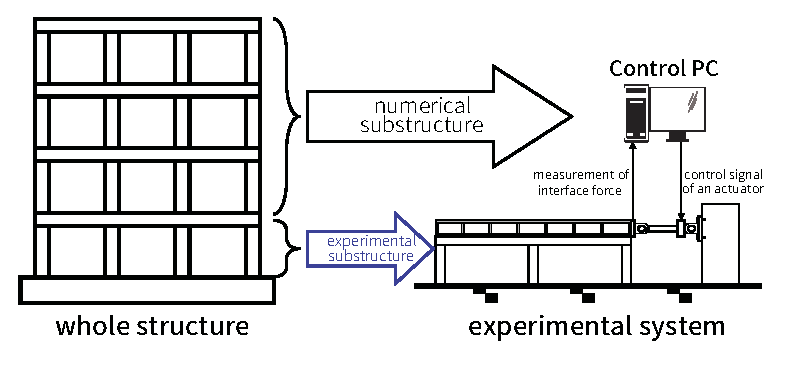
\includegraphics[scale =1] {figure/2_1a.eps}
   \label{fig:2-1a}
 }

 \subfigure[proposed method]{
   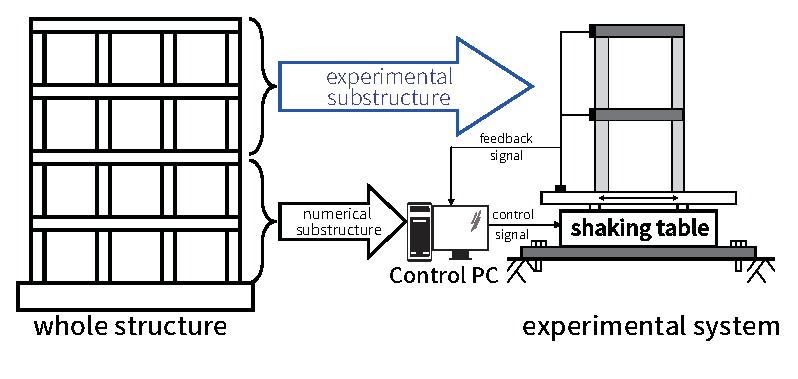
\includegraphics[scale =1] {figure/2_1b.eps}
   \label{fig:2-1b}
 }

\label{fig:2-1}
\caption{Conceptual illustrations of the substructuring methods}
\end{figure}

On these backgrounds, this subsection proposes a shaking table testing method using the upper part of a building structure as the experimental substructure based on the acceleration feedback from the experimental substructure. Also, the proposed method is verified experimentally through real-time implementation. Figure~\ref{fig:2-2} illustrates the schematic diagram of the proposed testing method in this study. At first, the interface force acting between the upper experimental and lower numerical substructures is calculated based on the acceleration feedback of the experimental substructure which is mounted on shaking table. Then the interface acceleration required to replicate the dynamic behavior of the whole structure is calculated from the numerical substructure subjected to the interface force and assumed base motion for the entire structure. Finally, shaking table excites the upper experimental substructure according to the command signal from the shaking table controller. The series of above processes are performed during a single time interval and repeated over the entire duration of the experiment.

\begin{figure}[ht]
\centering
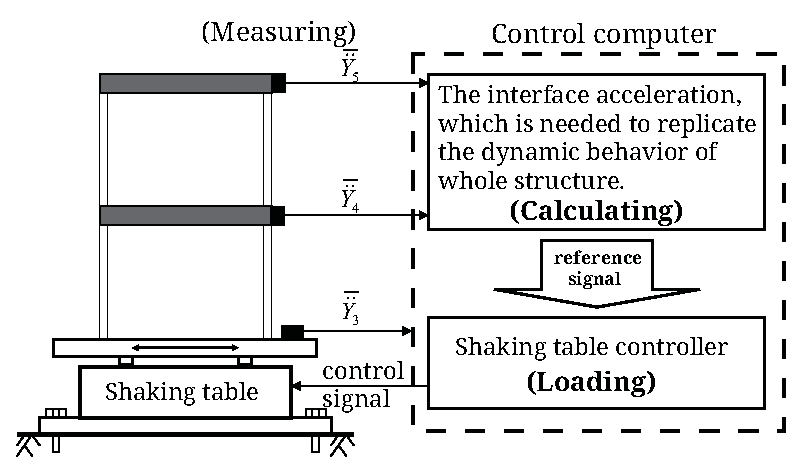
\includegraphics[scale =1] {figure/2-2.eps}
\label{fig:2-2}
\caption{Schematic diagram of the proposed method}
\end{figure}

\subsection{Formulation and Implementation Methodology}
\subsubsection{Experimental and Numerical Substructures}\label{2-2-1}
This subsection addresses physical interpretation and formulation of splitting the whole structure into the experimental and numerical substructures. A two-step process is carried out to formulate the equations of motion for those two substructures; separating the experimental substructure from the whole structure and constructing experimental substructure mounted on the shaking table and numerical substructures with external loads on the cutting plane, as shown in Figure~\ref{fig:2-3}. 

The equation of motion of the whole shear-type building structure subjected to the ground acceleration, $\ddot{Y}_g (t)$, is represented in Figure~\ref{fig:2-3a} and expressed as

\begin{equation}\label{eq:2-1}
\matr{M}\matr{\ddot{Y}}(t)+\matr{C}\matr{\dot{Y}}(t)+\matr{K}\matr{Y}(t) = \matr{p}(t)
\end{equation}

where, $\matr{Y}(t)$ is the $n \times 1$ vector of the absolute floor displacements given by $\left\{Y_{1},Y_{2},...,Y_{n}\right\}^{\top}$, and $\matr{p}(t)$ is the $n \times 1$ vector of the external force given by $\left\{0,...,0,c_{1}\dot{Y}_{g}(t)+k_{1}Y_{g}(t)\right\}^{\top}$, $\matr{M}$, $\matr{C}$ and $\matr{K}$ are the structural mass, damping and stiffness matrices, respectively, and expressed as follows.

\begin{equation}\label{eq:2-2}
\begin{aligned}
\matr{M} = \begin{bsmallmatrix} m_{n}&&&&&&\\&m_{n-1}&&&&&\\&&\ddots&&&&\\ \hline&&&m_{m}&&&\\&&&&m_{m-1}&&\\&&&&&\ddots&\\&&&&&&m_{1} \end{bsmallmatrix},\\
\matr{C} = \begin{bsmallmatrix} c_{n}&-c_{n}&&&&&\\-c_{n}&c_{n}+c_{n-1}&-c_{n-1}&&&&\\&\ddots&\ddots&\ddots&&&\\\hline&&-c_{m+1}&c_{m+1}+c_{m}&-c_{m}&&\\&&&-c_{m}&c_{m}+c_{m-1}&-c_{m-1}&\\&&&&\ddots&\ddots&\ddots&\\&&&&&-c_{2}&c_{2}+c_{1} \end{bsmallmatrix},\\
\matr{K} = \begin{bsmallmatrix} k_{n}&-k_{n}&&&&&\\-k_{n}&k_{n}+k_{n-1}&-k_{n-1}&&&&\\&\ddots&\ddots&\ddots&&&\\\hline&&-k_{m+1}&k_{m+1}+k_{m}&-k_{m}&&\\&&&-k_{m}&k_{m}+k_{m-1}&-k_{m-1}&\\&&&&\ddots&\ddots&\ddots&\\&&&&&-k_{2}&k_{2}+k_{1} \end{bsmallmatrix}
\end{aligned}
\end{equation}

The experimental and numerical substructures are separated from the whole structure by cutting at their interface, as shown in Figure~\ref{fig:2-3b}. Mathematically, this operation means separating the equations included in Eq.~\eqref{eq:2-1} into two groups of which one corresponds to the upper part DOF, and the other corresponds to the lower part DOF. The dotted line in Eq.~\eqref{eq:2-2} divides those two groups, and the resulting two equations of motions are written as

\begin{equation}\label{eq:2-3}
\matr{M}_{E}\matr{\ddot{Y}}_{E}(t)+\matr{C}_{E}(t)\matr{\dot{Y}}_{E}(t)+\matr{K}_{E}\matr{Y}_{E}(t) = \matr{p}_{E}(t)
\end{equation}

\begin{equation}\label{eq:2-4}
\matr{M}_{N}\matr{\ddot{Y}}_{N}(t)+\matr{C}_{N}(t)\matr{\dot{Y}}_{N}(t)+\matr{K}_{N}\matr{Y}_{N}(t) = \matr{p}_{N}(t)
\end{equation}

where, subscripts $E$ and $N$ denote the experimental and numerical substructures, respectively. $\matr{Y}_{E}$ and $\matr{Y}_{N}$ are an $l \times 1$ vector given by $\left\{Y_{E(1)},Y_{E(2)},\right.$ $\left....,Y_{E(l)}\right\}^{\top}$ and an $m \times 1$ vector given by $\left\{Y_{N(1)},Y_{N(2)},...,Y_{N(m)}\right\}^{\top}$, respectively. Accordingly, $n$, the length of the displacement vector, shown in Eq.~\eqref{eq:2-1} equals to $m+l$. Also, $Y_{E(1)}$, $Y_{E(l)}$, $Y_{N(1)}$ and $Y_{N(m)}$ in Eq.'s \eqref{eq:2-3} and \eqref{eq:2-4} correspond to $Y_{m+1}$, $Y_{n}$, $Y_{1}$ and $Y_{m}$ in Eq.~\eqref{eq:2-1}, respectively. The mass, damping and stiffness matrices and the external force vectors in Eq.~\eqref{eq:2-3} and \eqref{eq:2-4} are expressed as follows.

\begin{equation}\label{eq:2-5}
\begin{aligned}
\matr{M}_{E} = \begin{bsmallmatrix} m_{E(l)}&&&&\\&m_{E(l-1)}&&&\\&&\ddots&&\\&&&m_{E(2)}&\\&&&&m_{E(1)} \end{bsmallmatrix},\\
\matr{C}_{E} = \begin{bsmallmatrix} c_{E(l)}&-c_{E(l)}&&&&\\-c_{E(l)}&c_{E(l)}+c_{E(l-1)}&-c_{E(l-1)}&&\\&\ddots&\ddots&\ddots&\\&&-c_{E(3)}&c_{E(3)}+c_{E(2)}&-c_{E(2)}\\&&&-c_{E(2)}&c_{E(2)}+c_{E(1)} \end{bsmallmatrix},\\
\matr{K}_{E} = \begin{bsmallmatrix} k_{E(l)}&-k_{E(l)}&&&&\\-k_{E(l)}&k_{E(l)}+k_{E(l-1)}&-k_{E(l-1)}&&\\&\ddots&\ddots&\ddots&\\&&-k_{E(3)}&k_{E(3)}+k_{E(2)}&-k_{E(2)}\\&&&-k_{E(2)}&k_{E(2)}+k_{E(1)} \end{bsmallmatrix}
\end{aligned}
\end{equation}

\begin{equation}\label{eq:2-6}
\begin{aligned}
\matr{M}_{N} = \begin{bsmallmatrix} m_{N(m)}&&&&\\&m_{N(m-1)}&&&\\&&\ddots&&\\&&&m_{N(2)}&\\&&&&m_{N(1)} \end{bsmallmatrix},\\
\matr{C}_{N} = \begin{bsmallmatrix} c_{N(m)}&-c_{N(m)}&&&&\\-c_{N(m)}&c_{N(m)}+c_{N(m-1)}&-c_{N(m-1)}&&\\&\ddots&\ddots&\ddots&\\&&-c_{N(3)}&c_{N(3)}+c_{N(2)}&-c_{N(2)}\\&&&-c_{N(2)}&c_{N(2)}+c_{N(1)} \end{bsmallmatrix},\\
\matr{K}_{N} = \begin{bsmallmatrix} k_{N(m)}&-k_{N(m)}&&&&\\-k_{N(m)}&k_{N(m)}+k_{N(m-1)}&-k_{N(m-1)}&&\\&\ddots&\ddots&\ddots&\\&&-k_{N(3)}&k_{N(3)}+k_{N(2)}&-k_{N(2)}\\&&&-k_{N(2)}&k_{N(2)}+k_{N(1)} \end{bsmallmatrix}
\end{aligned}
\end{equation}

\begin{equation}\label{eq:2-7}
\matr{p}_{E}(t) = \left\{0,...,0,c_{E(1)}\dot{Y}_{N(m)}+k_{E(1)}Y_{N(m)}\right\}^{\top}
\end{equation}

\begin{equation}\label{eq:2-8}
\begin{aligned}
\matr{p}_{N}(t) ={}& \left\{c_{E(1)}\left(\dot{Y}_{E(1)}-\dot{Y}_{N(m)}\right)+k_{E(1)}\left(Y_{E(1)}-Y_{N(m)}\right),0,...\right. \\{}& \left. ,0,c_{1}\dot{Y}_{g}(t)+k_{1}Y_{g}(t)\right\}^{\top}
\end{aligned}
\end{equation}

\begin{figure}[ht]
\centering
\subfigure[Whole structure]{
   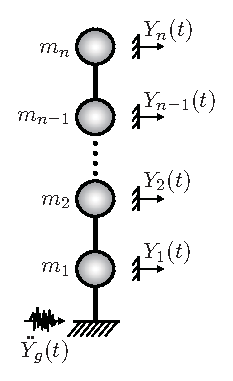
\includegraphics[width=0.2\textwidth] {figure/2-3a.eps}
   \label{fig:2-3a}
 }\hfill
 \subfigure[Separation of whole structure]{
   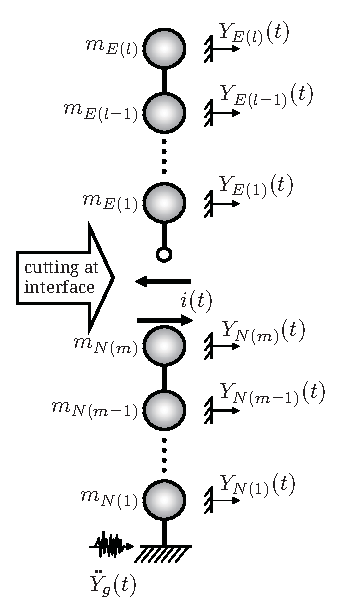
\includegraphics[width=0.3\textwidth] {figure/2-3b.eps}
   \label{fig:2-3b}
 }\hfill
 \subfigure[Experimental and numerical substructure]{
   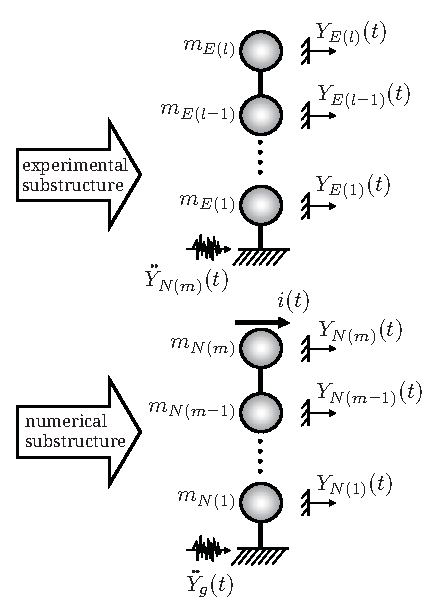
\includegraphics[width=0.4\textwidth] {figure/2-3c.eps}
   \label{fig:2-3c}
 }
\caption{Concept of the proposed method}
\label{fig:2-3}
\end{figure}

It is obvious from Eq.~\eqref{eq:2-7} that the absolute acceleration of the top story of the numerical substructure acts as the ground acceleration of the experimental substructure given by Eq.~\eqref{eq:2-3}. This condition is physically realized by synchronizing the shaking table motion with the absolute acceleration of the top story of the numerical substructure. Besides, the first element of the external force vector in Eq.~\eqref{eq:2-8} means the interface force acting on the top story of the numerical substructure. This interface force, which is denoted by $i(t)$ from now on, is produced by the damping and restoring forces of the first story in the upper experimental substructure and rewritten as follows.

\begin{equation}\label{eq:2-9}
i(t)=c_{E(1)}\left(\dot{Y}_{E(1)}-\dot{Y}_{N(m)}\right)+k_{E(1)}\left(Y_{E(1)}-Y_{N(m)}\right)
\end{equation}

As a result, the numerical substructure, of which equation of motion is given by Eq.~\eqref{eq:2-4}, is subjected to both the interface force at the top story and the ground motion at the base. The boundary condition and external load of each substructure are illustrated in Figure~\ref{fig:2-3c}.


\subsubsection{Measurement of the interface force}

In this section, the interface force, $i(t)$, which should be fed-back to the numerical substructure for calculating the interface acceleration, is indirectly measured by the accelerometers attached on the experimental substructure, as shown in Figure~\ref{fig:2-2}. Dynamic equilibrium in the experimental substructure is applied to derive the interface force using acceleration response measurement of the experimental substructure. As shown in Figure~\ref{fig4:dynamic}, dynamic equilibrium in the experimental substructure is established between the interface force acting at its base and the resultant of its inertial forces, because internal forces between each story are canceled with each other. This relation can be derived in another way. First, the dotted parts are shown in Eq.~\eqref{eq:2-5} are moved to the right side of Eq.~\eqref{eq:2-3}. Then the relation of Eq.~\eqref{eq:2-9} is applied to the right side. Finally, the summation of $l$ simultaneous equations for each side gives following expression of the interface force, $i(t)$.

\begin{equation}\label{eq:2-10}
i(t)=-\sum_{i=1}^{l}m_{E(i)}\ddot{Y}_{E(i)}
\end{equation}

Eq.~\eqref{eq:2-10} physically implies that the interface force, which is required as an input data of the numerical substructure, can be calculated using the measured acceleration responses of the experimental substructure.

\begin{figure}[ht]
\centering
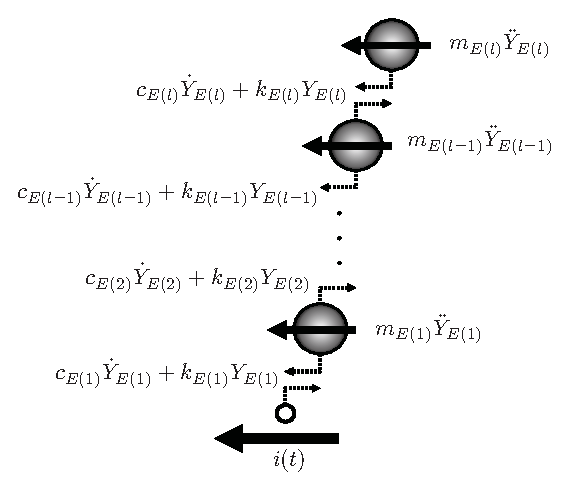
\includegraphics[width=0.6\textwidth] {figure/2-4.eps}
\caption{Dynamic equilibrium in experimental substructure}
\label{fig4:dynamic}
\end{figure}

\subsubsection{Calculation of the numerical substructure}
The calculation of the numerical substructure shown in Figure~\ref{fig:2-2} means on-line time history analysis of the Eq.~\eqref{eq:2-4} that represents the dynamic equilibrium of the numerical substructure shown in Figure~\ref{fig:2-3c}. To integrate this analysis procedure with shaking table control process implemented on a digital computer, Eq.~\eqref{eq:2-4} is transformed into state-space equations. The state-space equations, of which the output is the absolute accelerations of the numerical substructure, are given by the following equations in the continuous time domain.

\begin{equation}\label{eq:2-11}
\begin{aligned}
\matr{\dot{z}}(t)=\matr{A}\matr{z}(t)+\matr{B}\matr{u}(t)\\
\matr{O}(t)=\matr{C}\matr{z}(t)+\matr{D}\matr{u}(t)
\end{aligned}
\end{equation}

where, $\matr{z}(t)$ is the $2m \times 1$ vector of state variables composed of the relative displacement and velocity of the numerical substructure. $\matr{u}(t)$ is the $2 \times 1$ vector of input variables given by $\left\{i(t),\ddot{Y}_{g}(t)\right\}^{\top}$, in which the interface force, $i(t)$, is fed-back from the experimental substructure using Eq.~\eqref{eq:2-10}. $\matr{O}(t)$ is the $m \times 1$ vector of the output composed of the absolute accelerations of the numerical substructure.  The system matrices $\matr{A}$, $\matr{B}$, $\matr{C}$ and $\matr{D}$ have the dimension of $2m \times 2m$, $2m \times 2$, $m \times 2m$ and $m \times 2$, respectively, and are expressed as

\begin{align}
\matr{A}=&\begin{bmatrix} \matr{0}_{m\times m}&\matr{I}_{m\times m}\\-\matr{M}_{N}^{-1}\matr{K}_{N}&-\matr{M}_{N}^{-1}\matr{C}_{N} \end{bmatrix} \label{eq:2-12} \\
\matr{B}=&\begin{bmatrix} \matr{0} & \matr{0} \\ \matr{M}_{N}^{-1}\matr{b}&\matr{-1} \end{bmatrix} \label{eq:2-13} \\
\matr{C}=&\begin{bmatrix} -\matr{M}_{N}^{-1}\matr{K}_{N} & -\matr{M}_{N}^{-1}\matr{C}_{N} \end{bmatrix}\label{eq:2-14} \\
\matr{D}=&\begin{bmatrix} \matr{M}_{N}^{-1}\matr{b} & \matr{0} \end{bmatrix} \label{eq:2-15}
\end{align}

where, $\matr{0}$ and $\matr{I}$ are $m \times m$ zero and unit matrices, respectively, and $\matr{0}$ and $\matr{-1}$ are an $m \times 1$ vector of $0$ and an $m \times 1$ vector of $-1$, respectively. $\matr{b}$ is an $m \times 1$ vector given by $\left\{1, 0, ..., 0 \right\}^{\top}$. Eq.~\eqref{eq:2-11} with the inputs of the interface force and ground motion is incorporated in the `Calculating' part shown in Figure~\ref{fig:2-2}, and produces the absolute acceleration responses of the numerical substructure on-line. Among those acceleration responses, the one corresponding to the top story is utilized as the reference signal to operate shaking table.

\subsection{Numerical Substructure}
For the verification experiment of the proposed methodology, the object structure is assumed to be a five-story shear type building structure, of which two upper stories are assumed to be the experimental substructure as shown in Fifure~\ref{fig:2-8}. As a result, the numerical substructure is the three lower stories of the whole structure. For the construction of the finite element model of the numerical substructure, the inter-story damping and stiffness coefficients of the shear-type experimental substructure are identified based on the measured acceleration responses, and the mass of the two floors are measured directly. The system identification of the experimental substructure is conducted using the command \code{fmincon} in MATLAB\citep{coleman1999optimization}, which uses the interior-reflective Newton method to solve the constrained nonlinear minimization problem \citep{coleman1994convergence,coleman1996interior}. Resulting identified parameters can be summarized as follow.

\begin{equation}\label{eq:2-18}
\begin{aligned}
m_{E(1)}=m_{4}=2.04(kg),~& m_{E(2)}=m_{5}=5.10(kg)\\
k_{E(1)}=k_{4}=45.3(N/m),~& k_{E(2)}=k_{5}=48.5(N/m)\\
c_{E(1)}=c_{4}=0.023(N\cdot s/m),~&c_{E(2)}=c_{5}=0.015(N\cdot s/m)
\end{aligned}
\end{equation}

which correspond to the first and second natural frequencies of $2.5$ and $8.6Hz$, respectively, as given in Table~\ref{tab:2-1}. Figure~\ref{fig:2-10} compares the experimentally obtained transfer functions with numerically computed ones. As shown in Figure~\ref{fig:2-10}, measured transfer functions agree well with those of the corresponding numerical model.

\begin{figure}[ht]
\centering
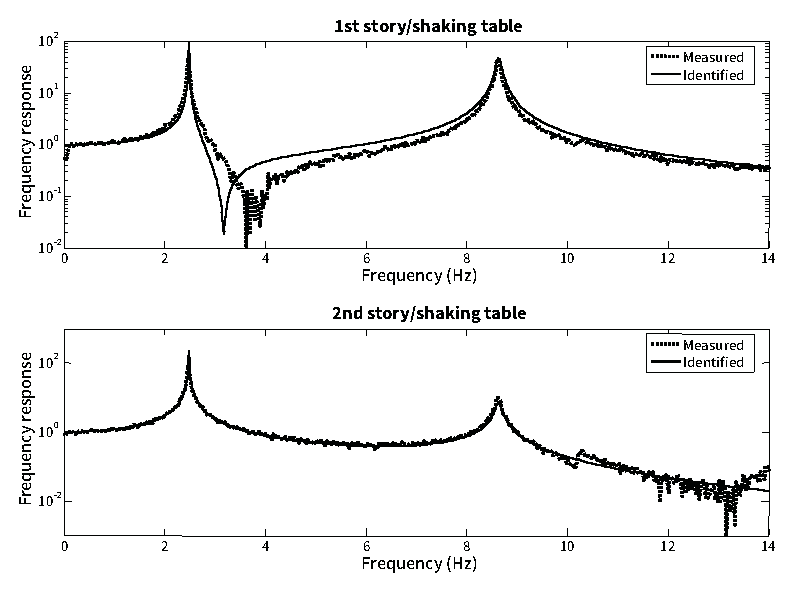
\includegraphics[width=0.8\textwidth] {figure/2-10.eps}
\caption{Comparison of experimental and approximated transfer functions.}
\label{fig:2-10}
\end{figure}

\begin{table}[ht]
\centering
\begin{tabularx}{\textwidth}{@{}X|X|X@{}}
\toprule[1pt]\midrule[0.3pt]
Mode&Frequency components(Hz) observed in the experimental substructure with 2 DOFs&Natural frequencies (Hz) of the whole structure with 5 DOFs\\ \hline
1&1.3&1.3\\
2&2.5&4.2\\
3&4.2&7.1\\
4&7.1&9.4\\
5&8.6&10.8\\ \bottomrule
\end{tabularx}
\caption{Frequencies observed in the time records of the experimental substructure from the test without feedback and the natural frequencies of the assumed whole structure}
\label{tab:2-1}
\end{table}

The structural parameters for the first story of the experimental structure given in Eq.~\eqref{eq:2-18} are applied to all stories of the numerical substructure and summarized as the following:

\begin{align}
i(t)=&-m_{E(1)}\ddot{Y}_{E(1)}(t)-m_{E(2)}\ddot{Y}_{E(2)}(t) \label{eq:2-19} \\
\ddot{Y}_{N(3)}(t)=&-c_{N(3)}\left(\dot{Y}_{N(3)}-\dot{Y}_{N(2)}\right) -k_{N(3)}\left(Y_{N(3)}-Y_{N(2)}\right)+i(t) \label{eq:2-20}
\end{align}

Eq.~\eqref{eq:2-20} means that the interface force, which is produced by the shaking table, is calculated using the two measured absolute accelerations of the experimental substructure. Then, the interface acceleration is calculated from the numerical substructure expressed by Eq.~\eqref{eq:2-11}. Figure~\ref{fig:2-11} represents the block diagram of the entire substructuring testing system including the numerical substructure marked by the shaded area. In Figure~\ref{fig:2-11}, the ground acceleration, $\ddot{Y}_{g}$, is not a measured signal but an input data prescribed by a user. Finally, the shaking table motion is controlled using the inverse transfer function of Eq.~\eqref{eq:2-17} to minimize the errors between the interface acceleration computed as the third story absolute acceleration of the numerical substructure, $\ddot{Y}_{N(3)}$, and the actual shaking table acceleration. Therefore, the shaking table itself works as the interface node of Figure~\ref{fig:2-3b} and excites the upper experimental substructure. In the actual implementation of the shaking table test, the continuous filters included in Figure~\ref{fig:2-11} are converted into discrete filters with a time step of 0.01 sec.

\begin{figure}[ht]
\centering
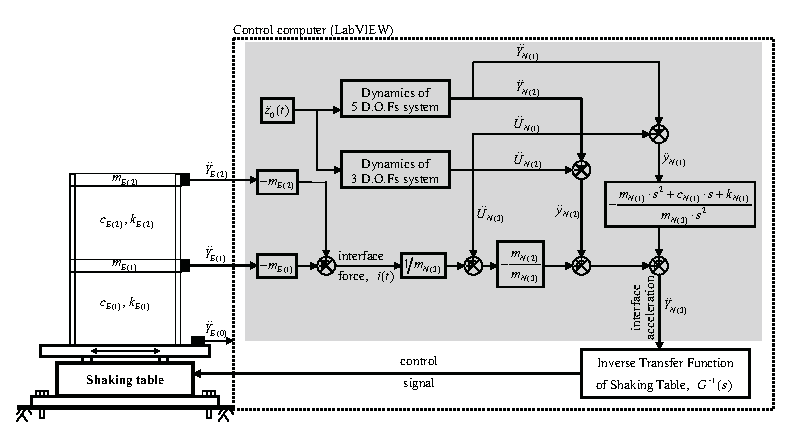
\includegraphics[width=0.8\textwidth] {figure/2-11.eps}
\caption{Block diagram of the integrated controller for the substructuring testing system.}
\label{fig:2-11}
\end{figure}







%!TEX encoding = UTF-8 Unicode
\section{Hybrid Testing Method for the Performance Evaluation of a Tuned Liquid Damper}% hybrid testing method for the Performance Evaluation of a Tuned Liquid Column Damper
\label{chap:3}

In this section, the vibration control effect of a TLD for a building structure excited by earthquake load is experimentally evaluated through the hybrid testing method. The hybrid testing method does not require a physical building structural model in performing the experiment of a TLD–structure interaction system, and it only uses a TLD which is known to have strong nonlinearity dependent on response amplitude, excitation frequency, and depth to length ratio\citep{yu1999non}. The structural responses of the interaction system are calculated numerically in real time using the analytical structural model with the excitations of measured control force, user-defined base earthquake loads, and its state space realization incorporated in the integrated controller of the shaking table. Also, in order to minimize the distortion of the acceleration of the shaking table, the inverse transfer function of the shaking table is identified, and its state space realization is implemented in the shaking table controller. The motion of shaking table behaves both the controlled and uncontrolled absolute acceleration of the TLD mounted floor by modulating the feedback gain of the shear force measured by the load cell installed between the TLD and the shaking table. Comparison between the structural responses obtained by the hybrid testing method and the conventional shaking table test of a single story steel frame with TLD is made in order to verify the accuracy of the hybrid testing method and the uncontrolled and TLD-controlled structural responses of a three-story structure are obtained by the hybrid testing method in both time and frequency domains.

\subsection{Hybrid Testing Method with TLD}
Figure~\ref{fig:3-1} depicts the conceptual illustrations of the hybrid testing method for an n-degrees-of-freedom structural model which is excited by base acceleration and has a tuned liquid damper at its top story. First, the whole control system is separated into the lower part structure, and the upper part TLD and the interaction force between the structure and TLD are considered. The TLD with the interacting force at its bottom is physically tested, and the response of the structure with interacting force at the top floor and the base acceleration is numerically calculated by using the computer controlling the motion of the shaking table. Measurement of interacting force is easily accomplished by installing a shear-type load-cell at the bottom of the TLD, as shown in Figure~\ref{fig:3-1}. TLD-generated shear force is fed back to the control computer. With this fed-back interacting force, the structural response of the story, where a TLD is installed, is calculated using the numerical part. The shaking table excites the upper TLD according to this calculated response. This process is carried out on real-time.

\begin{figure}[ht]
\centering
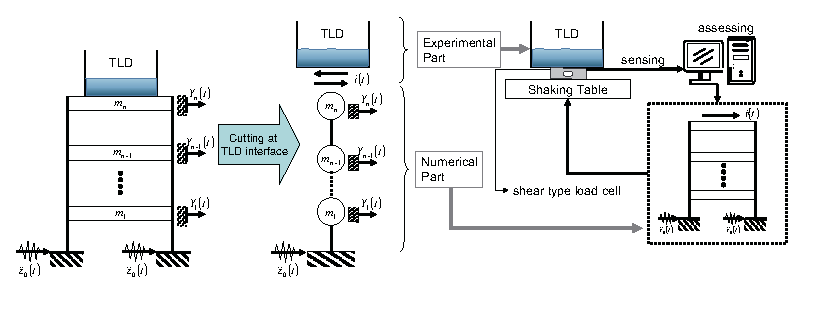
\includegraphics[width=\textwidth] {figure/3-1.eps}
\caption{Conceptual view of the hybrid shaking table test}
\label{fig:3-1}
\end{figure}

The numerical part with $n-$DOFs, which is subjected to the excitations of the measured control force, $i_{e}(t)$, and the input acceleration, $\ddot{z}_{0}(t)$, at its top and bottom, respectively, as enclosed in dotted line in Figure~\ref{fig:3-1}, is calculated by

\begin{equation}\label{eq:3-1}
\matr{M}\matr{\ddot{Y}}_{i}(t) + \matr{C}\matr{\dot{Y}}_{i}(t) + \matr{K}\matr{Y}_{i}(t) = \matr{p}(t)
\end{equation}

where, $\matr{Y}_{i}(t)$ is the absolute displacement at the $i$th$\left(i=1\rightarrow n\right)$ story, and the location vector of external forces with the length of $n$, $\matr{p}(t)$  equals to $\left\{ -i_{e}(t),0,...,0,c_{1}\dot{z}_{0}(t)+k_{1}z_{0}(t)\right\}^{\top}$, in which subscript ``$e$'' denotes the ``\textit{experimentally}'' measured interacting force. Also, the structural mass, damping and stiffness matrices are represented by

\begin{equation}\label{eq:3-2}
\begin{aligned}
\matr{M}=\begin{bsmallmatrix}m_{n}&&&\\&m_{n-1}&&\\&&\ddots&m_{1}\end{bsmallmatrix},
\matr{C}=\begin{bsmallmatrix}c_{n}&-c_{n}&&\\-c_{n}&c_{n}+c_{n-1}&-c_{n-1}&\\ &\ddots&\ddots&\ddots\\&&-c_{2}&c_{2}+c_{1}\end{bsmallmatrix},\\
\matr{K}=\begin{bsmallmatrix}k_{n}&-k_{n}&&\\-k_{n}&k_{n}+k_{n-1}&-k_{n-1}&\\ &\ddots&\ddots&\ddots\\&&-k_{2}&k_{2}+k_{1}\end{bsmallmatrix}
\end{aligned}
\end{equation}

To calculate the numerical part such as Eq.~\eqref{eq:3-2} by a control computer on real-time, it is transformed into the state-space representation given by

\begin{equation}\label{eq:3-3}
\begin{aligned}
\matr{\dot{z}}(t)&=\matr{A}_{c}\matr{z}(t)+\matr{B}_{c}\matr{u}(t)\\
\matr{O}(t)&=\matr{C}_{c}\matr{z}(t)+\matr{D}_{c}\matr{u}(t)
\end{aligned}
\end{equation}

where, the state variable vector, $\matr{z}(t)$, with the length of $2n$ comprises the state variables, $\left\{\matr{y}_{i}(t),\matr{\dot{y}}_{i}(t)\right\}^{\top}$, in which the structural relative displacement, $\matr{y}_{i}(t)$, equals to $\matr{Y}_{i}(t)-z_{0}(t)$. The input vector, $\matr{u}(t)$, with the length of 2 consists of $\left\{-i_{e}(t), \ddot{z}_{0}\right\}^{\top}$. The output vector, $\matr{O}(t)$, with the length of $n$ corresponds to the structural absolute acceleration, $\matr{\ddot{Y}}_{i}(t)$, itself. The matrices $\matr{A}_{c}$, $\matr{B}_{c}$, $\matr{C}_{c}$ and $\matr{D}_{c}$ with the sizes of $2n \times 2n$, $2n \times 2$, $n \times 2n$ and $n \times 2$, respectively, are expressed as the following Eqs.~\eqref{eq:3-4}-\eqref{eq:3-7}.

\begin{align}
\matr{A}_{c}&=\begin{bmatrix} \matr{0}_{m\times n}&\matr{I}_{m \times n}\\-\matr{M}^{-1}\matr{K}&-\matr{M}^{-1}\matr{C}\end{bmatrix} \label{eq:3-4}\\
\matr{B}_{c}&=\begin{bmatrix} \matr{0}_{n\times 1}&\matr{0}_{n\times 1}\\ \matr{M}^{-1}\matr{b}&\matr{-1}\end{bmatrix} \label{eq:3-5}\\
\matr{C}_{c}&=\begin{bmatrix} -\matr{M}^{-1}\matr{K}&-\matr{M}^{-1}\matr{C}\end{bmatrix} \label{eq:3-6}\\
\matr{D}_{c}&=\begin{bmatrix} \matr{M}^{-1}\matr{b}&\matr{0}_{m \times 1}\end{bmatrix} \label{eq:3-7}
\end{align}


%!TEX encoding = UTF-8 Unicode
\section{Hybrid testing method for the Performance Evaluation of a Tuned Liquid Column Damper}
\label{chap:4}

The tuned liquid column damper has received the attention of researchers as a type of auxiliary mass system\citep{samali1998wind}. TLCD has the control characteristics similar to that of tuned mass damper, which is one of most frequently used dampers for vibration control. Since the viscosity term in the governing equation of motion of TLCD is a function of the absolute value of liquid velocity, the equation is nonlinear, and the dynamic characteristics of TLCD depend on the magnitude and the characteristics of excitation forces and the corresponding structural responses of the floor at which TLCD is installed\citep{yalla2001liquid}.
In this section, the vibration control effect of a TLCD for a building structure excited by earthquake load is experimentally evaluated through the hybrid testing method. The hybrid testing method does not require a physical building structural model in performing the experiment of a TLCD-structure interaction system, and it only uses a TLCD. The structural responses of the interaction system are calculated numerically in real time using the analytical structural model with the excitations of measured control force, user-defined base earthquake loads, and its state space realization incorporated in the integrated controller of the shaking table. Also, in order to minimize the distortion of the acceleration of the shaking table, the inverse transfer function of the shaking table is identified, and its state space realization is implemented in the shaking table controller. The shaking table behaves as the absolute acceleration of the TLCD mounted floor by calculating the fed back signal of the shear force signal measured by the load cell positioned between the TLCD and plate of the shaking table. Comparison results between the structural responses obtained by the hybrid testing method and the conventional shaking table test of a single story steel frame with TLCD are made to verify the accuracy of the hybrid testing method in both time and frequency domains.

\subsection{RHybrid Testing Method with TLCD}
Figure~\ref{fig:4-1} shows the conceptual view of the experiment. The whole structural control system, which a TLCD was installed onto the structural model with n-degrees-of-freedom at its top story, is separated, and as the result of that, the force interacts at their interface. The upper part of TLCD with the interacting force at its bottom is physically tested and the lower part of the structural model with the interacting force and the input motion at its top story and base, respectively, is numerically calculated within the computer to control the motion of shaking table. For the experimental implementation, interacting or control force generated by a TLCD, which is observed from a load-cell, is fed back to the control computer. With the fed-back interacting force, the structural response of the story, where a TLCD is incorporated, is calculated from the numerical part. The shaking table excites the upper TLCD with this calculated response. These processes are carried out on real-time.

\begin{figure}[ht]
\centering
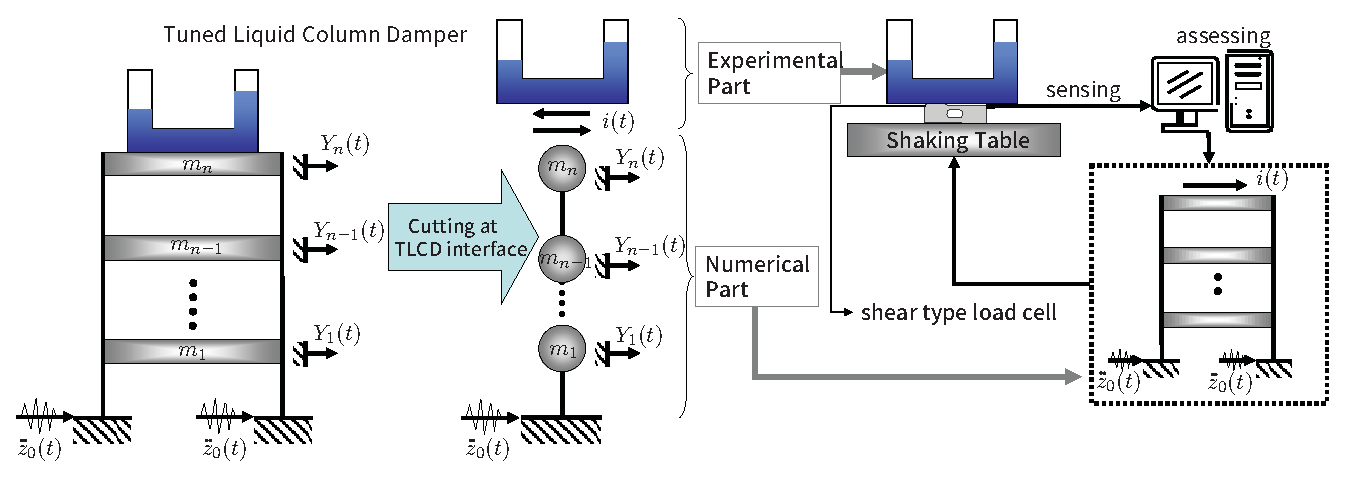
\includegraphics[width=1\textwidth] {figure/4-1.eps}
\caption{Concept of the hybrid testing method (TLCD)}
\label{fig:4-1}
\end{figure}

Of theses procedures, the numerical part with $n$-DOFs, which is subjected to the excitations of the experimentally measured control force, $i_{e}(t)$, and the input acceleration, $\ddot{z}_{0}(t)$, at its top and bottom, respectively, as enclosed in dotted line in Figure~\ref{fig:4-1}, is calculated by

\begin{equation}\label{eq:4-1}
\matr{M}\matr{\ddot{Y}}_{i}(t)+\matr{C}\matr{\dot{Y}}_{i}(t)+\matr{K}\matr{Y}_{i}(t)=\matr{p}(t)
\end{equation}

where, $\matr{Y}_{i}(t)$ is the absolute displacement at the $i$th$\left(i=1\rightarrow n\right)$ story, and the location vector of external forces with the length of $n$, $\matr{p}(t)$  equals to $\left\{ -i_{e}(t),0,...,0,c_{1}\dot{z}_{0}(t)+k_{1}z_{0}(t)\right\}^{\top}$, in which subscript ``$e$'' denotes the ``\textit{experimentally}'' measured interacting force. Also, the structural mass, damping and stiffness matrices are represented by

\begin{equation}\label{eq:4-2}
\begin{aligned}
\matr{M}=\begin{bsmallmatrix}m_{n}&&&\\&m_{n-1}&&\\&&\ddots&m_{1}\end{bsmallmatrix},
\matr{C}=\begin{bsmallmatrix}c_{n}&-c_{n}&&\\-c_{n}&c_{n}+c_{n-1}&-c_{n-1}&\\ &\ddots&\ddots&\ddots\\&&-c_{2}&c_{2}+c_{1}\end{bsmallmatrix},\\
\matr{K}=\begin{bsmallmatrix}k_{n}&-k_{n}&&\\-k_{n}&k_{n}+k_{n-1}&-k_{n-1}&\\ &\ddots&\ddots&\ddots\\&&-k_{2}&k_{2}+k_{1}\end{bsmallmatrix}
\end{aligned}
\end{equation}

To calculate the numerical part such as Eq.~\eqref{eq:3-2} by a control computer on real-time, it is transformed into the state-space representation given by

\begin{equation}\label{eq:4-3}
\begin{aligned}
\matr{\dot{z}}(t)&=\matr{A}_{c}\matr{z}(t)+\matr{B}_{c}\matr{u}(t)\\
\matr{O}(t)&=\matr{C}_{c}\matr{z}(t)+\matr{D}_{c}\matr{u}(t)
\end{aligned}
\end{equation}

where, the state variable vector, $\matr{z}(t)$, with the length of $2n$ comprises the state variables, $\left\{\matr{y}_{i}(t),\matr{\dot{y}}_{i}(t)\right\}^{\top}$, in which the structural relative displacement, $\matr{y}_{i}(t)$, equals to $\matr{Y}_{i}(t)-z_{0}(t)$. The input vector, $\matr{u}(t)$, with the length of 2 consists of $\left\{-i_{e}(t), \ddot{z}_{0}\right\}^{\top}$. The output vector, $\matr{O}(t)$, with the length of $n$ corresponds to the structural absolute acceleration, $\matr{\ddot{Y}}_{i}(t)$, itself. The matrices $\matr{A}_{c}$, $\matr{B}_{c}$, $\matr{C}_{c}$ and $\matr{D}_{c}$ with the sizes of $2n \times 2n$, $2n \times 2$, $n \times 2n$ and $n \times 2$, respectively, are expressed as the following Eqs.~\eqref{eq:4-4}-\eqref{eq:4-7}.

\begin{align}
\matr{A}_{c}&=\begin{bmatrix} \matr{0}_{m\times n}&\matr{I}_{m \times n}\\-\matr{M}^{-1}\matr{K}&-\matr{M}^{-1}\matr{C}\end{bmatrix} \label{eq:4-4}\\
\matr{B}_{c}&=\begin{bmatrix} \matr{0}_{n\times 1}&\matr{0}_{n\times 1}\\ \matr{M}^{-1}\matr{b}&\matr{-1}\end{bmatrix} \label{eq:4-5}\\
\matr{C}_{c}&=\begin{bmatrix} -\matr{M}^{-1}\matr{K}&-\matr{M}^{-1}\matr{C}\end{bmatrix} \label{eq:4-6}\\
\matr{D}_{c}&=\begin{bmatrix} \matr{M}^{-1}\matr{b}&\matr{0}_{m \times 1}\end{bmatrix} \label{eq:4-7}
\end{align}

where, $\matr{0}_{n \times n}$ and $\matr{I}_{n \times n}$ are the zero and unit matrices, respectively, with the size of $n\times n$. $\matr{0}_{n\times 1}$ and $\matr{-1}$ are the vector whose components are $0$ and $-1$, respectively, with the length of $n \times 1$. $\matr{b}$ equal to $\left\{1,0,...,0\right\}^{\top}$ with the length of $n \times 1$.


%!TEX encoding = UTF-8 Unicode
\section{Hybrid Testing Method for the Performance Evaluation of a Tuned Liquid Mass Damper}
\label{chap:5}

In previous study\citep{heo2009performance}, a new control device, which is called tuned liquid mass damper (TLMD), was developed and discussed in this section. The dynamic characteristics of a TLMD used in this study are that its mass is composed of both a mass of TLCD frame itself and that of liquid in a tank. Natural rubber columns were used to substitute the stiffness of a TMD. Therefore, a TLMD operates as a TLCD in one direction and behaves as a TMD in the other orthogonal direction. 

In this section, the control performance of the proposed TLMD for reducing bidirectional responses of building structures is experimentally verified through both a conventional structural testing method and hybrid testing method. First, the control performance of a TLMD is evaluated by forced vibrating sinusoidal signal to an experimental prototype which is composed of both a TLMD and a  building structure. Then, the hybrid testing method is performed to evaluate the performance of a TLMD, in which the building structural model is used as a numerical part, and the TLMD is experimentally tested.

\subsection{Developed TLMD Model}
Figure~\ref{fig:5-1} shows the plan view of the TLMD used in this study. The bidirectional TLMD would be installed in the POSCO New Songdo City Tower 1A in Incheon, South Korea with 64 stories and 236 meters in height. An eigenvalue analysis of the tower resulted in $0.182$ and $0.162Hz$ in the $x, y$-directions, respectively, for the first natural frequencies, and $34,000tons$ for the first modal mass. The total mass of the bidirectional TLMD is $600tons$ that results from the effective mass ratio of about $1.76\%$.

The experimental building and TLMD models were manufactured by applying the scaling factors given in Table~\ref{tab:5-1} to the first modal properties of the prototype tower. The building model with the parameters shown in Table~\ref{tab:5-2} was made by applying the scaling factors in Table\ref{tab:5-1} to the prototype building. Applying the scale $1/\sqrt{20}$ in frequency to the natural frequencies of a prototype model, $0.182$ and $0.162Hz$, gives $0.82$ and $0.73Hz$ in the $x-$ and $y-$directions, respectively. Also, the mass of a building structure is reduced by $4,250kg$. The stiffness of a building model is calculated to be $4250(kg)\times \left(2\pi \times 0.82(Hz)\right)^{2}\cong 110 000(N/m)$ in the $x-$direction and $4250(kg)\times \left(2\pi \times 0.73(Hz)\right)^{2} \cong 89,000(N/m)$ in the $y-$direction, respectively.

\begin{figure}[ht]
\centering
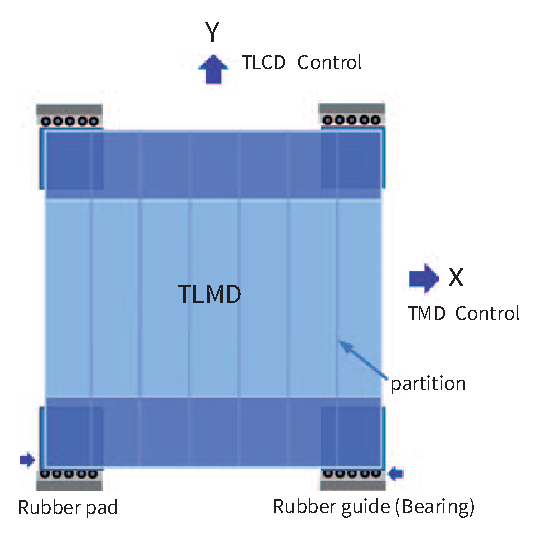
\includegraphics[width=0.8\textwidth] {figure/5-1.eps}
\caption{Concept of a TLMD}
\label{fig:5-1}
\end{figure}

\begin{table}[ht]
\centering
\begin{tabularx}{\textwidth}{@{}X|X|X@{}}
\toprule[1pt]\midrule[0.3pt]
Quantity & Dimension & Scaling factor\\ \hline
Length & $L$ & $1:20$\\
Mass & $M$ & $1:20^{3} = 1:8000$\\
Frequency (Hz) & $T^{-1}$ & $1:1/\sqrt{20} = 1:0.223$\\
Acceleration & $LT^{-2}$ & $1:1$\\
\bottomrule
\end{tabularx}
\caption{Similitude law applied to TLMD model}
\label{tab:5-1}
\end{table}

\begin{table}[ht]
\centering
\begin{tabularx}{\textwidth}{@{}X|X|X@{}}
\toprule[1pt]\midrule[0.3pt]
Design parameter & $y-$direction & $x-$direction\\ \hline
Siffness (N/m) & $88,000$ & $110,000$\\
Frequency (Hz) & $0.73$ & $0.82$\\
Mass (kg) & $4,250$ & $4,250$\\
\bottomrule
\end{tabularx}
\caption{Design parameters of the building model}
\label{tab:5-2}
\end{table}

\begin{table}[ht]
\centering
\begin{tabularx}{\textwidth}{@{}X|X|X@{}}
\toprule[1pt]\midrule[0.3pt]
Design parameters & TLCD control direction & TMD control direction\\ \hline
Siffness or liquid length & $0.98m$ (liquid length) & $1990N/m$ (stiffness)\\
Frequency (Hz) & $0.73$ & $0.82$\\
Mass (kg) & $35$ & $75$\\
\bottomrule
\end{tabularx}
\caption{Design parameters of a TLMD model}
\label{tab:5-3}
\end{table}

As shown in Table~\ref{tab:5-3}, it is obvious that the natural frequencies of a TLMD tune to those of a building structure in the TMD$(x)$ and TLCD$(y)$-control directions, respectively. The masses of a TLMD with the ratios of $1.8$ and $0.8\%$ to the mass of a building model become $75kg$ in the TMD-control and $32kg$ in the TLCD-control directions, respectively. The stiffness of rubber columns used in a TMD, $k$, and the liquid length of a TLCD, $L$, are determined by

\begin{align}
k&=m\left(2\pi f_{m}\right)^{2} \label{eq:5-1} \\
L&=\frac{2g}{\left(2\pi f_{L}\right)^{2}} \label{eq:5-2}
\end{align}

where $m$ and $f_{m}$ are the mass and the tuned frequency of a TLCD, respectively, in the TMD-control direction. $g$ and $f_{L}$ are the gravity acceleration and the tuned frequency of the TLCD, respectively, in the TLCD-control direction. With these relations, the final parameters of a TLMD are shown in Table~\ref{tab:5-3}.








\clearpage
\section{Design of Experimental Controller}
\subsection{Experimental System for Substructurubg Technique}

The experimental system is shown in Figure~\ref{fig:2-5} and \ref{fig:2-6} was equipped in Seismic Retrofitting \& Remodeling Research Center at the Dankook University, Seoul, Korea. The test structure (the experimental substructure) used in this experiment is a two-story steel frame with a single bay. The height and width of the experimental substructure are 1.0 and 0.6 m, respectively. The first floor mass, $m_{E(1)}$, and the second floor mass, $m_{E(2)}$, are 2.04 and 5.10 kg, respectively. The experimental substructure is excited by a uni-axial shaking table. The accelerometers are attached to each floor of the experimental substructure to measure its absolute floor acceleration responses. Additionally, an accelerometer is placed on the shaking table to monitor its motion. The data acquisition and implementation of the digital shaking table controller are performed using a real-time digital signal processor (DSP). The major task of the data acquisition board is to carry out the analog-to-digital (A/D) conversion of the measured acceleration data and the digital-to-analog (D/A) conversion of the reference signal computed by the shaking table controller, which is programmed using LabVIEW \citep{bishop2007labview}. An 8-channel data acquisition system was employed using an NI PCI-6052E board and an NI SC-2345 BNC cable connector as a signal conditioner.

\begin{figure}[ht]
\centering
\includegraphics[width=0.8\textwidth] {figure/2-5.eps}
\caption{Overall view of experimental system}
\label{fig:2-5}
\end{figure}

\begin{figure}[ht]
\centering
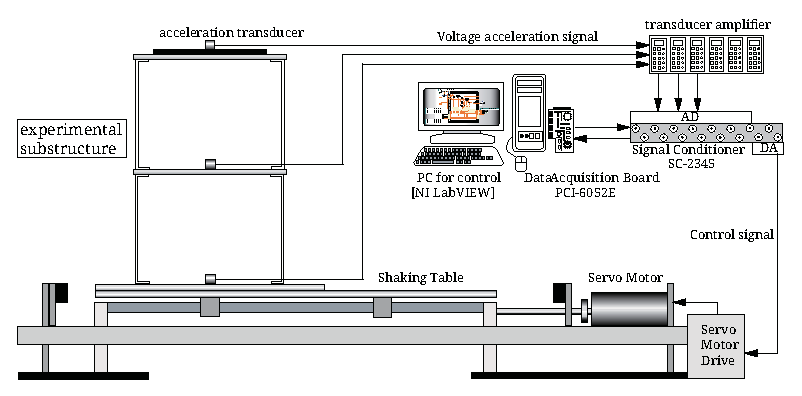
\includegraphics[width=0.8\textwidth] {figure/2-6.eps}
\caption{Schematic diagram of experimental system}
\label{fig:2-6}
\end{figure}

\subsection{Shaking table controller}
The composition of the experimental system is illustrated in Figure~\ref{fig:2-6}. The shaking table shown in Figure~\ref{fig:2-6} moves in accordance with the control signal, which is generated by the control computer and sent through D/A conversion board. In almost every case, the target acceleration signal and actual acceleration produced by the shaking table are different in their amplitudes and phases due to the shaking table dynamics. Therefore, in order to compensate the distortion of the actual shaking table acceleration against the shaking table dynamics existing between the reference signal and the actual measured acceleration of the shaking table, the inverse transfer function of the actual acceleration of shaking table with respect to the command signal generated by the control computer is constructed and implemented in the shaking table control computer as shown in Figure~\ref{fig:2-8}. First, the inverse transfer function, of which amplitude and phase are represented in Figure~\ref{fig:2-7} by the dashed line, is obtained experimentally. Then, the experimental inverse transfer function is approximated by a rational function for its implementation in the control computer. In this verification experiment, the inverse transfer function of the shaking table is approximated using the command \code{invfreqs} in MATLAB \citep{little1992signal}, which adopts the damped Gauss-Newton method for the iterative search to minimize the sum of the squared error between the measured and the desired frequency response points\citep{dennis1983numerical}. The approximation result is given by the following 5-th order linear filter and compared with the experimental one in Figure~\ref{fig:2-7}. 

\begin{figure}[ht]
\centering
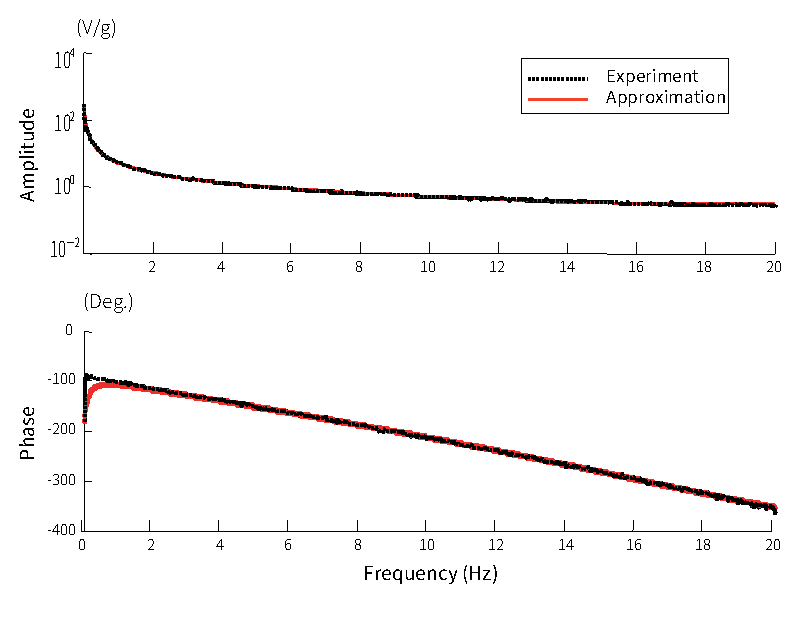
\includegraphics[width=0.8\textwidth] {figure/2-7.eps}
\caption{Inverse transfer function of shaking table}
\label{fig:2-7}
\end{figure}

Inverse transfer function, Eq.~\eqref{eq:2-16}, corresponds to the shaking table controller of Figure~\ref{fig:2-2}. 

\begin{equation}\label{eq:2-16}
G^{-1}(s) = \frac{0.6s^5 + 94s^4 + 10746s^3 + 498200s^2 + 167124s + 108216}{s^5 + 204s^4 + 15900s^2 + 8252s^2 + 4676s + 405}
\end{equation}

\begin{figure}[ht]
\centering
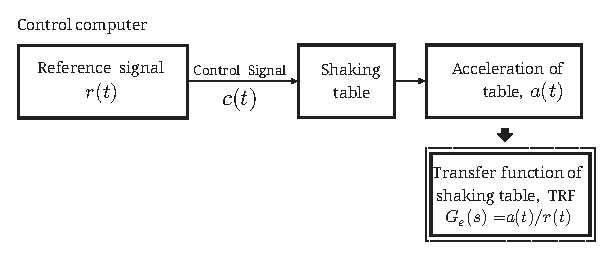
\includegraphics[width=0.8\textwidth] {figure/5-13.eps}
\caption{Definition of the transfer function of shaking table}
\label{fig:5-13}
\end{figure}

\begin{figure}[ht]
\centering
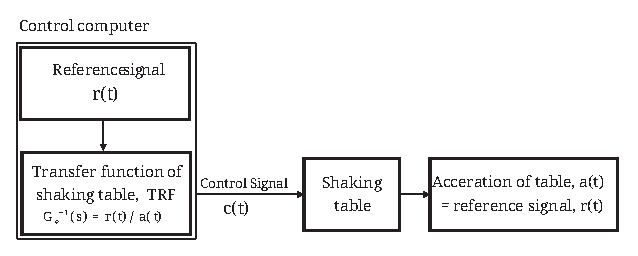
\includegraphics[width=0.8\textwidth] {figure/5-14.eps}
\caption{Compensation using the inverse transfer function of shaking table}
\label{fig:5-14}
\end{figure}

For the implementation in the digital computer, Eq.~\eqref{eq:2-16} is realized into the following state equation.

\begin{equation}\label{eq:2-17}
\begin{aligned}
\matr{\dot{x}}_{c} = \matr{A}_{c}\matr{x}_{c} + \matr{B}_{c}r_{c}\\
y_{c}=\matr{C}_{c}\matr{x}_{c}+D_{c}r_{c}
\end{aligned}
\end{equation}

where, $\matr{x}_{c}$, $r_{c}$ and $y_{c}$ is the state vector, the reference signal, the control signal of the shaking table controller, respectively. $\matr{A}_{c}$, $\matr{B}_{c}$, $\matr{C}_{c}$ and $D_{c}$ is the $5\times5$ state matrix, the $5\times1$ reference signal influence matrix, the $1\times5$ output matrix and the coupling coefficient between the reference and control signal.

\begin{figure}[ht]
\centering
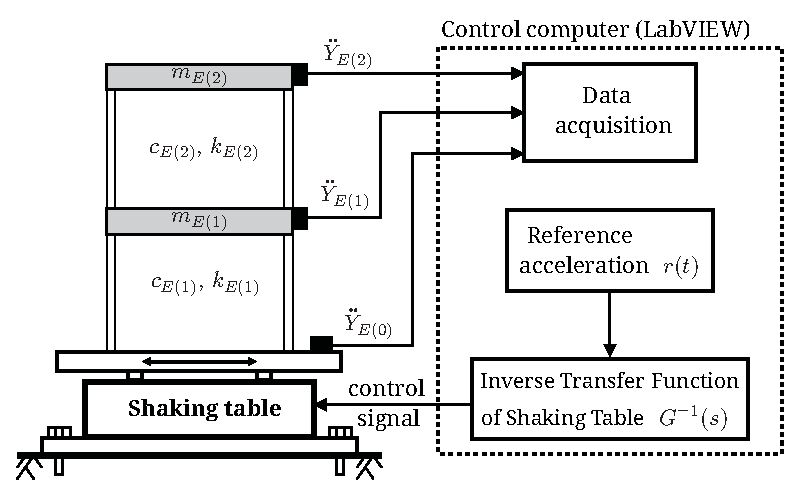
\includegraphics[width=0.8\textwidth] {figure/2-8.eps}
\caption{Flow chart of the experimental system controller}
\label{fig:2-8}
\end{figure}

In order to verify the performance of the shaking table controller, a down-scaled El Centro earthquake is input to the inverse transfer function of the shaking table. Then, the corresponding acceleration of the shaking table is measured. Figure~\ref{fig:2-9} compares the reference acceleration with the corresponding measured acceleration of the shaking table. It is observed that they agree well with each other.

\begin{figure}[ht]
\centering
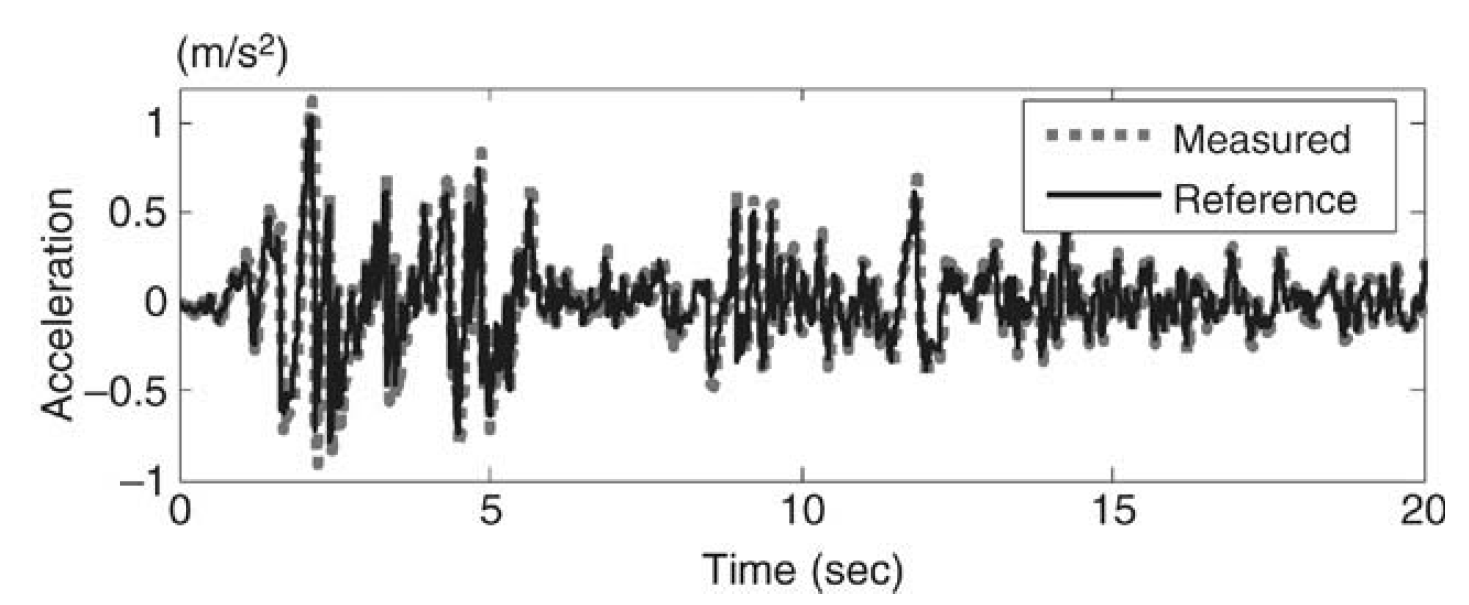
\includegraphics[width=0.8\textwidth] {figure/2-9.png}
\caption{Compensation result for the dynamic characteristic of shaking table}
\label{fig:2-9}
\end{figure}






\subsection{Experimental System for Hybrid Testing of Building with TLD}
\subsubsection{Experimental setup}

In order to experimentally verify the hybrid testing method, an experimental system shown in Figure~\ref{fig:3-2} was set up in Seismic Retrofitting \& Remodeling Research Center at the Dankook University, Seoul, Korea. The TLD was uniaxially excited by the shaking table on which it was mounted. The shear-type load-cell was inserted between the TLD and the shaking table to measure the base shear force yielded by the horizontal motion of the TLD during the test. Also, an accelerometer was attached to the shaking table to monitor its motion.

\begin{figure}[ht]
\centering
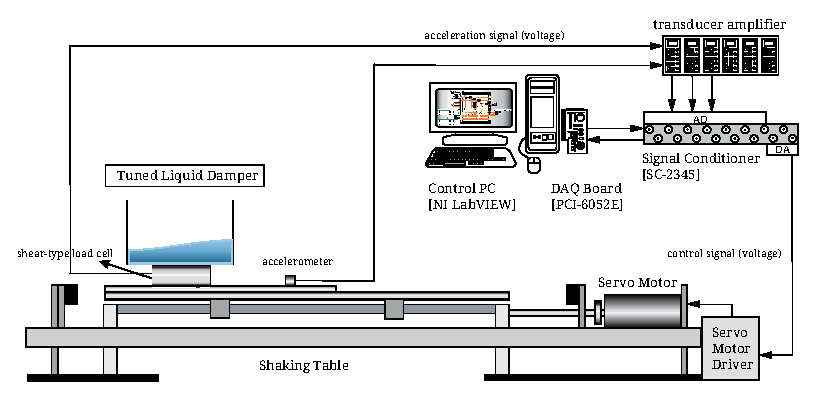
\includegraphics[scale =1] {figure/3-2.eps}
\caption{Schematic diagram of experimental set-up}
\label{fig:3-2}
\end{figure}

\subsubsection{Integrated Controller of the Numerical Structural Model and the Shaking Table}
The numerical structural model and the shaking table dynamics discussed in the previous subsections are integrated into the controller to implement the hybrid testing method. Figure~\ref{fig:3-3} illustrates the block diagram of the hybrid testing method. In the figure, the absolute acceleration is produced by the numerical structural model of Eq.~\eqref{eq:3-3} with two inputs of the measured interacting force, $i_{e}(t)$, and not the measured but the prescribed earthquake record signal, $\ddot{z}_{0}(t)$, as marked by the shaded area. The motion of the shaking table is driven by the controller using the inverse transfer function to minimize the error between the absolute acceleration, $\ddot{Y}_{n}(t)$, calculated as the top story response of the structure and the actual shaking table acceleration, $\ddot{Y}_{e}(t)$. Accordingly, the shaking table itself behaves as the top story of the structure, at which a TLD is installed, and excites the upper TLD that should be physically tested.

\begin{figure}[ht]
\centering
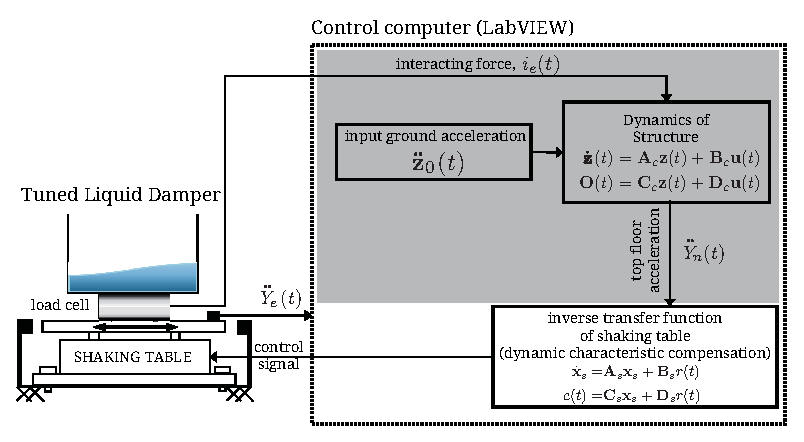
\includegraphics[scale =1] {figure/3-3.eps}
\caption{Block diagram of the integrated controller for the hybrid testing system.}
\label{fig:3-3}
\end{figure}









\subsection{Experimental System for Hybrid Testing of Building with TLCD}
The numerical part and the shaking table controller discussed in previous subsections should be integrated into the controller to implement the hybrid testing shown in Figure~\ref{fig:4-1}. Figure~\ref{fig:4-3} illustrates the block diagram for experimentally implementing the testing method. In the figure, the absolute acceleration is produced by the numerical part such as Eq.~\eqref{eq:4-3} with two inputs of the measured interacting force, $i_{e}(t)$, and not the measured but the prescribed earthquake record signal, $\ddot{z}_{0}(t)$, by a user in the control computer, as marked by the shaded area. The motion of shaking table is driven by the controller using the inverse transfer function to minimize the error between the controlled absolute acceleration, $\ddot{Y}_{n}(t)$, calculated as the top story response of structure and the actual shaking table acceleration, $\ddot{Y}_{e}(t)$. Accordingly, the shaking table itself behaves as the top story of structure, at which a TLCD is installed, and excites the upper TLCD that should be physically tested.
To verify the hybrid testing method, firstly the conventional TLCD-structure interaction model shown in Figure~\ref{fig:4-4a} is experimentally implemented. Then, the hybrid test is shown in Figure~\ref{fig:4-4b}, which the structural model in Figure~\ref{fig:4-4a} is incorporated in the numerical calculation of its identified damping and stiffness coefficients and measured mass, is performed for the controlled case. Finally, two results from controlled cases are compared for the experimental verification of the hybrid testing method.

\begin{figure}[ht]
\centering
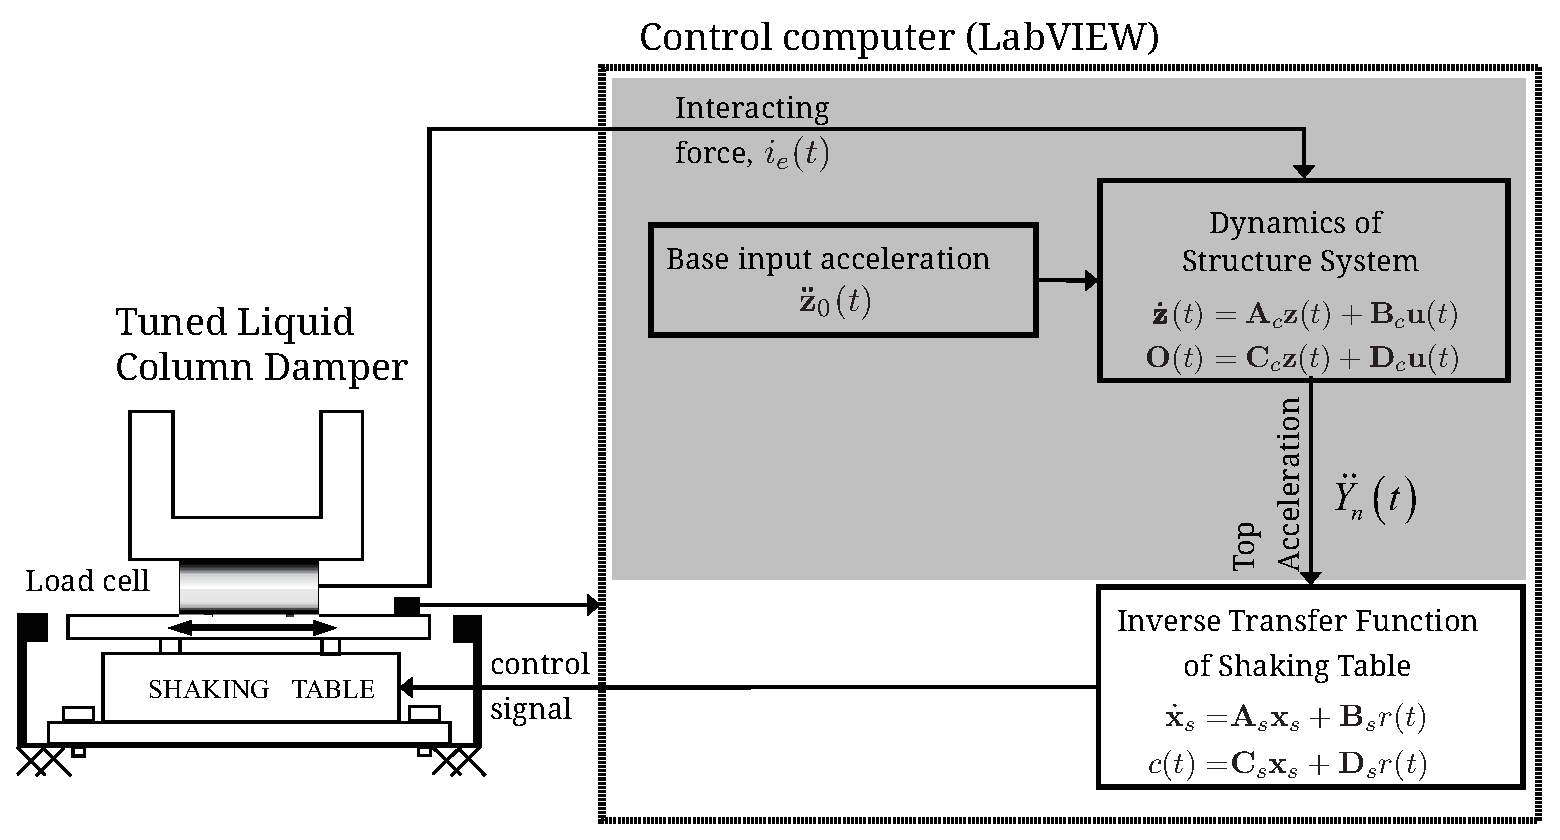
\includegraphics[width=1\textwidth] {figure/4-3.eps}
\caption{Controller for implementing the hybrid testing method}
\label{fig:4-3}
\end{figure}

The only shear-type structural model without the upper TLCD shown in Figure~\ref{fig:4-4a} has the $0.6m$ and $1.0m$ of width and height and $169.7kg$ of measured floor mass. Two records of El Centro and Kobe earthquake waves were excited by the shaking table to measure the absolute structural acceleration. The identification was conducted with measured accelerations of the structure model and the shaking table. The identified parameters have slight differences according to input earthquake waves. The averaged damping, and stiffness coefficients were determined by $14.6N\cdot s/m$ and $9914.3N/m$, respectively, which correspond to $1.23Hz$ of structural natural frequency. The level of water in a TLCD tank was adjusted to sympathize the TLCD frequency to this identified structural one.

\begin{figure}[!ht]
\centering
\subfigure[conventional testing method]{
   \includegraphics[width=0.8\textwidth] {figure/4-4a.eps}
   \label{fig:4-4a}
 }
 \subfigure[hybrid testing method]{
   \includegraphics[width=0.8\textwidth] {figure/4-4b.eps}
   \label{fig:4-4b}
 }
\caption{Experimental view of a building with a TLCD}
\label{fig:4-4}
\end{figure}





\clearpage
\subsection{Experimental System for Hybrid Testing of Building with TLMD}

The difference between the conventional test method and hybrid testing method is that the upper TLMD is adopted as the experimental part, while the structural model is numerically calculated by a computer in the hybrid testing method, as shown in Figure~\ref{fig:5-12}. The control force acting between their interfaces is measured with a shear-type load cell which is mounted on the shaking table. Then, the measured force is fed-back to the numerical analysis part. Finally, the shaking table vibrates the upper experimental part with the responses calculated from the numerical analysis part.

In this case, the shaking table is moved by the control signal sent from the control computer through DA channel of DAQ board. The amplitude and phase of the signal values measured at the shaking table, however, are different from the control signal sent from the control computer. In this paper, the inverse transfer function of a shaking table was designed through the definition of the transfer function of a shaking table, as shown in Figure~\ref{fig:5-13}. Then, a white-noise excitation test of the shaking table is carried out to compensate the dynamic characteristics between the shaking table and control signals, as shown in Figure~\ref{fig:5-14}. 

Figure~\ref{fig:2-7} shows the inverse transfer function of the shaking table which was measured by the acceleration signal as an input data and the command signal as an output data. The measured inverse transfer function of the shaking table could be approximated by using a fifth-order linear filter represented by


\begin{figure}[ht]
\centering
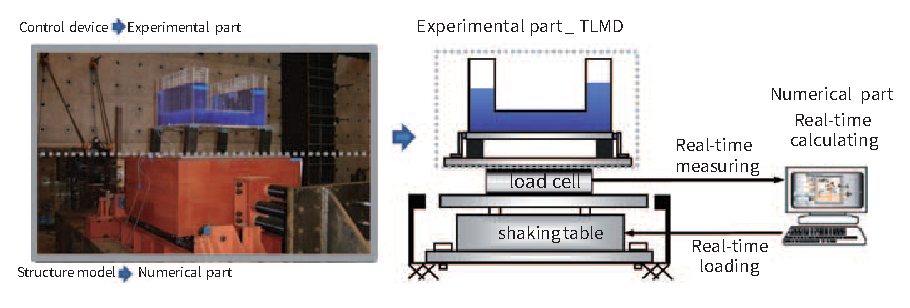
\includegraphics[width=0.8\textwidth] {figure/5-12.eps}
\caption{Conceptual view of the hybrid testing method of building with TLMD}
\label{fig:5-12}
\end{figure}




\subsubsection{Experimental setup}

The SDOF structure subjected to both the external and control forces is given by

\begin{equation}\label{eq:5-7}
m\ddot{x}+c\dot{x}+kx = F(t) - i(t)
\end{equation}

where $m$, $c$ and $k$ are the mass, damping coefficient and stiffness of the SDOF structure, respectively. $F(t)$ and $i(t)$ are the excitation force and TLMD control force measured at the load cell, respectively.

The state-space equation and the output equation for the absolute acceleration of the SDOF structural model such as Eq.~\eqref{eq:5-7} are represented by

\begin{align}
\dot{\matr{z}}&=\matr{A}\matr{z}+\matr{B}u \label{eq:5-8} \\
\bar{y_{1}}&=\matr{C}\matr{z} + \matr{D}u \label{eq:5-9}
\end{align}

where $z$ and $u$ are state variable and input vector, and can be expressed as $\matr{z}=\left[x, \dot{x}\right]^{\top}$ and $\matr{u} = \left[i(t), F(t)\right]^{\top}$, respectively. $\bar{y}_{1}$ is the absolute acceleration of the SDOF structural model, and the matrices $\matr{A}$, $\matr{B}$, $\matr{C}$ and $\matr{D}$ are follow-up as Eqs.~\eqref{eq:5-10}-\eqref{eq:5-13}, respectively.

\begin{align}
\matr{A}&=\begin{bmatrix} 0 & 1 \\ -k/m & -c/m \end{bmatrix} \label{eq:5-10} \\
\matr{B}&=\begin{bmatrix} 0 & 0 \\ -1/m & 1/m \end{bmatrix} \label{eq:5-11} \\
\matr{C}&=\begin{bmatrix} -k/m & -c/m \end{bmatrix} \label{eq:5-12} \\
\matr{D}&=\begin{bmatrix} -1/m & 1/m \end{bmatrix} \label{eq:5-13}
\end{align}

Finally, the controller both considering the numerical part of the SDOF structural model and the inverse transfer function of a shaking table is constructed to implement the hybrid testing method as shown in Figure~\ref{fig:5-16}. Figure~\ref{fig:5-17} shows the experimental configuration of the test. The hybrid testing method is fatal to the noise and phase error because the shaking table is vibrated by the numerical part which is calculated in real-time. Accordingly, the hybrid test using the Real-Time Window Target of the MATLAB Simulink with the sampling rate of 1000 Hz was implemented to minimize the calculation and phase error in the actual test. Figure~\ref{fig:5-18} is an excitation model of the Real-Time Window Target of the MATLAB Simulink, and it includes the inverse transfer function of the shaking table and numerical analysis of the SDOF structure.

\begin{figure}[ht]
\centering
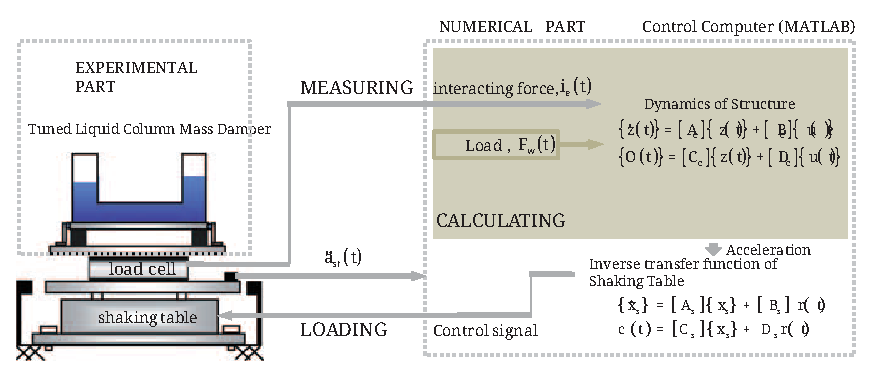
\includegraphics[width=0.8\textwidth] {figure/5-16.eps}
\caption{Design of the controller for the hybrid testing method}
\label{fig:5-16}
\end{figure}

\begin{figure}[ht]
\centering
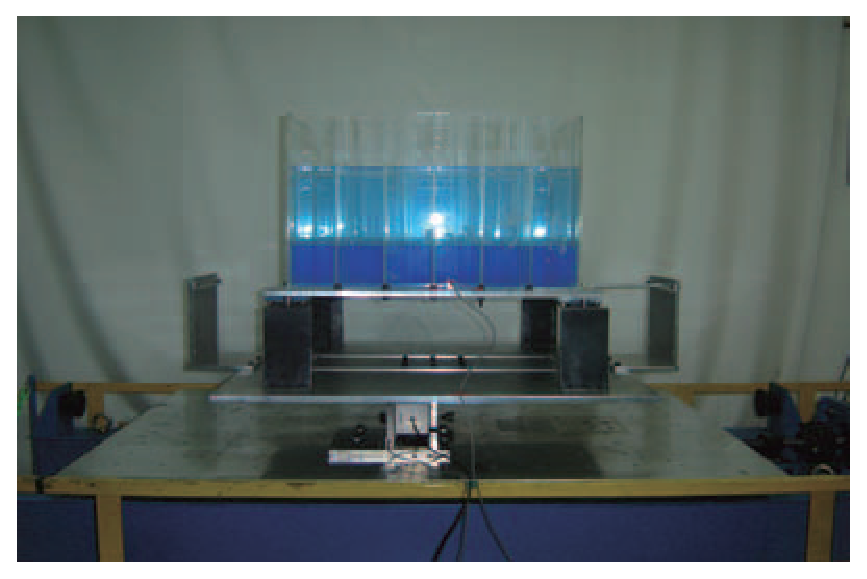
\includegraphics[width=0.8\textwidth] {figure/5-17.eps}
\caption{Photograph of the hybrid testing}
\label{fig:5-17}
\end{figure}

\begin{figure}[ht]
\centering
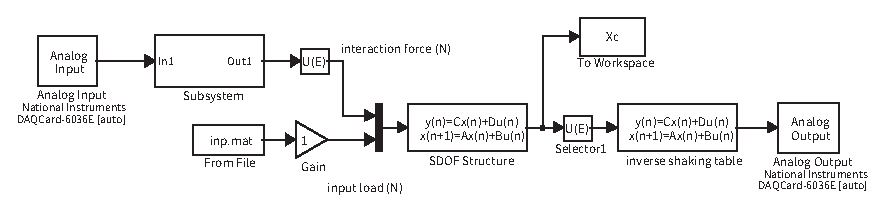
\includegraphics[width=0.8\textwidth] {figure/5-18.eps}
\caption{Design of the MATLAB Simulink window Target}
\label{fig:5-18}
\end{figure}








\clearpage

%\part{Experimantal Implementation}
\section{Experimental Verification}
\subsection{Experimental result of Substructuring technique}

The validity of the proposed substructuring technique as part of the hybrid testing method is verified for the experimental setting described in the previous sections. First, the shaking table test without feedback loop of accelerations measured from the experimental substructure into the shaking table controller in Figure~\ref{fig:2-11} is performed to confirm the validity of the proposed method experimentally. In this case, the third story acceleration of responses pre-calculated from the assumed whole building with structural parameters such as Eqs.~\eqref{eq:2-18} and \eqref{eq:2-19} is used as a reference signal in Figure~\ref{fig:2-8}. Figure~\ref{fig:2-12} compares the time histories and Fourier transform of the acceleration responses, which are measured from the experimental substructure and shaking table, with those calculated from the numerical analysis of the whole assumed structure. In other words, the responses corresponding to the 3rd, 4th and 5th story accelerations are compared. Also, Figures~\ref{fig:2-13}-\ref{fig:2-15} showing the variation of frequency components according to time lapse illustrate the spectrogram and contour plots of experimental and numerical accelerations of the 3rd, 4th and 5th story, respectively. As can be confirmed from Figure~\ref{fig:2-12}, the experimental accelerations obtained from the shaking table test without their feedback agree well with those obtained from the analysis of the whole assumed structure in both time and frequency domains. However, it can be observed that the small discrepancies are shown in the time histories of 4th and 5th story accelerations as shown from Figure~\ref{fig:2-12}, while the 3rd story acceleration is identical to the numerical one over the entire time history as known from Figures~\ref{fig:2-12}-\ref{fig:2-13}. These differences are caused by the inherent modes of experimental substructure; the frequency components of 2.5 and 8.6 Hz corresponding to the first and second modes of the experimental substructure, respectively, are observed in the measured acceleration of 4th story as known from Figure~\ref{fig:2-14}, and also the component of 2.5 Hz is expressed in the 5th story experimental acceleration as like Figure~\ref{fig:2-15}. It is considered that this tendency is especially conspicuous in the case of utilizing a lightly-damped testing model as an experimental substructure. Table 1 shows the frequency components observed in the time records of an experimental substructure from the test without its acceleration feedback and the natural frequencies calculated from the whole assumed structure with five stories. From Table~\ref{tab:2-1}, it can be noted that the first natural frequency of the experimental substructure is shifted from 2.5 Hz to 1.3 Hz by the dynamics of the three-story numerical substructure added to its base.
 Then, the substructuring testing expressed as Figure~\ref{fig:2-11} was carried out based on the acceleration feedback of the experimental substructure. Figure~\ref{fig:2-16} compares the responses measured by the test with the acceleration feedback of the experimental substructure with those calculated from the numerical analysis of the whole assumed structure with 5 DOFs. Also, Figures~\ref{fig:2-17}-\ref{fig:2-19} express the frequency components according to time lapse, which is observed in the measured responses from the test with feedback and the calculated ones of the 3rd, fourth and fifth story, respectively. As known from Figure~\ref{fig:2-16}, the inclination in entire time history responses measured from the proposed testing method agrees well with that calculated from the whole assumed structure. These are why the first mode responses of substructured system coincide well with those of the whole supposed system over the entire time range, as shown in Figures~\ref{fig:2-17}-\ref{fig:2-19}. However, as can be confirmed from Figures~\ref{fig:2-17}-\ref{fig:2-19}, instead of the second and third mode responses of the substructured system, those of the experimental substructure are observed from the testing results in the vicinity of 2.5 and 8.6 Hz. It is considered that in the process of the acceleration feedback of the experimental substructure, its fundamental modes affect to the numerical substructure and then the numerical error occurs in calculating the numerical substructure.

\begin{figure}[ht]
\centering
\subfigure[Time domain]{
   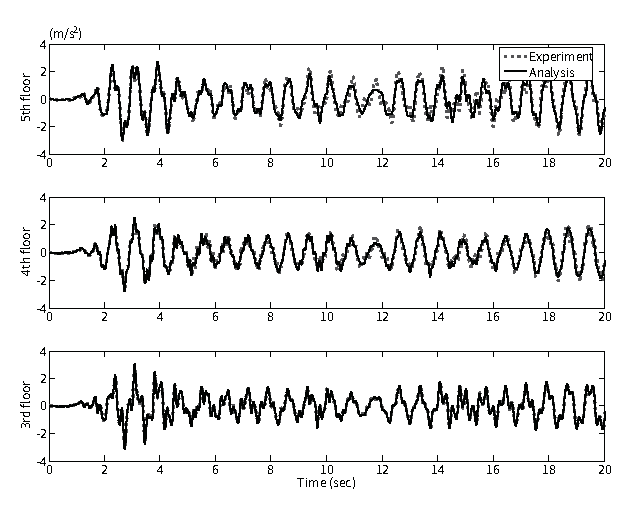
\includegraphics[width=0.8\textwidth] {figure/2-12a.eps}
   \label{fig:2-12a}
 }
 \subfigure[Frequency domain]{
   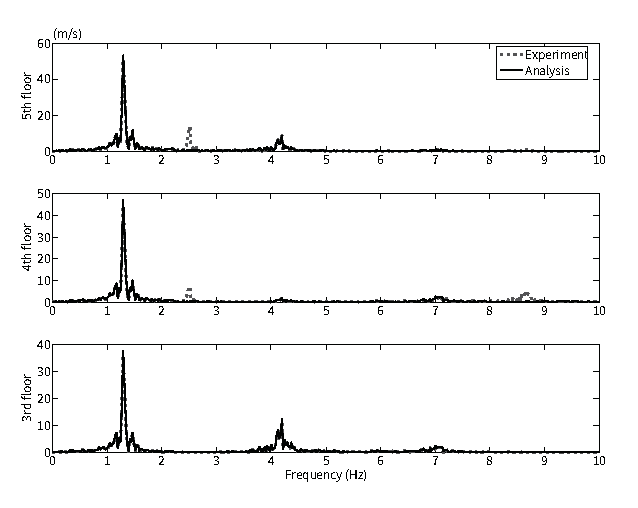
\includegraphics[width=0.8\textwidth] {figure/2-12b.eps}
   \label{fig:2-12b}
 }
\caption{Comparisons of results measured from the experiment without feedback and those calculated from numerical analysis.}
\label{fig:2-12}
\end{figure}

\begin{figure}[ht]
\centering
 \subfigure[Spectrogram of the response measured from the experiment without feedback]{
   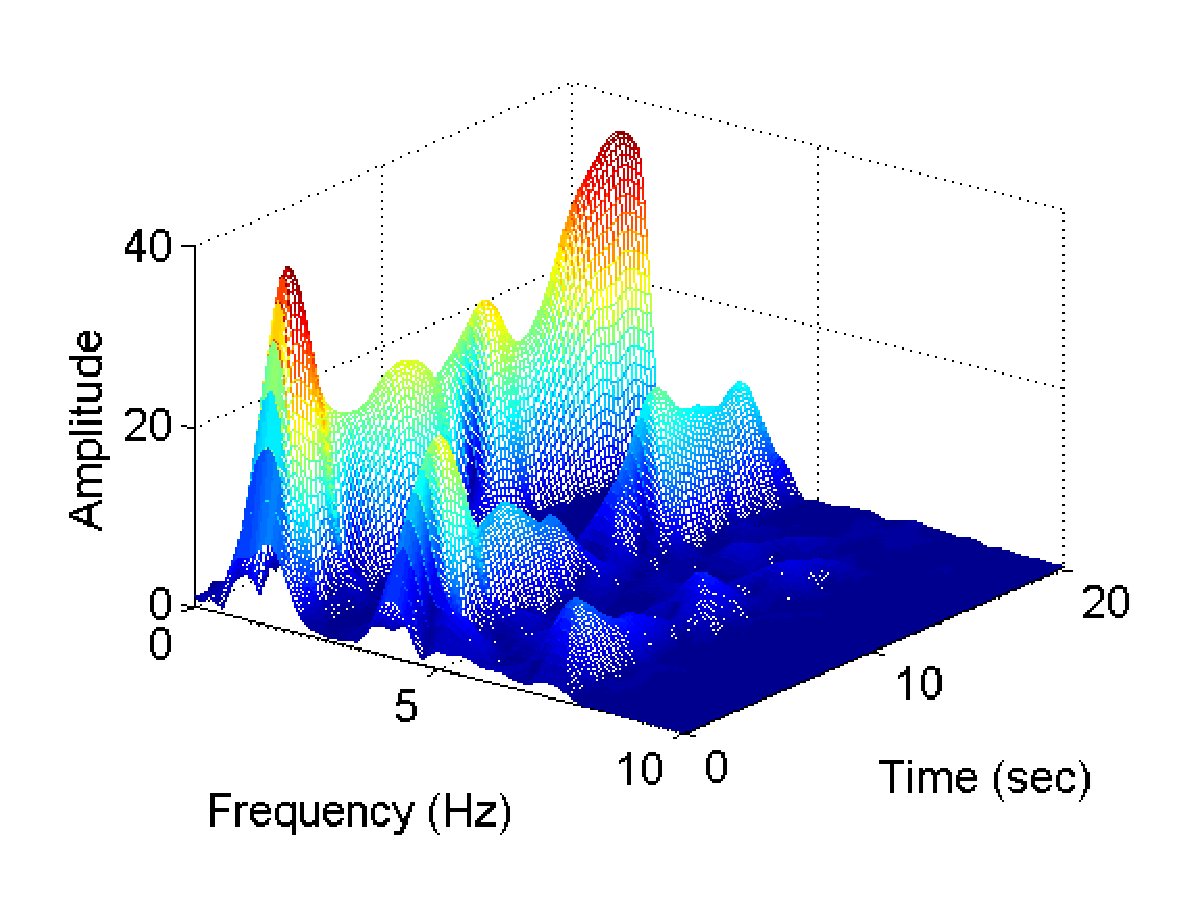
\includegraphics[width=0.45\textwidth] {figure/2-13a.eps}
   \label{fig:2-13a}
 }\hfill
 \subfigure[Spectrogram of the response calculated from the numerical analysis measured]{
   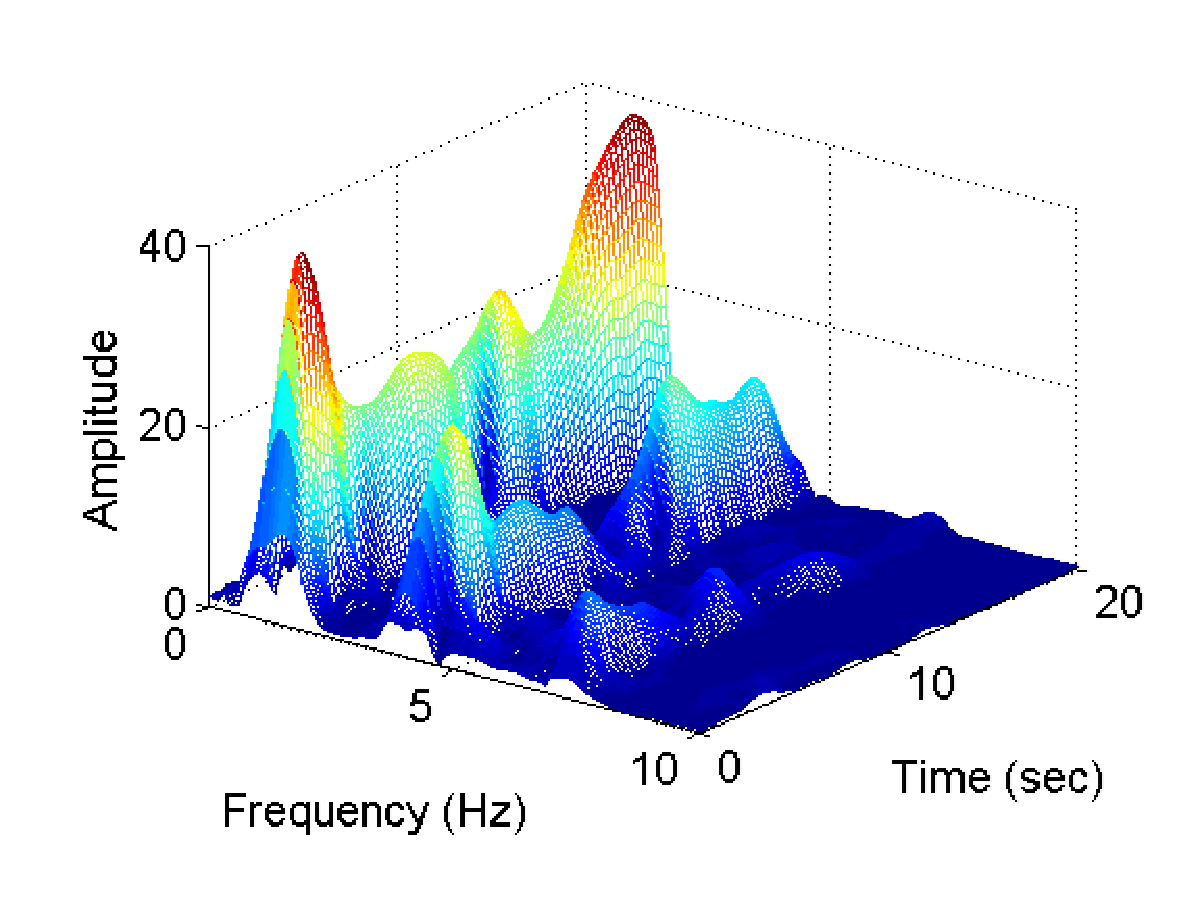
\includegraphics[width=0.45\textwidth] {figure/2-13b.eps}
   \label{fig:2-13b}
 }
 \subfigure[Contour plot of the response measured from the experiment without feedback]{
   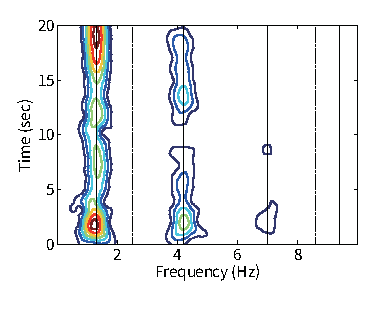
\includegraphics[width=0.45\textwidth] {figure/2-13c.eps}
   \label{fig:2-13c}
 }\hfill
 \subfigure[Contour plot of the response calculated from the numerical analysis measured]{
   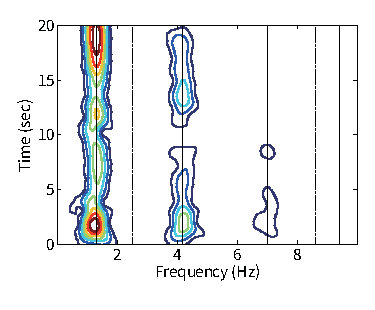
\includegraphics[width=0.45\textwidth] {figure/2-13d.eps}
   \label{fig:2-13d}
 }
\caption{Spectrograms and contour plots of the 3rd story acceleration measured from the experiment without feedback and that calculated from the numerical analysis.}
\label{fig:2-13}
\end{figure}

\begin{figure}[ht]
\centering
 \subfigure[Spectrogram of the response measured from the experiment without feedback]{
   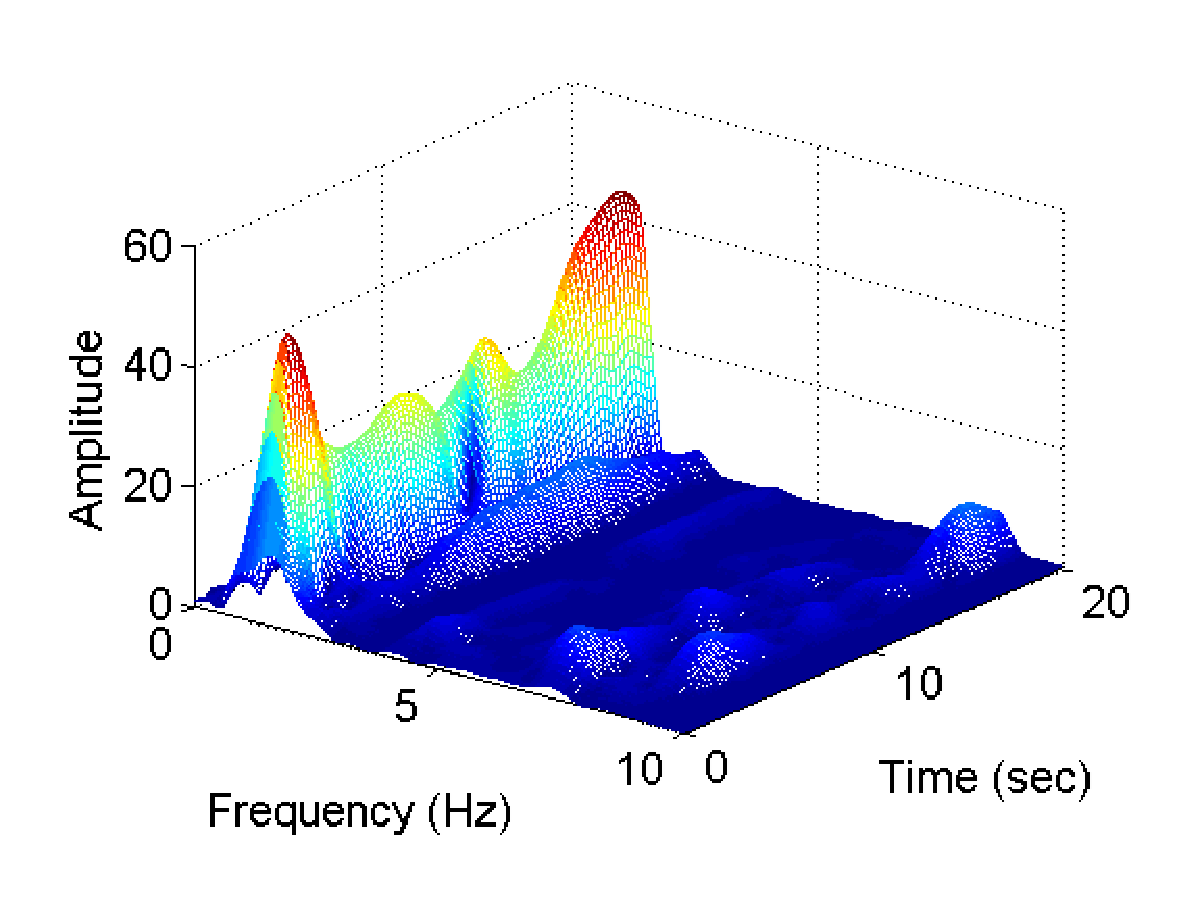
\includegraphics[width=0.45\textwidth] {figure/2-14a.eps}
   \label{fig:2-14a}
 }\hfill
 \subfigure[Spectrogram of the response calculated from the numerical analysis measured]{
   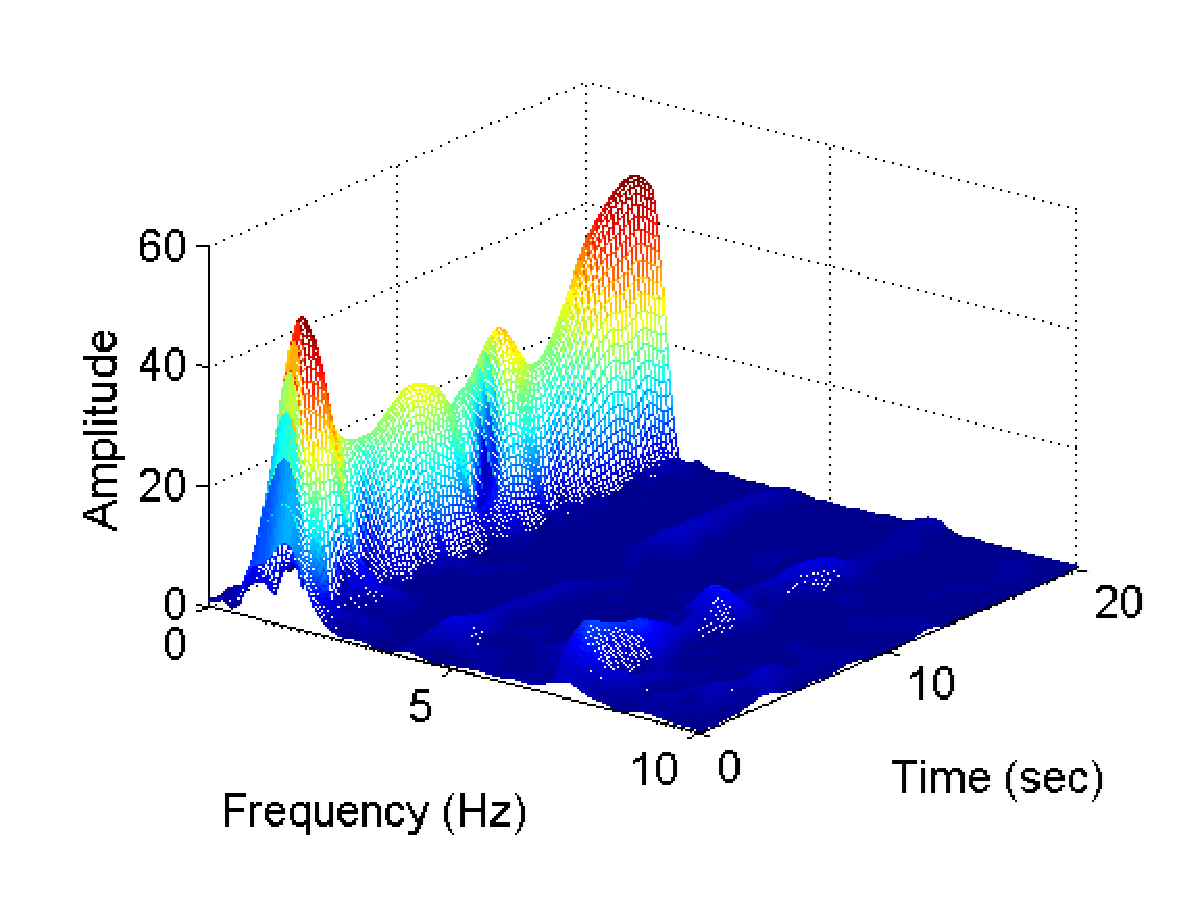
\includegraphics[width=0.45\textwidth] {figure/2-14b.eps}
   \label{fig:2-14b}
 }
 \subfigure[Contour plot of the response measured from the experiment without feedback]{
   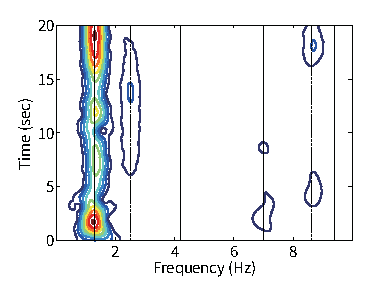
\includegraphics[width=0.45\textwidth] {figure/2-14c.eps}
   \label{fig:2-14c}
 }\hfill
 \subfigure[Contour plot of the response calculated from the numerical analysis measured]{
   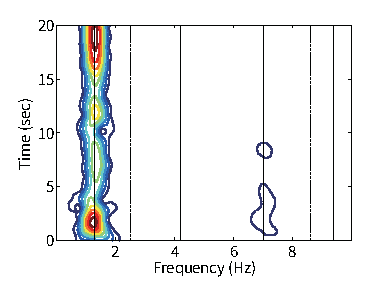
\includegraphics[width=0.45\textwidth] {figure/2-14d.eps}
   \label{fig:2-14d}
 }
\caption{Spectrograms and contour plots of the 4th story acceleration measured from the experiment without feedback and that calculated from the numerical analysis.}
\label{fig:2-14}
\end{figure}

\begin{figure}[ht]
\centering
 \subfigure[Spectrogram of the response measured from the experiment without feedback]{
   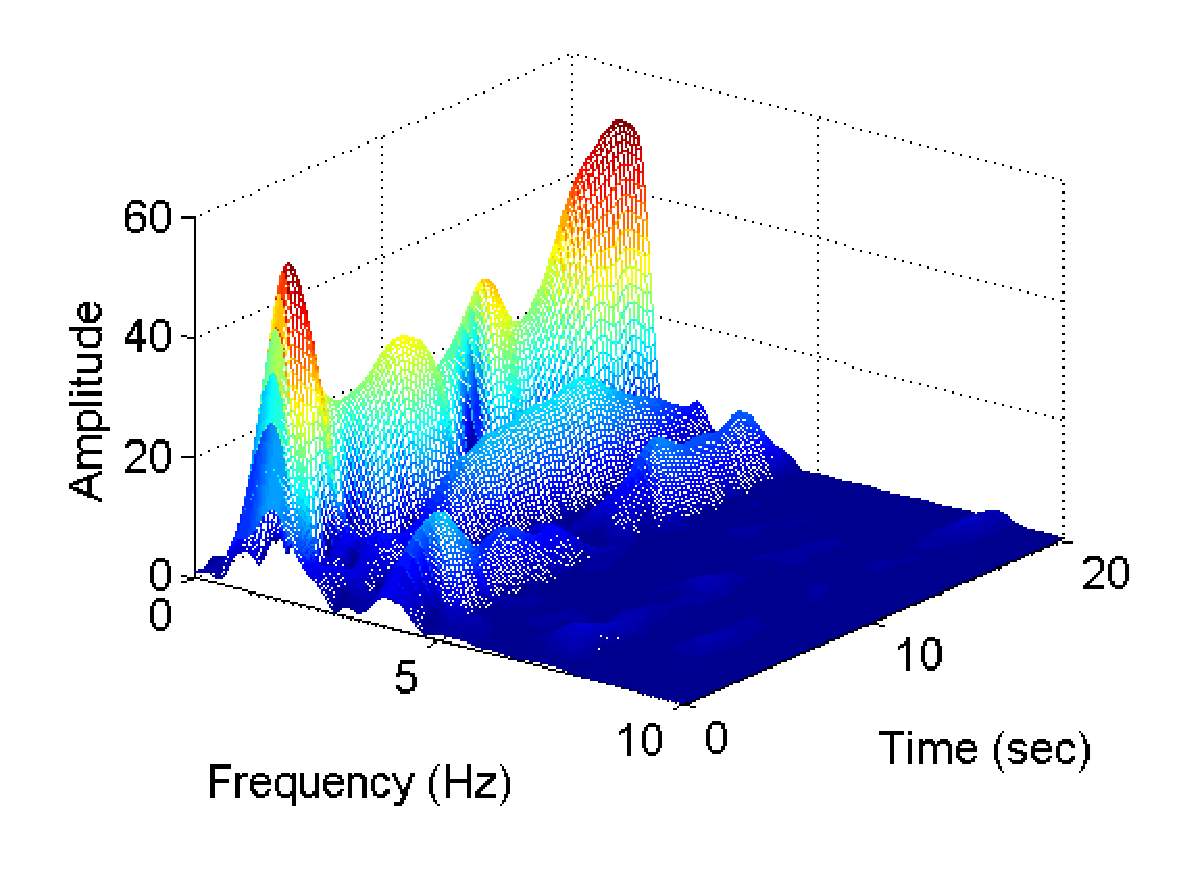
\includegraphics[width=0.45\textwidth] {figure/2-15a.eps}
   \label{fig:2-15a}
 }\hfill
 \subfigure[Spectrogram of the response calculated from the numerical analysis measured]{
   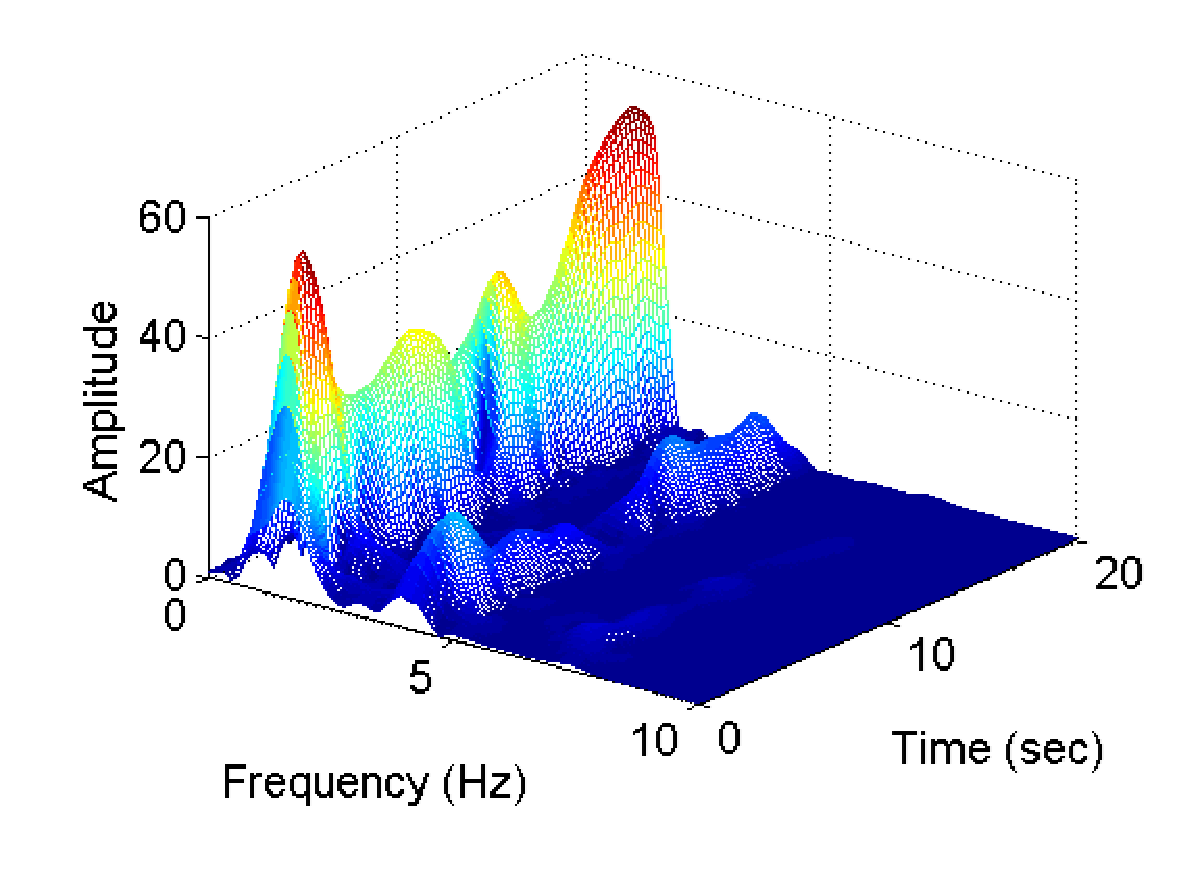
\includegraphics[width=0.45\textwidth] {figure/2-15b.eps}
   \label{fig:2-15b}
 }
 \subfigure[Contour plot of the response measured from the experiment without feedback]{
   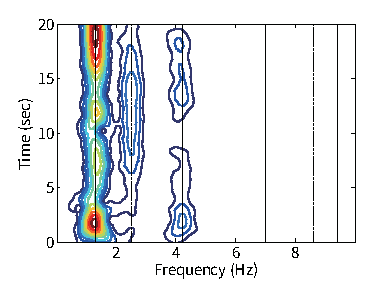
\includegraphics[width=0.45\textwidth] {figure/2-15c.eps}
   \label{fig:2-15c}
 }\hfill
 \subfigure[Contour plot of the response calculated from the numerical analysis measured]{
   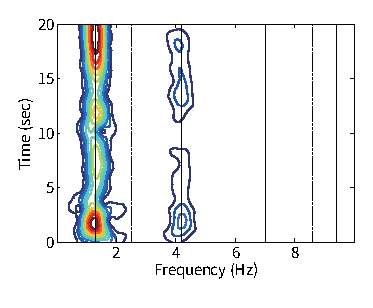
\includegraphics[width=0.45\textwidth] {figure/2-15d.eps}
   \label{fig:2-15d}
 }
\caption{Spectrograms and contour plots of the 5th story acceleration measured from the experiment without feedback and that calculated from the numerical analysis.}
\label{fig:2-15}
\end{figure}

\begin{figure}[ht]
\centering
\subfigure[Time domain]{
   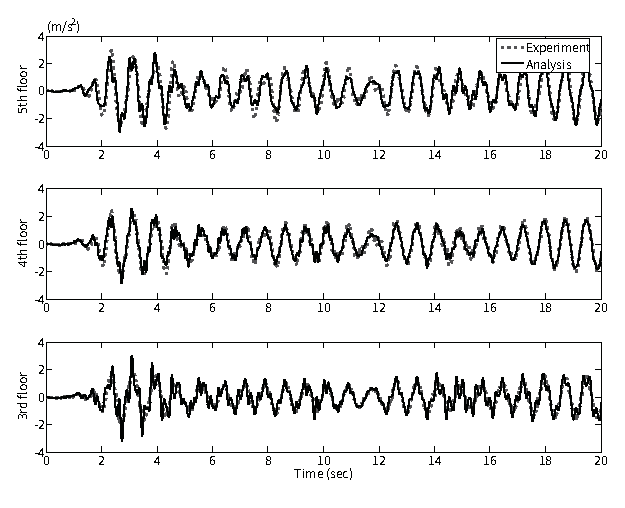
\includegraphics[width=0.8\textwidth] {figure/2-16a.eps}
   \label{fig:2-16a}
 }
 \subfigure[Frequency domain]{
   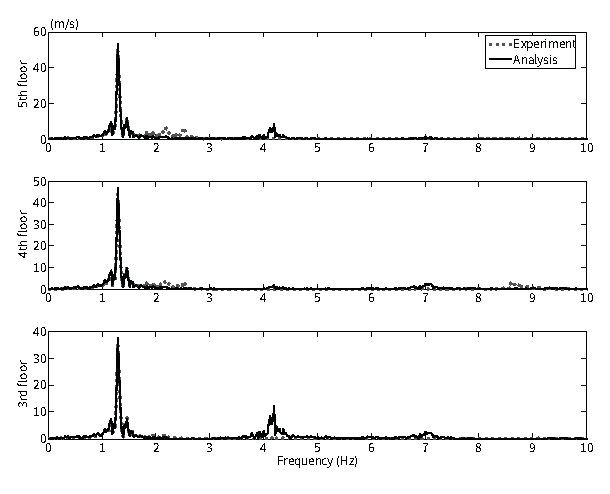
\includegraphics[width=0.8\textwidth] {figure/2-16b.eps}
   \label{fig:2-16b}
 }
\caption{Comparisons between results from the experiment with feedback and those from analysis.}
\label{fig:2-16}
\end{figure}

\begin{figure}[ht]
\centering
 \subfigure[Spectrogram of the response measured from the experiment without feedback]{
   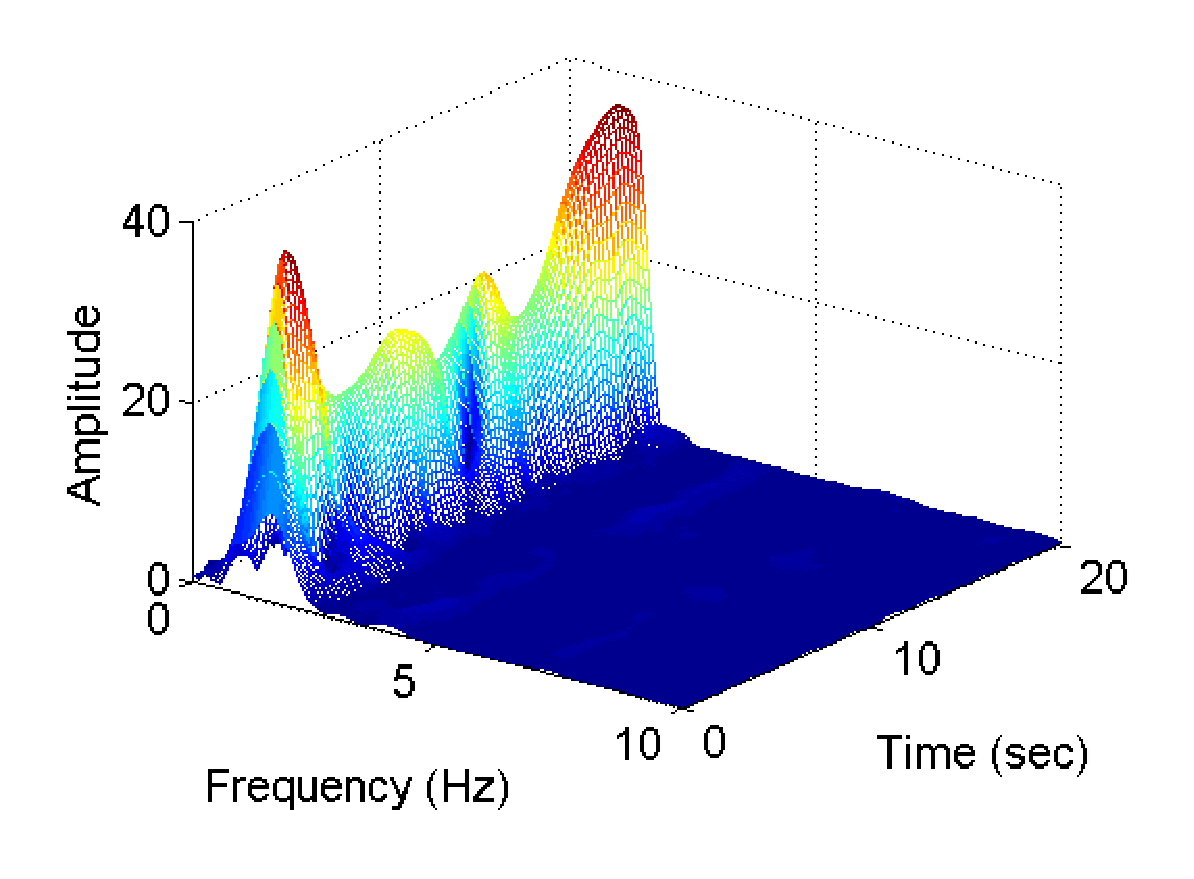
\includegraphics[width=0.45\textwidth] {figure/2-17a.eps}
   \label{fig:2-17a}
 }\hfill
 \subfigure[Spectrogram of the response calculated from the numerical analysis measured]{
   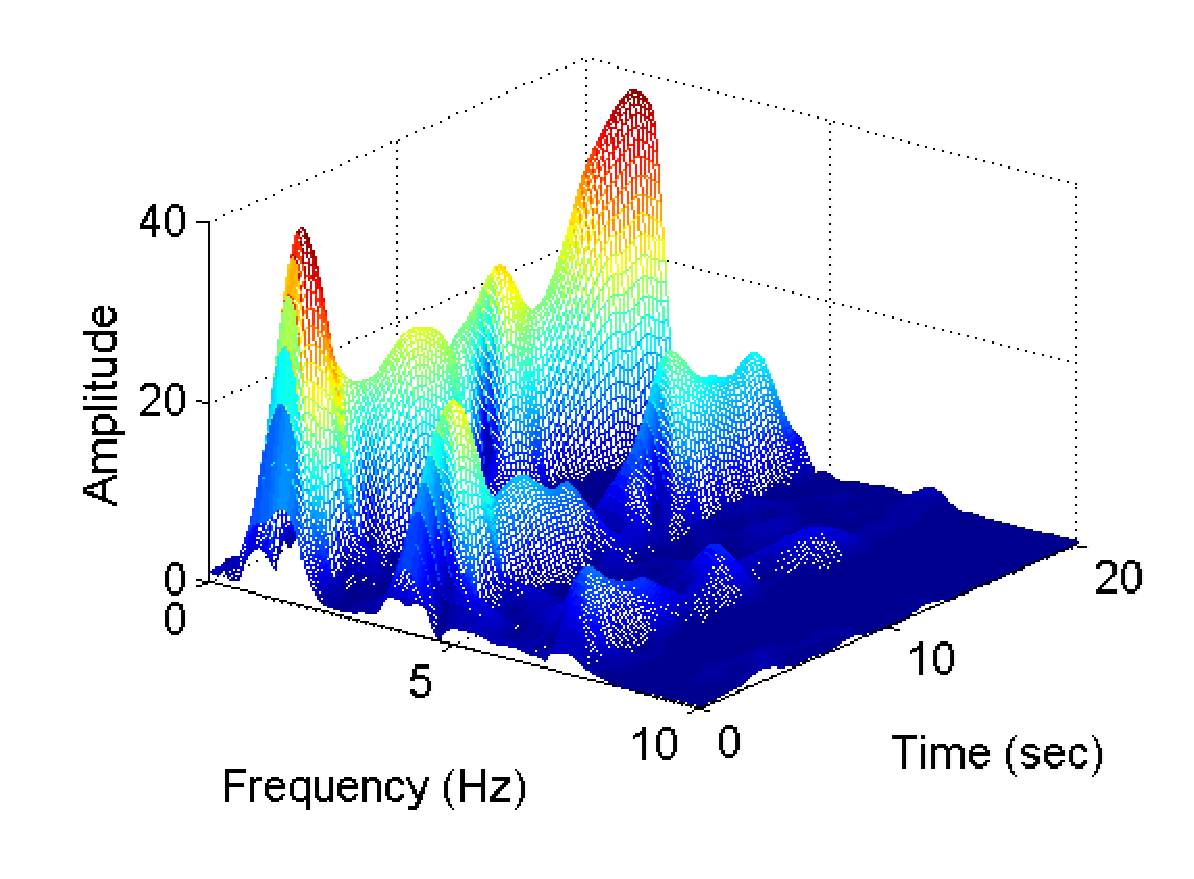
\includegraphics[width=0.45\textwidth] {figure/2-17b.eps}
   \label{fig:2-17b}
 }
 \subfigure[Contour plot of the response measured from the experiment without feedback]{
   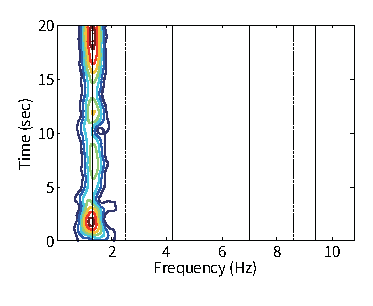
\includegraphics[width=0.45\textwidth] {figure/2-17c.eps}
   \label{fig:2-17c}
 }\hfill
 \subfigure[Contour plot of the response calculated from the numerical analysis measured]{
   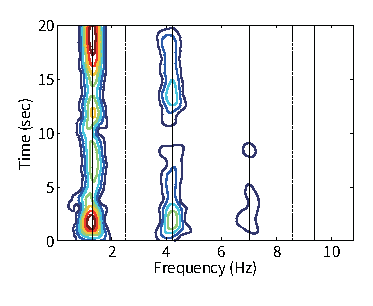
\includegraphics[width=0.45\textwidth] {figure/2-17d.eps}
   \label{fig:2-17d}
 }
\caption{Spectrograms and contour plots of the 3rd story acceleration measured from the experiment with feedback and that calculated from the numerical analysis.}
\label{fig:2-17}
\end{figure}

\begin{figure}[ht]
\centering
 \subfigure[Spectrogram of the response measured from the experiment without feedback]{
   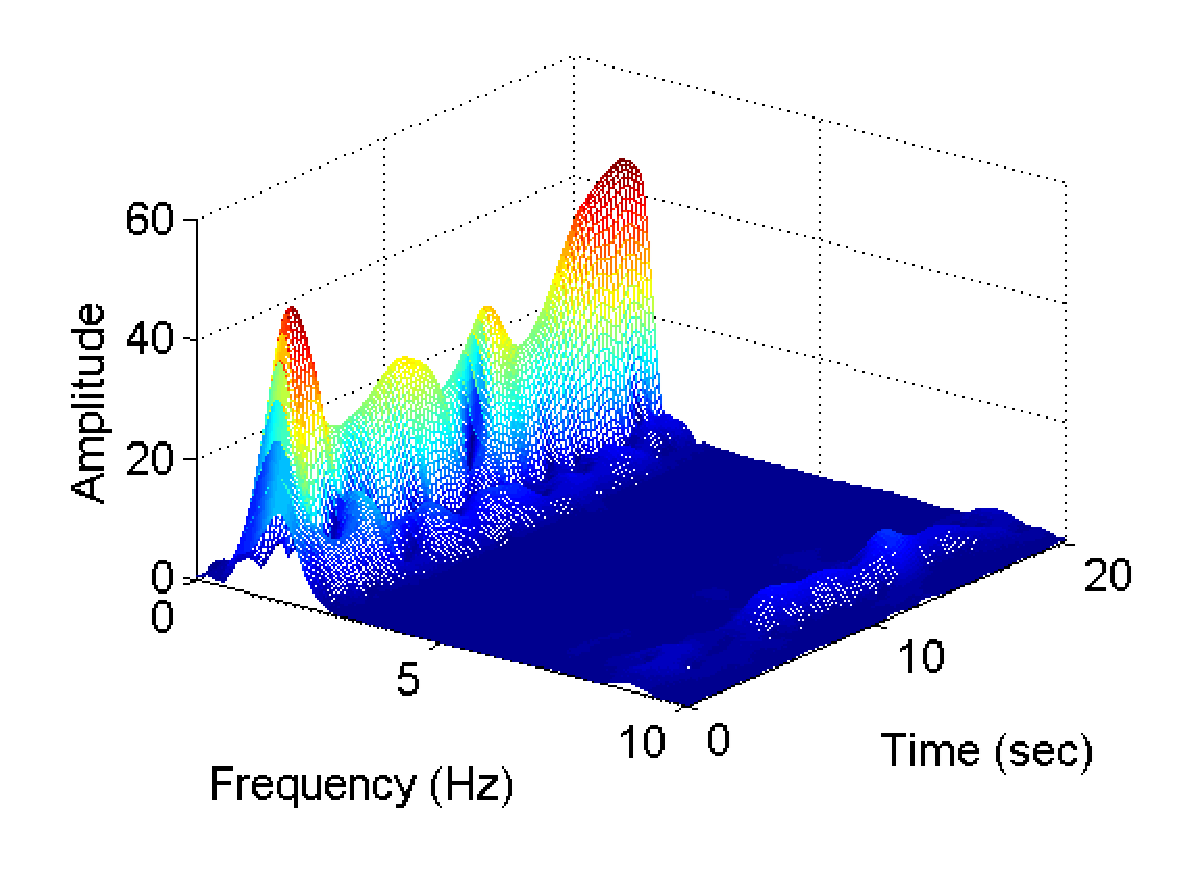
\includegraphics[width=0.45\textwidth] {figure/2-18a.eps}
   \label{fig:2-18a}
 }\hfill
 \subfigure[Spectrogram of the response calculated from the numerical analysis measured]{
   \includegraphics[width=0.45\textwidth] {figure/2-18b.eps}
   \label{fig:2-18b}
 }
 \subfigure[Contour plot of the response measured from the experiment without feedback]{
   \includegraphics[width=0.45\textwidth] {figure/2-18c.eps}
   \label{fig:2-18c}
 }\hfill
 \subfigure[Contour plot of the response calculated from the numerical analysis measured]{
   \includegraphics[width=0.45\textwidth] {figure/2-18d.eps}
   \label{fig:2-18d}
 }
\caption{Spectrograms and contour plots of the 4th story acceleration measured from the experiment with feedback and that calculated from the numerical analysis.}
\label{fig:2-18}
\end{figure}

\begin{figure}[ht]
\centering
 \subfigure[Spectrogram of the response measured from the experiment without feedback]{
   \includegraphics[width=0.45\textwidth] {figure/2-19a.eps}
   \label{fig:2-19a}
 }\hfill
 \subfigure[Spectrogram of the response calculated from the numerical analysis measured]{
   \includegraphics[width=0.45\textwidth] {figure/2-19b.eps}
   \label{fig:2-19b}
 }
 \subfigure[Contour plot of the response measured from the experiment without feedback]{
   \includegraphics[width=0.45\textwidth] {figure/2-19c.eps}
   \label{fig:2-19c}
 }\hfill
 \subfigure[Contour plot of the response calculated from the numerical analysis measured]{
   \includegraphics[width=0.45\textwidth] {figure/2-19d.eps}
   \label{fig:2-19d}
 }
\caption{Spectrograms and contour plots of the 5th story acceleration measured from the experiment with feedback and that calculated from the numerical analysis.}
\label{fig:2-19}
\end{figure}

% \clearpage
% \section{Concluding Remarks}
% In this study, a new real-time substructuring technique for the shaking table test was proposed. The proposed substructuring technique adopts the upper part of the whole structure as the experimental substructure, which corresponds to a physical test model. In order to verify the validity and accuracy of the proposed technique, a shaking table test was conducted. The result of the study can be summarized as follows.
% \begin{enumerate}
% \item To reduce the distortion of the interface acceleration, the inverse transfer function of the shaking table was identified, and its state space realization was implemented in the shaking table controller.
% \item In this paper, the linear transfer function approach for controlling the motion of a shaking table was considered to verify the proposed method for a linear experimental part experimentally. However, this approach would be inappropriate in a coupled non-linear system leading to experimental instability. Therefore, in such case the controller using the inverse transfer function of shaking table, shown in Fig. 11, would be modified to compensate an experimental instability.
% \item The interface force between the experimental and numerical substructures was obtained using only acceleration measurement and mass information so that high-capacity loads cell and installation jigs are not required in the experiment. 
% \item The proposed method basing the interface force measurement on acceleration measurements from an experimental substructure is partially available only when the mass distribution is discrete - for example this would be applicable to the TMD as an experimental part. Also, the interface force measurement using force transducers is required to perform the proposed method when wind forces are applied to the experimental substructure.
% \item Experimental results demonstrate that the proposed real-time substructuring technique can reproduce the dynamic behavior of the whole assumed structure.
% \item Unexpected vibration of the experimental substructure can be induced by the feedback of responses including its inherent natural modes and then by the error occurred in calculating the numerical substructure.
% \item It is considered that to minimize the effect of natural modes of an experimental substructure on the substructured system, the structural model as heavily-damped as possible would be used as an experimental part.
% \item The proposed technique can be extended to the real-time substructuring technique with the middle part of a whole structure in combination with the conventional substructuring technique employing lower part as the experimental substructure.
% \end{enumerate}


\clearpage
\subsection{Hybrid Testing Method of a Single Story Strcuture with a TLD}
In this section, experimental verification of the hybrid testing method is conducted for a single story steel frame with a TLD. First, the conventional TLD-structure interaction model shown in Figure~\ref{fig:3-4a} is tested. Then, the hybrid testing method shown in Figure~\ref{fig:3-4b}, which incorporates the single story steel frame in the numerical calculation, is performed and the results from the two testing methods are compared to each other.
For the numerical structural model used in the hybrid testing method, the single story steel frame is assumed to be an SDOF mass-damping-spring system. The structure has $0.6m$ of width, $1.0m$ of height and $169.7kg$ of measured floor mass. El Centro, Hachinohe, Mexico City, and Northridge earthquake waves were realized by the shaking table, and the resulting absolute accelerations of the floor and the shaking table were measured. The system identification was conducted using the measured absolute accelerations. The identified parameters slightly vary according to input earthquake waves. The averaged damping and stiffness coefficients are 14.6$N\cdot s/m$ and $9914.3N/m$, respectively, which correspond to $1.23Hz$ of structural natural frequency. The TLD shown in Figure~\ref{fig:3-4} has the size of $31(cm)\times14(cm)\times20(cm)$. The level of water in the TLD was adjusted to have $3.4cm$ that is theoretically calculated based on the linear wave theory\citep{soong1997passive} for the TLD to have fundamental sloshing frequency tuned to the identified structural natural frequency. As a result, the mass ratio of the TLD to the structure is about $1.3\%$. To confirm whether the numerically calculated frequency of the TLD is modulated to the structural one, the transfer function is shown in Figure~\ref{fig:3-5}, from the shaking table acceleration to the shear force by the TLD, was obtained by using the white noise excitation. It is observed in Figure~\ref{fig:3-5} that the TLD has the sloshing frequency of $1.25Hz$ which is very close to the structural natural frequency of $1.23Hz$.

\begin{figure}[!ht]
\centering
\subfigure[Conventional shaking table test]{
   \includegraphics[width=0.8\textwidth] {figure/3-4a.eps}
   \label{fig:3-4a}
 }
 \subfigure[Hybrid shaking table test]{
   \includegraphics[width=0.8\textwidth] {figure/3-4b.eps}
   \label{fig:3-4b}
 }
\caption{TLD-structure interaction experimental system.}
\label{fig:3-4}
\end{figure}

\begin{figure}[!ht]
\centering
\includegraphics[width=0.8\textwidth] {figure/3-5.eps}
\caption{TLD transfer function from the table acceleration to the base shear force}
\label{fig:3-5}
\end{figure}

At first, the conventional shaking table test is shown in Figure~\ref{fig:3-4a} is performed to investigate the seismic response control performance of the TLD. Previously mentioned four earthquake records are scaled to have the peak acceleration of 100 gals and used to excite the TLD-structure system. Figures~\ref{fig:3-6} and \ref{fig:3-7} show the measured structural acceleration responses in the time and frequency domains, respectively. It is observed from Figure~\ref{fig:3-6} that acceleration in the latter part of the whole response history is significantly reduced. This phenomenon is a common tendency in the structural response controlled by a tuned mass-type control device since it makes an effect when the structural response is governed by the fundamental mode after initial high impulse like component has passed. In response to Mexico-city earthquake excitation, as shown in Figure~\ref{fig:3-7c}, the first peak corresponding to the major frequency component of the earthquake itself is not controlled, but the response in the region of the TLD modulation frequency is reduced to nearly zero.

\begin{figure}[!ht]
\centering
 \subfigure[El Centro earthquake]{
   \includegraphics[width=0.8\textwidth] {figure/3-6a.eps}
   \label{fig:3-6a}
 }
 \subfigure[Hachinohe earthquake]{
   \includegraphics[width=0.8\textwidth] {figure/3-6b.eps}
   \label{fig:3-6b}
 }
 \subfigure[Mexico city earthquake]{
   \includegraphics[width=0.8\textwidth] {figure/3-6c.eps}
   \label{fig:3-6c}
 }
 \subfigure[Northridge earthquake]{
   \includegraphics[width=0.8\textwidth] {figure/3-6d.eps}
   \label{fig:3-6d}
 }
\caption{Structural acceleration in the time domain measured from the conventional shaking table test of TLD-structure interaction system (dotted line : without control, solid line : with control)}
\label{fig:3-6}
\end{figure}

\begin{figure}[!ht]
\centering
 \subfigure[El Centro earthquake]{
   \includegraphics[width=0.45\textwidth] {figure/3-7a.eps}
   \label{fig:3-7a}
 }\hfill
 \subfigure[Hachinohe earthquake]{
   \includegraphics[width=0.45\textwidth] {figure/3-7b.eps}
   \label{fig:3-7b}
 }
 \subfigure[Mexico city earthquake]{
   \includegraphics[width=0.45\textwidth] {figure/3-7c.eps}
   \label{fig:3-7c}
 }\hfill
 \subfigure[Northridge earthquake]{
   \includegraphics[width=0.45\textwidth] {figure/3-7d.eps}
   \label{fig:3-7d}
 }
\caption{Structural acceleration in the frequency domain measured from the conventional shaking table test of TLD-structure interaction system (dotted line : without control, solid line : with control)}
\label{fig:3-7}
\end{figure}

Then, the hybrid testing method is applied with the experimental set-up shown in Figure~\ref{fig:3-4b}. For its implementation for the controlled case, the identified structural parameters are reflected in the numerical part expressed by the shaded region in the integrated controller shown in Figure~\ref{fig:3-3}. The continuous filters are converted into discrete ones with a time interval of 0.01 second. Figures~\ref{fig:3-8} and \ref{fig:3-9} compare the controlled accelerations obtained by performing the conventional and the hybrid testing method in time and frequency domains, respectively. The effectiveness of the hybrid testing method is verified by the fact that the experimental results from two methods coincide well with each other on the whole. The small discrepancies existing in the controlled responses subjected to El Centro and Hachinohe earthquakes are considered to result from the underestimation of damping coefficients in the numerical structural model since averaged parameters for the four earthquake data were used.

\begin{figure}[!ht]
\centering
 \subfigure[El Centro earthquake]{
   \includegraphics[width=0.8\textwidth] {figure/3-8a.eps}
   \label{fig:3-8a}
 }
 \subfigure[Hachinohe earthquake]{
   \includegraphics[width=0.8\textwidth] {figure/3-8b.eps}
   \label{fig:3-8b}
 }
 \subfigure[Mexico city earthquake]{
   \includegraphics[width=0.8\textwidth] {figure/3-8c.eps}
   \label{fig:3-8c}
 }
 \subfigure[Northridge earthquake]{
   \includegraphics[width=0.8\textwidth] {figure/3-8d.eps}
   \label{fig:3-8d}
 }
\caption{Comparisons of controlled structural accelerations in the time domain
(dotted line : conventional shaking table test, solid line : hybrid shaking table test)
}
\label{fig:3-8}
\end{figure}

\begin{figure}[!ht]
\centering
 \subfigure[El Centro earthquake]{
   \includegraphics[width=0.45\textwidth] {figure/3-9a.eps}
   \label{fig:3-9a}
 }\hfill
 \subfigure[Hachinohe earthquake]{
   \includegraphics[width=0.45\textwidth] {figure/3-9b.eps}
   \label{fig:3-9b}
 }
 \subfigure[Mexico city earthquake]{
   \includegraphics[width=0.45\textwidth] {figure/3-9c.eps}
   \label{fig:3-9c}
 }\hfill
 \subfigure[Northridge earthquake]{
   \includegraphics[width=0.45\textwidth] {figure/3-9d.eps}
   \label{fig:3-9d}
 }
\caption{Comparisons of controlled structural accelerations in the frequency domain (dotted line : conventional shaking table test, solid line : hybrid shaking table test)}
\label{fig:3-9}
\end{figure}

\clearpage
\subsection{Hybrid Testing Method of Three Story Structure with a TLD}
The control performance of a TLD installed in a three-story structure is investigated by using the hybrid testing method. The structure is assumed to be a three story shear-type model, which has identical story properties as follows; $m_{i}=128.8kg$, $c_{i}=13.52N\cdot s/m$, $k_{i}=33908N/m$ for $i=1,2,3$. The structure has natural frequencies of $1.15Hz$, $3.22Hz$ and $4.65Hz$. The TLD discussed in the previous section is used, and its water level is modulated to $4.6cm$ for the TLD to have sloshing frequency of $1.15Hz$. As a result, the mass ratio of the TLD to the structure is about $2\%$. The four earthquake waves used for the excitation of the single story steel frame were scaled to have peak acceleration of $40gal$. The uncontrolled structural responses were obtained by removing the feedback loop of the TLD-generated interacting force, which causes the numerical structural model to be excited only by the base earthquake motion. 
Figures~\ref{fig:3-10} and \ref{fig:3-11} compare the uncontrolled and controlled accelerations of the third story in time and frequency domains, respectively, which is realized by the shaking table through the hybrid testing method. It is observed that the structural accelerations are significantly reduced by the TLD, especially in the region of the fundamental frequency. Table~\ref{tab:3-1} indicates that the acceleration is reduced by $4-30\%$ in peak and by $18-60\%$ in RMS responses. It is also identified in Figure~\ref{fig:3-11d} that the TLD lessens the additional second mode response of the structure. Figure~\ref{fig:3-12} shows the typical sloshing and slamming behaviors of the water in the TLD tanks during the experiment, which occur in the small and large amplitude of the water motion, respectively\citep{yalla2001liquid}.

\begin{figure}[!ht]
\centering
 \subfigure[El Centro earthquake]{
   \includegraphics[width=0.8\textwidth] {figure/3-10a.eps}
   \label{fig:3-10a}
 }
 \subfigure[Hachinohe earthquake]{
   \includegraphics[width=0.8\textwidth] {figure/3-10b.eps}
   \label{fig:3-10b}
 }
 \subfigure[Mexico city earthquake]{
   \includegraphics[width=0.8\textwidth] {figure/3-10c.eps}
   \label{fig:3-10c}
 }
 \subfigure[Northridge earthquake]{
   \includegraphics[width=0.8\textwidth] {figure/3-10d.eps}
   \label{fig:3-10d}
 }
\caption{Absolute accelerations in the time domain, measured from the top story of MDOF structure with a TLD by the hybrid testing method (dotted line : without control, solid line : with control))
}
\label{fig:3-10}
\end{figure}

\begin{figure}[!ht]
\centering
 \subfigure[El Centro earthquake]{
   \includegraphics[width=0.45\textwidth] {figure/3-11a.eps}
   \label{fig:3-11a}
 }\hfill
 \subfigure[Hachinohe earthquake]{
   \includegraphics[width=0.45\textwidth] {figure/3-11b.eps}
   \label{fig:3-11b}
 }
 \subfigure[Mexico city earthquake]{
   \includegraphics[width=0.45\textwidth] {figure/3-11c.eps}
   \label{fig:3-11c}
 }\hfill
 \subfigure[Northridge earthquake]{
   \includegraphics[width=0.45\textwidth] {figure/3-11d.eps}
   \label{fig:3-11d}
 }
\caption{Absolute accelerations in the frequency domain, measured from the top story of MDOF structure with a TLD by the hybrid testing method (dotted line : without control, solid line : with control)}
\label{fig:3-11}
\end{figure}

\begin{figure}[!ht]
\centering
 \subfigure[Sloshing of TLD]{
   \includegraphics[width=0.45\textwidth] {figure/3-12a.eps}
   \label{fig:3-12a}
 }\hfill
 \subfigure[Slamming of TLD]{
   \includegraphics[width=0.45\textwidth] {figure/3-12b.eps}
   \label{fig:3-12b}
 }
\caption{Behaviors of a TLD under the earthquake motion}
\label{fig:3-12}
\end{figure}

\begin{table}[ht]
\centering
\begin{tabularx}{\textwidth}{b|s|s|s|s}
\toprule[1pt]\midrule[0.3pt]
Responses$(g)$&El Centro&Hachinohe&Mexico City&Northridge\\ \midrule[0.3pt]
\textit{Peak acceleration}&&&&\\
Uncontrolled& 3.85&2.71&2.63&1.34\\
Controlled& 2.69&2.19&252&1.34\\
\textit{RMS acceleration}&&&&\\
Uncontrolled&1.91&1.36&0.54&0.33\\
Controlled&0.74&0.66&0.45&0.27\\ \bottomrule
\end{tabularx}
\caption{Uncontrolled and controlled responses of a combined TLD–MDOF structure system}
\label{tab:3-1}
\end{table}

% \section{Concluding Remarks}
% In this study, a real-time hybrid shaking table test was conducted to verify the seismic control performance of the TLD installed in the building structures. The TLD installed at the top floor of the structure is physically tested, and simultaneously numerical calculation is carried out for the assumed analytical structural model. Comparison between the structural responses obtained by the hybrid testing method and the conventional shaking table test of a single story steel frame with TLD indicates that the performance of the TLD can be accurately evaluated using the hybrid testing method without the physical structural model. Finally, the uncontrolled and TLD-controlled structural responses of a three-story structure are obtained by the hybrid testing method in both time, and frequency domains, showing that TLD can effectively mitigate the seismic responses of building structures and the hybrid testing method can reproduce the dynamic behavior of TLD-structure interaction systems for both the uncontrolled and controlled case. The hybrid testing method can also be applied to the performance evaluation of tuned liquid column damper which has strong inherent nonlinearity.








\subsection{Hybrid Testing Method of a Single Story Structure with a TLCD}
At first, the conventional shaking table test with this TLCD shown in Figure~\ref{fig:4-4a} is performed to reduce the structural response. Two earthquake records with the maximum acceleration of $100gal$ due to the shaking table performance are used to excite the TLCD-structure system with control case. Then, the hybrid shaking table test is conducted with the experimental set-up shown in Figure~\ref{fig:4-4b}. For its experimental implementation, the identified structural parameters are reflected in the numerical part expressed by the shaded region in the integrated controller shown in Figure~\ref{fig:4-3}. The continuous filters in the figure are converted into discrete ones with a time step of 0.01 sec in the actual implementation of the experiment. Figure~\ref{fig:4-5} compare the controlled accelerations experimentally measured by implementing the conventional and the hybrid testing method in both time and frequency domain, respectively. The validity of the hybrid testing method performed in this paper is verified from the fact that the experimental results from two methods well coincide with each other on the whole.

\begin{figure}[!ht]
\centering
 \subfigure[El Centro Earthquake(time domain)]{
   \includegraphics[width=0.45\textwidth] {figure/4-5a.eps}
   \label{fig:4-5a}
 }\hfill
 \subfigure[El Centro Earthquake(frequency domain)]{
   \includegraphics[width=0.45\textwidth] {figure/4-5b.eps}
   \label{fig:4-5b}
 }
 \subfigure[Kobe Earthquake(time domain)]{
   \includegraphics[width=0.45\textwidth] {figure/4-5c.eps}
   \label{fig:4-5c}
 }\hfill
 \subfigure[Kobe Earthquake(frequency domain)]{
   \includegraphics[width=0.45\textwidth] {figure/4-5d.eps}
   \label{fig:4-5d}
 }
\caption{Comparisons between the results from the conventional testing method(dotted line) and those from the hybrid testing method(solid line) for the controlled response}
\label{fig:4-5}
\end{figure}

% \section{Concluding Remarks}
% In this study, a real-time hybrid shaking table test was conducted to verify the seismic control performance of the TLCD installed in the building structures. The TLCD installed at the top floor of the structure is physically tested, and simultaneously numerical calculation is carried out for the assumed analytical structural model. Comparison between the structural responses obtained by the hybrid testing method and the conventional shaking table test of a single story steel frame with TLCD indicates that the performance of the TLCD can be accurately evaluated using the hybrid testing method without the physical structural model.

\subsection{Conventional Experiment of a Building Controlled by TLMD}

\subsubsection{Experimental installation}

The test on a scaled-down TLMD building model shown in Figure~\ref{fig:5-3} was performed to experimentally verify the control performance of a proposed TLMD.

In order to experimentally describe the dynamic behavior of a building model, the moving mass of $4250 kg$ was mounted on guide rails. Also, the springs that connect the moving mass to both the actuator and the retaining block were devised to characterize the behavior of the stiffness of a building model, as shown in Figure~\ref{fig:5-4}. In the figure, $m_{s}$, $c_{s}$ and $k_{1} + k_{2} = k_{s}$ represent the mass, damping coefficient and stiffness of a building model, respectively. $x_{1}$, $x_{2}$ and $x_{3}$ denote the displacement and acceleration of a building model, dynamic actuator, and TLMD, respectively. Ten springs with the stiffness of $11,000 N/m$ for each one were used for the case of a test in the TMD control direction, and eight springs with $8800 N/m$ for each one for the case of a test in the TLCD control direction.

\begin{figure}[ht]
\centering
\includegraphics[width=0.8\textwidth] {figure/5-2.eps}
\caption{Photograph of the manufactured TLMD}
\label{fig:5-2}
\end{figure}

\begin{figure}[ht]
\centering
\includegraphics[width=0.8\textwidth] {figure/5-3.eps}
\caption{Experimental TLMD-building model}
\label{fig:5-3}
\end{figure}

\begin{figure}[ht]
\centering
\includegraphics[width=0.8\textwidth] {figure/5-4.eps}
\caption{Conceptual view of experimental set-up}
\label{fig:5-4}
\end{figure}

It is noted from Figure~\ref{fig:5-5} that the mass of a building model is excited by force transmitted by the spring, $k_{2}$, through the displacement of an actuator, $x_{2}$. Accordingly, the motion of a building model is expressed by

\begin{equation}\label{eq:5-3}
m_{s}\ddot{x}_{1}+c_{s}\dot{x}_{1}+k_{1}x_{1}-k_{2}\left(x_{2}-x_{1}\right)=0
\end{equation}

In this case, the displacement of an actuator, $x_{2}$, is given by

\begin{equation}\label{eq:5-4}
x_{2}=A sin \left(2 \pi f_{e} t \right)
\end{equation}

where $A$ and $f_{e}$ are the excitation amplitude and frequency of an actuator, respectively.

Finally, the equation of motion of a building model is obtained by substituting Eq.~\eqref{eq:5-4} into Eq.~\eqref{eq:5-3}.

\begin{equation}\label{eq:5-5}
m_{s}\ddot{x}_{1}+c_{s}\dot{x}_{1}+k_{s}x_{1} = k_{2}A sin \left(2 \pi f_{e} t \right)
\end{equation}

\begin{figure}[!ht]
\centering
\subfigure[Mass]{
   \includegraphics[width=0.45\textwidth] {figure/5-5a.eps}
   \label{fig:5-5a}
 }
 \subfigure[Actuator]{
   \includegraphics[width=0.45\textwidth] {figure/5-5b.eps}
   \label{fig:5-5b}
 }
\caption{Free-body diagram of a building model.}
\label{fig:5-5}
\end{figure}

\subsection{Experimental results}
In this test, the building model was excited by a dynamic actuator installed on the strong wall. Maximum excitation displacement of the dynamic actuator was set to be 4 mm. Harmonic waves with the frequency interval of 0.05 Hz from 0.1 to 3.0 Hz were imposed on the moving mass of a building model by the actuator. Especially, harmonic waves with the frequency interval of 0.01 Hz were excited to the moving mass in the vicinity of its natural frequencies during 200s. Then, the steady-state response of the moving mass was obtained in each excitation frequency.

First, the test was performed in the TMD control direction. In this case, the frequency of structural model was set to 0.82 Hz by connecting springs with the stiffness of 110,000 N/m to the structural model with the mass of 4,250 kg. Figures~\ref{fig:5-6} and \ref{fig:5-7} show the displacement and acceleration response of the SDOF structure in the frequency domain, respectively. It is verified that the displacement response of the SDOF structure was reduced by $82\%$ for the case in the TMD control direction. The displacement control performance index of a TMD is 0.18, as shown in Figure~\ref{fig:5-6}. Also, the acceleration response of the SDOF structure was reduced by $80\%$, and the acceleration control performance index of a TMD is 0.20, as shown in Figure~\ref{fig:5-7}. Figures~\ref{fig:5-6} and \ref{fig:5-9} show the displacement and acceleration response of the SDOF structure in the time domain, respectively. Also, the response of the SDOF structure tuned by the TMD is considerably reduced at a resonance frequency of 0.82 Hz, as shown in Figure~\ref{fig:5-8}.

Then, the test was carried out in the TLCD control direction. In this case, the frequency of structural model was tuned to 0.73 Hz by connecting springs with the stiffness of 88,000 N/m to the moving mass of 4,250 kg. Figures~\ref{fig:5-9} and \ref{fig:5-10} show the displacement and acceleration response of the SDOF structure in the frequency domain, respectively. It is observed that the displacement response of the SDOF structure was reduced by $71\%$ for the case in the TLCD control direction. The displacement control performance index of a TLCD is 0.29, as shown in Figure~\ref{fig:5-9}. Also, the acceleration response of the SDOF structure was reduced by $70\%$, and the acceleration control performance index of a TLCD is 0.30, as shown in Figure~\ref{fig:5-10}. Also, the displacement response of the SDOF structure tuned by TLCD is considerably reduced at a resonance frequency of 0.73 Hz, respectively, as shown in Figure~\ref{fig:5-11}.

\begin{figure}[ht]
\centering
\includegraphics[width=0.8\textwidth] {figure/5-6.eps}
\caption{Displacement in the frequency domain (TMD direction)}
\label{fig:5-6}
\end{figure}

\begin{figure}[ht]
\centering
\includegraphics[width=0.8\textwidth] {figure/5-7.eps}
\caption{Acceleration in the frequency domain (TMD direction)}
\label{fig:5-7}
\end{figure}

\begin{figure}[ht]
\centering
\includegraphics[width=0.8\textwidth] {figure/5-8.eps}
\caption{Displacement in the time domain (TMD direction, 0.82 Hz)}
\label{fig:5-8}
\end{figure}

\begin{figure}[ht]
\centering
\includegraphics[width=0.8\textwidth] {figure/5-9.eps}
\caption{Displacement in the frequency domain (TLCD direction)}
\label{fig:5-9}
\end{figure}

\begin{figure}[ht]
\centering
\includegraphics[width=0.8\textwidth] {figure/5-10.eps}
\caption{Acceleration in the frequency domain (TLCD direction)}
\label{fig:5-10}
\end{figure}

\begin{figure}[ht]
\centering
\includegraphics[width=0.8\textwidth] {figure/5-11.eps}
\caption{Displacement in the time domain (TMD direction, 0·73 Hz)}
\label{fig:5-11}
\end{figure}

\subsection{Hybrid Testing Method of a Single Story Building Controlled by TLMD}

A TLMD is excited by uniaxial shaking table. Shear type load cell and acceleration sensors are attached on the shaking table to monitor the dynamic characteristic of the shaking table. The vibration control and data acquisition are conducted using a real-time digital signal processor. The main task of the data acquisition board is data conversion; it converts the measured shear force and acceleration to the digital data and converts the reference signal computed by the control program MATLAB to the analog data. An eight-channel data acquisition system was adopted which uses an NI DAQcard-6036E board and a BNC-2110 BNC cable connector. At the hybrid testing method, the control performance results of the TLMD were evaluated. In this test, the checking point is whether the natural frequencies of the TLMD in the TMD and TLCD control direction were seen at 0.82 and 0.73 Hz, respectively. Then, control performance of the bidirectional TLMD will be evaluated.

First, the test was performed in the TMD control direction. Figures~\ref{fig:5-19} and \ref{fig:5-20} show the displacement and acceleration response in the frequency domain, respectively. It is observed that the displacement response of the shaking table was reduced by 78\% for the case in the TMD control direction. The displacement control performance index of a TMD is 0.22, as shown in Figure~\ref{fig:5-19}. Also, the acceleration response of the shaking table was reduced by 78\%, as shown in Figure~\ref{fig:5-20}. Figure~\ref{fig:5-21} shows the displacement in the time domain. The response of the shaking table is considerably reduced by 78\% at a resonance frequency of 0.82 Hz.

Then, the test was performed in the TLCD control direction. Figures~\ref{fig:5-22} and \ref{fig:5-23} show the displacement and acceleration response of the shaking table in the frequency domain, respectively. It is observed that the displacement response was reduced by 71\% for the case in the TLCD control direction, and the acceleration response reduced by 70\%. Also, the displacement and acceleration response of the shaking table are considerably reduced at a resonance frequency of 0.73 Hz, respectively, as shown in Figure~\ref{fig:5-24}.

\begin{figure}[ht]
\centering
\includegraphics[width=0.8\textwidth] {figure/5-19.eps}
\caption{Displacement in the frequency domain by the hybrid test (TMD direction)}
\label{fig:5-19}
\end{figure}

\begin{figure}[ht]
\centering
\includegraphics[width=0.8\textwidth] {figure/5-20.eps}
\caption{Acceleration in the frequency domain by the hybrid test (TMD direction)}
\label{fig:5-20}
\end{figure}

\begin{figure}[ht]
\centering
\includegraphics[width=0.8\textwidth] {figure/5-21.eps}
\caption{Displacement in the time domain by the hybrid test (TMD direction, 0.83 Hz)}
\label{fig:5-21}
\end{figure}

\begin{figure}[ht]
\centering
\includegraphics[width=0.8\textwidth] {figure/5-22.eps}
\caption{Displacement in the frequency domain by the hybrid test (TLCD direction)}
\label{fig:5-22}
\end{figure}

\begin{figure}[ht]
\centering
\includegraphics[width=0.8\textwidth] {figure/5-23.eps}
\caption{Acceleration in the frequency domain by the hybrid test (TLCD direction)}
\label{fig:5-23}
\end{figure}

\begin{figure}[ht]
\centering
\includegraphics[width=0.8\textwidth] {figure/5-24.eps}
\caption{Displacement in the time domain by the hybrid test (TLCD direction, 0.73 Hz)}
\label{fig:5-24}
\end{figure}

\subsubsection{Comparisons of conventional experiment and hybrid testing method results}

In order to compare the control performances of the TLMD at the hybrid testing method and conventional method, $J_{1}$, $J_{2}$, $J_{3}$, $J_{4}$, are represented by

\begin{align}
J_{1}&=\frac{\text{max} \left[x_{c}(t) \right]}{\text{max} \left[x_{u}(t) \right]} \label{eq:5-14} \\
J_{2}&=\frac{\text{max} \left[\ddot{x}_{c}(t) \right]}{\text{max} \left[\ddot{x}_{u}(t) \right]} \label{eq:5-15} \\
J_{3}&=\frac{\text{rms} \left[x_{c}(t) \right]}{\text{rms} \left[x_{u}(t) \right]} \label{eq:5-16} \\
J_{4}&=\frac{\text{rms} \left[\ddot{x}_{c}(t) \right]}{\text{rms} \left[\ddot{x}_{u}(t) \right]} \label{eq:5-17}
\end{align}

where $x_{u}$ and $x_{c}$ are uncontrolled displacement and controlled displacement, respectively. $\ddot{x}_{u}$ and $\ddot{x}_{c}$ are uncontrolled acceleration and controlled acceleration, respectively.

Tables~\ref{tab:5-4} and \ref{tab:5-5} show the control performance of the TLMD through the conventional test and hybrid test, respectively. According to the test result in the TLCD control direction, the errors of $J_{1}$ or $J_{2}$ between the results of the conventional test and hybrid test were all 0.01, but the errors of $J_{3}$ or $J_{4}$ between the conventional test and hybrid test were 0.03 and 0.04, respectively. In the TMD control direction, the errors of $J_{1}$, $J_{2}$, $J_{3}$, $J_{4}$ between the conventional test and hybrid test were 0.04, 0.02, 0.06, 0.06, respectively.

\begin{table}[ht]
\centering
\begin{tabularx}{\textwidth}{@{}XXXX@{}}
\toprule[1pt]\midrule[0.3pt]
&& TMD & TLCD\\ \hline
Effective mass && $1.8\%$ & $0.8\%$\\
Peak value & $J_{1}$ & 0.18 & 0.29\\
& $J_{2}$ & 0.20 & 0.30\\
RMS value & $J_{3}$ & 0.17 & 0.28\\
& $J_{4}$ & 0.17 & 0.27\\
\bottomrule
\end{tabularx}
\caption{Control performance of real-structure test}
\label{tab:5-4}
\end{table}

\begin{table}[ht]
\centering
\begin{tabularx}{\textwidth}{@{}XXXX@{}}
\toprule[1pt]\midrule[0.3pt]
&& TMD & TLCD\\ \hline
Effective mass && $1.8\%$ & $0.8\%$\\
Peak value & $J_{1}$ & 0.22 & 0.30\\
& $J_{2}$ & 0.22 & 0.29\\
RMS value & $J_{3}$ & 0.23 & 0.31\\
& $J_{4}$ & 0.23 & 0.31\\
\bottomrule
\end{tabularx}
\caption{Control performance of hybrid testing method}
\label{tab:5-5}
\end{table}

\begin{figure}[ht]
\centering
\includegraphics[width=0.8\textwidth] {figure/5-25.eps}
\caption{Uncontrolled displacement comparison in the time domain between the real-structure test and hybrid testing method (TMD direction)}
\label{fig:5-25}
\end{figure}

% \section{CONCLUDING REMARKS}
% The bidirectional control performance of the TLMD was confirmed through the conventional test and real-time hybrid test. First, resonance frequencies in the TMD and TLCD control direction were confirmed at 0.82 and 0.73 Hz. In the TMD control direction ($x-$direction), 80\% of the uncontrolled peak response of the target structure was removed by a TLMD. Also, in the TLCD control direction ($y-$direction), 70\% was removed by a TLMD.

% The control performances of the TLMD were checked and compared with the two testing methods. In the TLCD and TMD control direction, the errors of the peak values between the conventional test and hybrid test were 0.01 and 0.02-0.04, respectively. Also, the errors of RMS values between the conventional test and hybrid test were up to 0.06. However, tuning error and outside environment are thought as the causes of the differences. The error of the convergence times reaching to the peak value as shown in Figure~\ref{fig:5-25}. This is caused by the minute error of the mass, stiffness and damping ratio of the numerical analysis, which was thought for either reason.

% As showing the similar results of the two tests, the outstanding performance of the two-way TLMD was verified. Also, the results indicate that the hybrid testing method, which does not require the physical structural model but with simple installation, as well as the conventional method, can accurately evaluate the control performance of a control device.

\clearpage
\section{Summary}
In this chapter, a substructuring technique, TLD-, TLCD- and TLMD-building structure hybrid testing method for the shaking table test was proposed. The proposed testing technique adopts the upper part of the whole structure or nonlinear control devices as the experimental substructure, which corresponds to a physical test model. The lower part of the whole structure or whole building structure is modeled numerically. In order to verify the validity and accuracy of the proposed technique, a shaking table test was conducted. The result of the study can be summarized as follows.
\begin{enumerate}
\item To reduce the distortion of the interface acceleration, the inverse transfer function of the shaking table was identified, and its state space realization was implemented in the shaking table controller.
\item In this paper, the linear transfer function approach for controlling the motion of a shaking table was considered to experimentally verify the proposed method for a linear experimental part. However, this approach would be inappropriate in a coupled non-linear system leading to experimental instability. Therefore, in such case, the controller using the inverse transfer function of shaking table, shown in Figure~\ref{fig:2-11}, would be modified to compensate an experimental instability.
\item The interface force between the experimental and numerical substructures was obtained using only acceleration measurement and mass information so that high-capacity loads cell and installation jigs are not required in the substructuring technique.
\item The proposed method basing the interface force measurement on acceleration measurements from an experimental substructure is partially available only when the mass distribution is discrete - for example, this technique would be applicable to the TMD as an experimental part. Also, the interface force measurement using force transducers is required to perform the proposed method when wind forces are applied to the experimental substructure.
\item Experimental results demonstrate that the proposed substructuring technique can reproduce the dynamic behavior of the assumed whole structure.
\item An unexpected vibration of the experimental substructure can be induced by the feedback of responses including its inherent natural modes and then by the error occurred in calculating the numerical substructure.
\item It is considered that to minimize the effect of natural modes of an experimental substructure on the substructured system, the structural model as heavily-damped as possible would be used as an experimental part.
\item The proposed technique can be extended to the substructuring technique with the middle part of a whole structure in combination with the conventional substructuring technique employing lower part as the experimental substructure.
\item The TLD installed on the top floor of the structure is physically tested, and simultaneously numerical calculation is carried out for the assumed analytical structural model.
\item Comparison between the structural responses obtained by the hybrid testing method and the conventional shaking table test of a single story steel frame with TLD and TLCD indicates that the performance of the TLD and TLCD can be accurately evaluated using the hybrid testing method without the physical structural model.
\item The uncontrolled and TLD-controlled structural responses of a three-story structure are obtained by the hybrid testing method in both time and frequency domains, showing that TLD can effectively mitigate the seismic responses of building structures and the hybrid testing method can reproduce the dynamic behavior of TLD–structure interaction systems for both the uncontrolled and controlled case.
\item The hybrid testing method can also be applied to the performance evaluation of new designed, tuned liquid typed damper which has strong inherent nonlinearity such as TLMD.
\end{enumerate}


The bi-directional control performance of the TLMD was confirmed through the conventional and hybrid testing method. First, resonance frequencies in the TMD and TLCD control direction were confirmed at 0·82 and 0·73 Hz. In the TMD control direction (x-direction), 80\% of the uncontrolled peak response of the target structure was removed by a TLMD. Also, in the TLCD control direction (y-direction), 70\% was removed by a TLMD. 
The control performances of the TLMD were checked and compared with the two testing methods. In the TLCD and TMD control direction, the errors of the peak values between the conventional and hybrid testing method were 0·01 and 0·02∼0·04, respectively. Also, the errors of RMS values between the conventional testing method and hybrid testing method were up to 0·06. However, tuning error and outside environment are thought as the causes of the differences. The error of the convergence times reaching to the peak value as shown in Figure~\ref{fig:5-25}. This phenomenon is caused by the minute error of the mass, stiffness and damping ratio of the numerical analysis, which was thought for either reason. 
As showing the similar results of the two kinds of testing methods, the hybrid testing method, which does not require the physical structural model but with simple installation, as well as the conventional testing method, can accurately evaluate the control performance of a control device.
 \fancyhead[RO,LE]{\textit{Chapter. \thechapter. Design of Excitation System for Simulating Dynamic Loads}}
 %!TEX encoding = UTF-8 Unicode
%\part{Design of Excitation System}
\chapter{Design of Excitation System for Simulating Dynamic Loads}
\label{chap:6}
\section{Design Controller of Excitation System for Simulating Wind Responses}


In this section, simulation of wind-induced responses of a building structure using linear mass shaker (LMS) and active tuned mass damper (ATMD) as an actuator is conducted as shown in Figure~\ref{fig:6-1}. For the linear actuator to keep the structure in the target response trajectory, an inverse transfer function of a structural response to the shaker force is obtained using a state space form governing equation of the structure, and the discrete Fourier transform of structural response is performed. Filter and envelope function are used such that the error between wind and actuator induced responses is minimized by preventing the shaker from actuating unexpected modal responses and initial transient responses. The effectiveness of the proposed method is verified through a numerical example of a 76 story-benchmark building excited by wind load of which deterministic time history is given. The effect of the type of the target structural response on a convergence of the actuator force signal and the error magnitude is investigated.

\begin{figure}[ht]
\centering
\includegraphics[width=1\textwidth] {figure/6-1.eps}
\caption{Scheme of simulation of wind induced responses using LMS and ATMD}
\label{fig:6-1}
\end{figure}

\subsection{Force of actuators}
The state-space form equation of a structure excited by wind load $f$ and the shaker generated force $u$ of size $r$ is as follows.

\begin{equation}
\begin{aligned}
\dot{\matr{z}} &=\matr{A}\matr{z}+\matr{B}_{f}f + \matr{B}_{u}u \\
y &= \matr{C}\matr{z}+\matr{D}_{f}f+\matr{D}_{u}u
\end{aligned}
\label{eq:6-1}
\end{equation}

where $z$ is the state vector and $y$ is the output vector of size $m$. The output transfer function to $f$ or $u$ is given by

\begin{equation}
\begin{aligned}
\matr{T}_{yf} &= \matr{Y}_{f}(s)\matr{F}(s)^{-1} = \matr{C}\left(s\matr{I}-\matr{A}\right)^{-1}\matr{B}_{f} \\
\matr{T}_{yu} &= \matr{Y}_{u}(s)\matr{U}(s)^{-1} = \matr{C}\left(s\matr{I}-\matr{A}\right)^{-1}\matr{B}_{u} \\
\end{aligned}
\label{eq:6-2}
\end{equation}

where the scalar $s$ is a complex variable $j\omega$ . The inverse of $\matr{T}_{yu}$ exists only if $r$ equals to $m$ and the Laplace transform of $u$ providing the identical output to wind load induced one is determined as

\begin{equation}
\begin{aligned}
\matr{U}(s)&=\matr{T}_{yu}^{-1}\matr{Y}_{u}(s)\\
&=\matr{T}_{yu}^{-1}\matr{T}_{yf}\matr{F}(s)
\end{aligned}
\label{eq:6-3}
\end{equation}

when $r$ is smaller than $m$, the number of structural responses which can be modulated by $u$ is restricted to $r$, and target structural response should be selected. The Laplace transform of input realizing the target response $\bar{y}$ of size $r$ is

\begin{equation}
\begin{aligned}
\hat{\matr{U}}(s)&=\hat{\matr{T}}_{yu}^{-1}\hat{\matr{Y}}_{u}(s)\\
&=\hat{\matr{T}}_{yu}^{-1}\hat{\matr{Y}}_{f}(s)\\
&=\hat{\matr{T}}_{yu}^{-1}\hat{\matr{T}}_{yf}F(s)
\end{aligned}
\label{eq:6-4}
\end{equation}

where, $\hat{\matr{T}}_{yu}^{-1}$ is a sub-matrices of $\matr{T}_{yu}^{-1}$ is constructed by extracting the columns in $\matr{T}_{yu}^{-1}$ corresponding to the target response.

\subsubsection{Filter and envelope function}
The transfer function of structural response may have frequency intervals in which the magnitude is as small as zero, and in those intervals, the magnitude of the inverse transfer function increases infinitely. Because the input force is calculated by the product of the inverse transfer function and the output signal, significant input force may be calculated in order to realize the small magnitude of output components corresponding to the intervals. This force implies that the shaking system becomes very sensitive to the slight frequency variation of the output signal resulting from measurement noise and spectral leakage which is inevitable in signal processing using discrete Fourier transform, and then unnecessarily high input energy excites unexpected frequency response such that target response may not be induced. Particularly, low-frequency component leads to a large stroke of the shaker. In this chapter, following band-stop filter (BSF) using cosine function is used to prevent the unexpected frequency response from occurring.

\begin{equation}\label{eq:6-5}
\hat{\matr{U}}_{p}(\omega) = G(\omega)\hat{\matr{U}}(s)
\end{equation}

where,
\begin{align}
G(\omega) &= \frac{1-a_{co}}{2}cos \left( \frac{2\pi}{\omega_{2}-\omega_{1}}\omega \right) + \frac{1+a_{co}}{2}\label{eq:6-6}\\
a_{co} &=\left\{\begin{array}{lr} \omega < \omega_{1} &: 1 \\ \omega_{1} \leq \omega \leq \omega_{2} &: 0 \\ \omega > \omega_{2} &: 1\end{array} \right.
\label{eq:6-7}
\end{align}

where, $\omega_{1}$ and $\omega_{2}$ are frequencies defining the cut-off frequency interval, and $a_{co}$ is gain value of the cut-off frequency. Figure~\ref{fig:6-2a} shows the shape of the band-stop filter

In discrete Fourier transform dealing with the finite duration discrete signal as an infinite one multiplied by a rectangular window, the original signal in time domain is distorted especially in initial and final time intervals. This distortion can be reduced by using an envelope function such that the given deterministic wind load has ascending and descending time intervals. Although the envelope function changes the deterministic wind load, the effect of this another distortion would be trivial in evaluating the characteristics of wind load induced response because the grave concern is generally in the intermediate time of the total loading duration when the peak response is expected to occur. Figure~\ref{fig:6-2b} shows the shape of the envelope function used in this thesis.

\begin{figure}[!ht]
\centering
\subfigure[The shape of the band-stop filter]{
   \includegraphics[width=0.45\textwidth] {figure/6-2a.eps}
   \label{fig:6-2a}
 }
 \subfigure[The shape of the envelop function]{
   \includegraphics[width=0.45\textwidth] {figure/6-2b.eps}
   \label{fig:6-2b}
 }
\caption{Exciter gain shape of the band-stop filter and the envelop function.}
\label{fig:6-2}
\end{figure}

\subsection{Numerical Example}
\subsubsection{76 story wind-induced benchmark buildings}

The wind-induced response simulating actuator is applied to a 76-story 306 meters office tower benchmark building which has slender with a height to width ratio of $306.1/42= 7.3$. Because the deterministic across-wind load data is given through wind tunnel tests for this benchmark building, the force of the actuator realizes target across-wind induced structural response can be calculated using Eq.~\eqref{eq:6-4}. In order to reduce numerical computation time, a 23 degree of freedom (DOF) state reduced-order system model proposed by \citet{yang2004benchmark}. is used in this thesis. The wind load vector is modeled physically by lumping wind forces on adjacent floors at the locations that correspond to the 23 DOF model. Figures~\ref{fig:6-3a},~\ref{fig:6-3b} shows the plan view and elevation view of the 76th benchmark building and Figures~\ref{fig:6-3c},~\ref{fig:6-3d} show the mode shape of first three mode of the structure and time history of wind-load.

\begin{figure}[!ht]
\centering
\subfigure[Plan View of the 76-Story Building]{
   \includegraphics[width=0.45\textwidth] {figure/6-3a.eps}
   \label{fig:6-3a}\hfill
 }
 \subfigure[Elevation View of the Building.]{
   \includegraphics[width=0.45\textwidth] {figure/6-3b.eps}
   \label{fig:6-3b}
 }
\subfigure[Mode shapes of First Three Modes of the Building.]{
   \includegraphics[width=0.45\textwidth] {figure/6-3c.eps}
   \label{fig:6-3c}\hfill
 }
 \subfigure[Time Histories of Wind Load on Floors 50, 60 and 70; $W_{50}$, $W_{60}$ and $W_{70}$.]{
   \includegraphics[width=0.45\textwidth] {figure/6-3d.eps}
   \label{fig:6-3d}
 }
\caption{76th story benchmark model.}
\label{fig:6-3}
\end{figure}

\subsection{Error evaluation criteria}
To verify the effectiveness of proposed method through the comparison between the wind and actuator induced structural responses, two error criteria are considered in time and frequency domains, respectively.
In time domain, the normalized tracking error is defined as 

\begin{equation}\label{eq:6-8}
e_{t} = \frac{1}{n}\sum_{i=0}^{n-1}\sqrt{\left\{ z_{a} \left(i\Delta t \right) -z_{f}\left(i\Delta t\right) \right\}^{2}}  \Biggm/ \text{max} \left[\sqrt{z_{f}\left(i\Delta t\right)^{2}} \right]
\end{equation}

where, $\Delta t$ denotes time interval, $n$ denotes the data number. $x_{a}\left(i\Delta t\right)$ and $x_{f}\left(i\Delta t\right)$ are, respectively, actuator and wind induced structural response at the $i$th time step.

In frequency domain, the normalized tracking error is defined as

\begin{equation}\label{eq:6-9}
e_{f} = \frac{1}{N}\sum_{i=1}^{N}\sqrt{\left| Z_{a} \left(\omega_{i} \right) -Z_{f}\left(\omega_{i}\right) \right|^{2}} \Biggm/ \text{max} \left[\sqrt{\left|Z_{f}\left(\omega_{i}\right)\right|^{2}} \right]
\end{equation}

where $N$ is the number of frequency response data, and $X_{f}(\omega)$ and $X_{t}(\omega)$ are discrete-Fourier transformation of $\ddot{x}_{f}(t)$ and $\ddot{x}_{t}(t)$, which $E\left[\epsilon_{f}(\omega)\right]$ is normalized mean tracking error in frequency domain.

\subsubsection{LMS excitation}
In this subsection, an LMS which can produce arbitrary desired force is used as an actuator. LMS is assumed to have a mass of 500 metric ton and be installed at 76th floor. The mass is identical to that of an ATMD used as a vibration dissipation device for the benchmark problem. The mass is about 45\% of the top floor mass, which is 0.327\% of the total mass of the building.

Figures~\ref{fig:6-4a} and \ref{fig:6-4b} show the transfer function of the 75th floor acceleration and displacement responses. It is observed that acceleration transfer function in Figure~\ref{fig:6-4a} has zero near the each modal natural frequency with slightly larger value than the corresponding natural frequency. Especially the zero exists near the first modal frequency which is expected to dominate the overall wind-induced structural responses.

\begin{figure}[!ht]
\centering
\subfigure[75th story acceleration transfer function.]{
   \includegraphics[width=0.8\textwidth] {figure/6-4a.eps}
   \label{fig:6-4a}
 }
 \subfigure[75th story displacement transfer function.]{
   \includegraphics[width=0.8\textwidth] {figure/6-4b.eps}
   \label{fig:6-4b}
 }
\caption{Transfer function of 75th story responses to LMS.}
\label{fig:6-4}
\end{figure}

Figure~\ref{fig:6-5} shows the frequency response function and the time history of the actuator force obtained without using a filter when the target response is acceleration or displacement of the 75th floor. It is known from Figure~\ref{fig:6-5} that much larger force is required for the shaker to achieve the target displacement than acceleration response, and furthermore there exist high-frequency components in Figure~\ref{fig:6-4b}, which result in high-speed switching of control force as shown in Figure~\ref{fig:6-5b}. In practice, hydraulic actuators popular in civil engineering structures are not suitable for this undesirable chattering problem which causes spillover instability in higher modes, and acceleration response concerned with serviceability criteria is more critical for such high-rise building excited by wind load as this benchmark building than displacement. 
Figure~\ref{fig:6-6} shows the comparison between the frequency responses of wind and LMS induced 75th-floor acceleration and displacement when the target response is 75th displacement. It is apparently demonstrated that the wind and LMD induced displacement coincide well with each other while acceleration responses are very different. Based upon the observation in Figure~\ref{fig:6-5} and  \ref{fig:6-6}, only acceleration response is considered as target response for calculating LMD force reproducing wind induced displacement as well as acceleration in this thesis.

\begin{figure}[!ht]
\centering
\subfigure[LMS force targeting on 75th floor acceleration.]{
   \includegraphics[width=0.8\textwidth] {figure/6-5a.eps}
   \label{fig:6-5a}
 }
 \subfigure[LMS force targeting on 75th floor displacement.]{
   \includegraphics[width=0.8\textwidth] {figure/6-5b.eps}
   \label{fig:6-5b}
 }
\caption{LMS force (unfiltered).}
\label{fig:6-5}
\end{figure}

\begin{figure}[!ht]
\centering
\subfigure[Acceleration response.]{
   \includegraphics[width=0.8\textwidth] {figure/6-6a.eps}
   \label{fig:6-6a}
 }
 \subfigure[Displacement response.]{
   \includegraphics[width=0.8\textwidth] {figure/6-6b.eps}
   \label{fig:6-6b}
 }
\caption{Frequency response of 75th floor with LMD force targeting displacement response.}
\label{fig:6-6}
\end{figure}

Numerical analyses are conducted with/without using the filter and envelope function for different target responses. Table~\ref{tab:6-1} lists the cut-off frequencies used for canceling undesirable amplification effect by the zero in the inverse transfer function of each target response as mentioned in previous section. Envelope function with $t_{1}=100$ second and $t_{2}=100$ second is applied.

\begin{table}[ht]
\centering
\begin{tabularx}{\textwidth}{@{}X|X|X@{}}
\toprule[1pt]\midrule[0.3pt]
Target response & $\omega_{1}$ (rad/sec) & $\omega_{2}$ (rad/sec)\\ \hline
75th floor acceleration & 1.01 & 1.13\\
50th floor acceleration & 8.17 & 8.80\\
30th floor acceleration & 17.59 & 20.73\\
\bottomrule
\end{tabularx}
\caption{Cutoff frequency for filter design}
\label{tab:6-1}
\end{table}

Figure~\ref{fig:6-7} shows the floor distribution of the time and frequency domain errors defined in the previous subsection, which are obtained with/without using the filter for different target responses. Processed signal denotes one yielded by using the filter. It is identified from Figure~\ref{fig:6-7} that the processed signal using filter significantly reduce the magnitude of the tracking error when the target response is 75-floor acceleration of which transfer function has band-stop frequency near the first modal frequency (as observed in Figure~\ref{fig:6-4a}) while the processing effect is trivial when the target response is 30th or 50th floor acceleration of which transfer function has zero away from the first modal one. Also, it is known from observing the error distribution that the targeted responses are almost identical to wind-induced ones with a small magnitude of error while the other non-targeted responses are slightly different with increasing error. Targeting 30th or 50th-floor acceleration provides greater discrepancy between the wind and LMS induced 75-floor accelerations which are critical in evaluating serviceability.
The comparison between the results in Figure~\ref{fig:6-7a} and \ref{fig:6-7b} indicates that the distribution tendency of $e_{t}$ and $e_{f}$ is quite different and the magnitude of $e_{t}$ is much larger than that of $e_{f}$. When targeting response is 75th floor acceleration, both values of $e_{t}$ and $e_{f}$ are smallest for the targeted 75th floor acceleration, but the value of $e_{f}$ becomes larger for the other story responses while the value of $e_{f}$ generally keeps the smallest except for 30th story acceleration. The larger value of $e_{t}$ results from the phase difference between the wind and LMS induced responses since $e_{t}$ is obtained based on the response difference at the same time step. The phase of the wind-induced response is not the important parameter in evaluating the wind resistance performance of a building structure, $e_{f}$ can be said to be the more appropriate index for evaluating the wind response reproducing the performance of LMS.

\begin{figure}[!ht]
\centering
\subfigure[$e_{t}$]{
   \includegraphics[width=0.45\textwidth] {figure/6-7a.eps}
   \label{fig:6-7a}\hfill
 }
 \subfigure[$e_{f}$]{
   \includegraphics[width=0.45\textwidth] {figure/6-7b.eps}
   \label{fig:6-7b}
 }
\caption{Error distribution according to the filter usage and floor of target response.}
\label{fig:6-7}
\end{figure}

Figures~\ref{fig:6-8} and \ref{fig:6-9} compare the time histories of the wind and LMS induced structural responses for the cases that the target responses are, respectively, 75th and 30th-floor accelerations and filter are applied for the design of LMS. Figure~\ref{fig:6-8} shows that the LMS induced acceleration response including targeted 75th-floor acceleration agree well with wind-induced ones while displacement responses at all floors are underestimated by LMS. It is observed in Figure~\ref{fig:6-9} that the shaker simulated targeted 30th-floor acceleration as well as displacement responses but overestimates 75th-floor acceleration.

\begin{figure}[!ht]
\centering
\subfigure[76th story acceleration response]{
   \includegraphics[width=0.45\textwidth] {figure/6-8a.eps}
   \label{fig:6-8a}\hfill
 }
 \subfigure[76th story displacement response]{
   \includegraphics[width=0.45\textwidth] {figure/6-8b.eps}
   \label{fig:6-8b}
 }
 \subfigure[50th story acceleration response]{
   \includegraphics[width=0.45\textwidth] {figure/6-8c.eps}
   \label{fig:6-8c}\hfill
 }
 \subfigure[50th story displacement response]{
   \includegraphics[width=0.45\textwidth] {figure/6-8d.eps}
   \label{fig:6-8d}
 }
 \subfigure[30th story acceleration response]{
   \includegraphics[width=0.45\textwidth] {figure/6-8e.eps}
   \label{fig:6-8e}\hfill
 }
 \subfigure[30th story displacement response]{
   \includegraphics[width=0.45\textwidth] {figure/6-8f.eps}
   \label{fig:6-8f}
 }
\caption{Wind and LMS induced acceleration responses (when the target is 75th floor acceleration).}
\label{fig:6-8}
\end{figure}

\begin{figure}[!ht]
\centering
\subfigure[76th story acceleration response]{
   \includegraphics[width=0.45\textwidth] {figure/6-9a.eps}
   \label{fig:6-9a}\hfill
 }
 \subfigure[76th story displacement response]{
   \includegraphics[width=0.45\textwidth] {figure/6-9b.eps}
   \label{fig:6-9b}
 }
 \subfigure[50th story acceleration response]{
   \includegraphics[width=0.45\textwidth] {figure/6-9c.eps}
   \label{fig:6-9c}\hfill
 }
 \subfigure[50th story displacement response]{
   \includegraphics[width=0.45\textwidth] {figure/6-9d.eps}
   \label{fig:6-9d}
 }
 \subfigure[30th story acceleration response]{
   \includegraphics[width=0.45\textwidth] {figure/6-9e.eps}
   \label{fig:6-9e}\hfill
 }
 \subfigure[30th story displacement response]{
   \includegraphics[width=0.45\textwidth] {figure/6-9f.eps}
   \label{fig:6-9f}
 }
\caption{Wind and LMS induced acceleration responses (when the target is 30th floor acceleration).}
\label{fig:6-9}
\end{figure}

\subsection{ATMD excitation}

In the 76th story building benchmark problem, ATMD is used as an example controller, which is composed of spring and viscous damper in addition to the mass and actuator of the LMS. In this subsection, the ATMD is considered as another exciter. The mass of the ATMD is 500 metric ton, and the undamped natural frequency and damping ratio are, respectively, 0.16Hz and 20\%\citep{yang2004benchmark}. Simplification for the control environments have been made, in particular, the actuator dynamics and controller-structure interaction are not considered in the benchmark problem. 
The equation of motion of the building equipped with an ATMD on the top floor can be expressed as

\begin{equation}\label{eq:6-10}
\matr{M}\matr{\ddot{x}}+\matr{C}\matr{\dot{x}}+\matr{K}\matr{x}+\matr{H}u = \eta\matr{W}
\end{equation}

and considering no wind-load input, the equation of motion of the building can be expressed as

\begin{equation}\label{eq:6-11}
\begin{aligned}
\begin{bmatrix}\matr{M}_{s} & 0 \\ \matr{0} & m_{t}\end{bmatrix}
\begin{psmatrix}\matr{\ddot{x}}_{s} \\ \ddot{x}_{t}\end{psmatrix}+&
\begin{bmatrix}\matr{C}_{s}+c_{t}\matr{B}_{t}\matr{B}_{t}^{\top} & -c_{t}\matr{B}_{t} \\ -c_{t}\matr{B}_{t}^{\top} & c_{t}\end{bmatrix}
\begin{psmatrix}\matr{\dot{x}}_{s} \\ \dot{x}_{t}\end{psmatrix}+\\
&\begin{bmatrix}\matr{K}_{s}+k_{t}\matr{B}_{t}\matr{B}_{t}^{\top} & -k_{t}\matr{B}_{t} \\ -k_{t}\matr{B}_{t}^{\top} & k_{t}\end{bmatrix}
\begin{psmatrix}\matr{x}_{s} \\ x_{t}\end{psmatrix}  =
\begin{bmatrix}-\matr{B}_{t}\\1 \end{bmatrix}u
\end{aligned}
\end{equation}

where $\matr{B}_{t}$ is position vector of floor installed ATMD, $\matr{M}_{s}$, $\matr{C}_{s}$ and $\matr{K}_{s}$ is the mass, damping coefficient and stiffness matrix of the structure and $m_{t}$, $c_{t}$ and $k_{t}$ is the mass, damping coefficient and stiffness of the ATMD. 

Figure~\ref{fig:6-10a} shows the transfer function of the 75th-floor acceleration to the absolute acceleration the ATMD. No zero point is observed in the vicinity of the first modal frequency unlike the case for LMS, which indicates that band-stop filter is not required for preventing the ATMD to excite the unexpected frequency response. Figure~\ref{fig:6-10b} shows the frequency response of the actuator force of the ATMD and Figure~\ref{fig:6-10c} and \ref{fig:6-10d} show the frequency and time responses of the sufficient force applied to the structure by the ATMD.

\begin{figure}[!ht]
\centering
\subfigure[Transfer function of ATMD induced structure]{
   \includegraphics[width=0.45\textwidth] {figure/6-10a.eps}
   \label{fig:6-10a}\hfill
 }
 \subfigure[Frequency response of ATMD acceleration]{
   \includegraphics[width=0.45\textwidth] {figure/6-10b.eps}
   \label{fig:6-10b}
 }
 \subfigure[Frequency response of ATMD actuator force]{
   \includegraphics[width=0.45\textwidth] {figure/6-10c.eps}
   \label{fig:6-10c}\hfill
 }
 \subfigure[Time history of ATMD actuator force]{
   \includegraphics[width=0.45\textwidth] {figure/6-10d.eps}
   \label{fig:6-10d}
 }
\caption{ATMD Excitation.}
\label{fig:6-10}
\end{figure}

Figure~\ref{fig:6-11} shows the time history comparison between wind induced acceleration and ATMD induced one targeting on 75th story acceleration response.

All acceleration responses coincide well with each other, but in displacement response, there exists slight underestimation and overestimation according to the time ranges.

\begin{figure}[!ht]
\centering
\subfigure[76th story acceleration response]{
   \includegraphics[width=0.45\textwidth] {figure/6-11a.eps}
   \label{fig:6-11a}\hfill
 }
 \subfigure[76th story displacement response]{
   \includegraphics[width=0.45\textwidth] {figure/6-11b.eps}
   \label{fig:6-11b}
 }
 \subfigure[50th story acceleration response]{
   \includegraphics[width=0.45\textwidth] {figure/6-11c.eps}
   \label{fig:6-11c}\hfill
 }
 \subfigure[50th story displacement response]{
   \includegraphics[width=0.45\textwidth] {figure/6-11d.eps}
   \label{fig:6-11d}
 }
 \subfigure[30th story acceleration response]{
   \includegraphics[width=0.45\textwidth] {figure/6-11e.eps}
   \label{fig:6-11e}\hfill
 }
 \subfigure[30th story displacement response]{
   \includegraphics[width=0.45\textwidth] {figure/6-11f.eps}
   \label{fig:6-11f}
 }
\caption{Wind and ATMD induced acceleration responses (when the target is 75th floor acceleration).}
\label{fig:6-11}
\end{figure}

Figure~\ref{fig:6-12} shows the comparison between the frequency responses of 75th-floor acceleration, and it is observed that wind and ATMD induced responses show good agreement overall frequency range. 

\begin{figure}[ht]
\centering
\includegraphics[width=0.8\textwidth] {figure/6-12.eps}
\caption{Frequency response of wind and ATMD induced 75th floor accelerations}
\label{fig:6-12}
\end{figure}

Figure~\ref{fig:6-13} shows the error distribution according to the floor of targeted acceleration response. From Figure~\ref{fig:6-13b} showing that $e_{f}$ has the smallest value over floors when the target response is 75th floor acceleration, and the corresponding value ranges only between 1\% and 10\%, ATMD targeting 75th floor acceleration can be said to provide the best performance, and it can precisely reproduce the wind-induced acceleration response of all floors including targeted 75th floor.

\begin{figure}[!ht]
\centering
\subfigure[$e_{t}$]{
   \includegraphics[width=0.45\textwidth] {figure/6-13a.eps}
   \label{fig:6-13a}\hfill
 }
 \subfigure[$e_{f}$]{
   \includegraphics[width=0.45\textwidth] {figure/6-13b.eps}
   \label{fig:6-13b}
 }
\caption{Error Distribution with ATMD excitation.}
\label{fig:6-13}
\end{figure}

\subsection{Comparison between LMS and ATMD}

Figure~\ref{fig:6-14} shows time history of the actuator forces in LMS and ATMD excitation systems. The peak actuator force required for ATMD is larger than that for LMS. Figure~\ref{fig:6-15} compares the stroke of LMS with/without filter and ATMD. The stroke of LMS with filter is much smaller than those of LMS without filter and ATMD. This fact implies that ATMD requires massive stroke to show good performance in wind-induced response realization and this stroke requirement should be checked in the design of ATMD.

\begin{figure}[ht]
\centering
\includegraphics[width=0.8\textwidth] {figure/6-14.eps}
\caption{Comparison between actuator forces in LMS and ATMD}
\label{fig:6-14}
\end{figure}

\begin{figure}[!ht]
\centering
\subfigure[LMS stroke (unfiltered)]{
   \includegraphics[width=0.8\textwidth] {figure/6-15a.eps}
   \label{fig:6-15a}
 }
 \subfigure[LMS stroke (filtered)]{
   \includegraphics[width=0.8\textwidth] {figure/6-15b.eps}
   \label{fig:6-15b}
 }
 \subfigure[ATMD stroke]{
   \includegraphics[width=0.8\textwidth] {figure/6-15c.eps}
   \label{fig:6-15c}
 }
\caption{Stroke Comparison.}
\label{fig:6-15}
\end{figure}

Table~\ref{tab:6-2} shows the numerical values of the error, actuator force, and actuator stroke in LMS with/without the filter, and ATMD systems. The errors are obtained when the target and evaluation responses are identical, and actuator force and stroke are obtained when the target response is 75th-floor acceleration. The facts observed from Figures~\ref{fig:6-14} and \ref{fig:6-15} that the performance of LMS can be enhanced using the band-stop filter and ATMD reproduces wind-induced response better than LMS, but ATMD requires larger actuator force and stroke can be identified once more.

\begin{table}[ht]
\centering
\begin{tabularx}{\textwidth}{@{}XX|X|X|X@{}}
\toprule[1pt]\midrule[0.3pt]
&& LMS (unfiltered) & LMS (filtered) & ATMD \\ \hline
75th floor acceleration & $e_{t}$ & 0.117 & 0.192 & 0.074 \\
& $e_{f}$ & 0.054 & 0.011 & 0.003 \\ \hline
50th floor acceleration & $e_{t}$ & 0.081 & 0.081 & 0.083 \\
& $e_{f}$ & 0.219 & 0.213 & 0.525 \\ \hline
30th floor acceleration & $e_{t}$ & 0.082 & 0.082 & 0.082 \\
& $e_{f}$ & 0.034 & 0.033 & 0.065 \\ \hline
Stroke & Peak (m) & 1.402 & 0.519 & 1.265 \\
& RMS (m) & 0.436 & 0.183 & 0.333 \\ \hline
Actuator force & Peak (kN) & 1068.22 & 441.68 & 655.78 \\
& RMS (kN) & 323.92 & 136.44 & 170.39 \\
\bottomrule
\end{tabularx}
\caption{Comparison between LMS and ATMD}
\label{tab:6-2}
\end{table}

\subsection{Summary}
The design of excitation systems for simulating wind-induced responses of a building structure was presented as a preliminary study for evaluating wind-resistance characteristics of building structures. The actuator forces of the LMS and ATMD were obtained using the inverse transfer function of structural responses. Also, band stop filter was used in LMS to remove zero of the transfer function such that undesirable modal excitation is prevented and envelop function was used to reduce the error occurring in transient initial states in both LMS and ATMD. The numerical analyses results from a 76-story benchmark building confirmed that the structural responses of a building structure excited by wind loads acting at all floors could be reproduced by the proposed excitation systems installed at a specific floor. The performances of the excitation systems were dependent on type and position of the target structural response for which acceleration response was suitable because targeting displacement response required large and high-speed changing control force.






%!TEX encoding = UTF-8 Unicode
\section{Forced vibration test of full-scaled five-story building structure simulating eqarthquake responses}
\label{chap:7}
\subsection{Overview}


In this section, the hybrid mass damper (HMD) controller for the pseudo-earthquake excitation test is designed by employing the method using the inverse transfer function of a structure, which is one of the methodologies proposed by the previous section and is verified for its experimental implementation. First, a real scaled five-story steel frame, in which an HMD installed, is shaken and then transfer functions from the HMD to structural responses of each story are obtained. Then, the FE model numerically calculated from the software for commercial use is renewed based on the modal information extracted from experimentally obtained transfer functions. Also, the earthquake responses based on the renewed structural model are numerically calculated, and the structure is excited by an HMD input signal which is produced to simulate a specific target response of a structure out of these numerically calculated earthquake responses. Finally, the effectiveness of pseudo-earthquake excitation presented in this chapter is verified by comparing numerically calculated seismic responses with experimentally measured ones.

The pseudo-earthquake excitation testing method presented in this chapter has a few importance in an engineering aspect. First, the testing method that is performed for a real scale structure in the field is free from lots of artificial constraints accompanied in a laboratory test. Secondly, valuable data, which are available for the verification of structural seismic performance and the evaluation of the availability of vibration technique required in structural health monitoring, can be acquired from the test. Thirdly, large shaking table is not required to evaluate the seismic response of real-scaled building structures, since in this thesis the earthquake response is simulated by actuating a structure with an HMD installed at the upper story.

\subsection{Experimental Real-Scale Building Model}
The experimental model, which is shown in Figures~\ref{fig:7-1} and \ref{fig:7-2}, is a full-scale five-story steel structure which has the story height of 6m, the plan of $6m\times6m$, and the story mass of 20,000kg. Each floor is composed of four identical wide-flange type steel columns. An HMD using larger scale linear motor damper which was also designed as a passive damper has a moving mass on the fifth floor excited the model structure. Because the columns consist of I-shaped steel, the HMD was installed in minor axis of the structure.

\begin{figure}[!ht]
\centering
\subfigure[minor axis]{
   \includegraphics[width=0.45\textwidth] {figure/7-1a.eps}
   \label{fig:7-1a}\hfill
 }
 \subfigure[major axis]{
   \includegraphics[width=0.45\textwidth] {figure/7-1b.eps}
   \label{fig:7-1b}
 }
\caption{Elevation view of the target structure.}
\label{fig:7-1}
\end{figure}

\begin{figure}[!ht]
\centering
\subfigure[Five-story building structure.]{
   \includegraphics[width=0.45\textwidth] {figure/8-4.eps}
   \label{fig:7-1a}\hfill
 }
 \subfigure[Transfer function of target floor response to the HMD.]{
   \includegraphics[width=0.45\textwidth] {figure/7-2b.eps}
   \label{fig:7-1b}
 }
\caption{Photograph and transfer function of the target building structure.}
\label{fig:7-2}
\end{figure}

\begin{table}[ht]
\centering
\begin{tabularx}{\textwidth}{s|b}
\toprule[1pt]\midrule[0.3pt]
\multicolumn{2}{c}{MEMBER LIST}\\ \midrule[0.3pt]
C1&H-310$\times$310$\times$20$\times$20\\
G1&H-400$\times$200$\times$8$\times$13\\
G2&H-450$\times$200$\times$9$\times$14\\
B1&H-200$\times$100$\times$5.5$\times$8\\
B2&H-400$\times$200$\times$8$\times$13\\
RB1&H-400$\times$200$\times$8$\times$13\\
FC1&500$\times$500\\
\bottomrule
\end{tabularx}
\caption{Member list of the model structure}
\label{tab:7-1}
\end{table}

\subsection{Field measurement and experimental system}
Field measurement and experimental system is shown in Figures~\ref{fig:7-3} and \ref{fig:7-4}. In order to minimize the latency between the excitation and the measurement, one lap-top PC in the experimental system was used for simultaneously implementing the excitation and the measurement. The measurement system has accelerometers, PCB Corp. 393B12 model was installed at the center of the 2nd~5th floor and KYOWA Corp. AS-2GB model was attached to the HMD. PCB Monitran and KYOWA DPM-711B was used to amplify their measured signals. The data cabling connection system has BNC cable with lengths of 25m and 50m. In the data acquisition system, the DAQ board of NI DAQCard-6036E with 16bit-range was used to perform the AD and DA conversion. Also, it was connected to the signal conditioner of NI SCC-2345 by using both the input modules and the output module. 
In this excitation system, both excitation and measurement signals are voltage signals, and this excitation signal transfers equivalent thrust generated according to the input voltage signal through the inverter of HMD, to the mass of HMD. Accordingly, the excitation signal should be generated to move within the safety range, because the excessive response of the HMD is prevented by its safety device.

\begin{figure}[ht]
\centering
\includegraphics[width=1\textwidth] {figure/7-3.eps}
\caption{Schematic diagram of the field measurement, data acquisition and excitation system.}
\label{fig:7-3}
\end{figure}

\begin{figure}[!ht]
\centering
\subfigure[The measurement and data acquisition system]{
   \includegraphics[width=0.45\textwidth] {figure/7-4a.eps}
   \label{fig:7-4a}\hfill
 }
 \subfigure[The accelerometer installation]{
   \includegraphics[width=0.45\textwidth] {figure/7-4b.eps}
   \label{fig:7-4b}
 }
\caption{Installation pictures of the measurement, data acquisition and excitation system.}
\label{fig:7-4}
\end{figure}

\subsection{System Identification}
\subsubsection{White-noise Test}
White noise vibration test was carried out by using broad-band random signals during 410sec. Both the excitation and measurement were performed by constructing a close-loop system to minimize the latency, by which time delay would be induced, and experimental data were acquired with a sampling rate of 100Hz. In order to reduce the unexpected noise in the experiment, a low-pass filter of 30Hz within the amplifier and 25Hz within the signal conditioner module was utilized, and the acquisition system was insulated with the reference signal ended (RSE) method for its grounding.
Figure~\ref{fig:7-5} shows the transfer function from the absolute acceleration of the HMD to the building accelerations. The lower fundamental modes of the structure are apparently shown.

\begin{figure}[ht]
\centering
\includegraphics[width=1\textwidth] {figure/7-5.eps}
\caption{The transfer function from the absolute acceleration of the HMD to those of the structure.}
\label{fig:7-5}
\end{figure}



\begin{table}[ht]
\centering
\begin{tabularx}{\textwidth}{s|b|b}
\toprule[1pt]\midrule[0.3pt]
Modes & Frequency (Hz) \& COV (\%) & Damping ratio (\%) \& COV (\%)\\ \midrule[0.3pt]
1&0.52(1.82) & 1.46(14.42)\\
2&1.73(0.13) & 2.71(9.40)\\
3&2.94(0.10) & 3.54(1.93)\\
4&4.14(0.08) & 1.72(1.70)\\
5&5.36(0.23) & 3.84(3.56)\\
\bottomrule
\end{tabularx}
\caption{Identified natural frequencies and damping ratios}
\label{tab:7-2}
\end{table}

\subsubsubsection{Finite Model Updating}
It is difficult to establish the FE model because of limitations in the number of sensors that may be deployed and the difficulty of actuating a structure to higher modes. The process of developing an FE model of a structure relating it to the experimental model is called FE model updating\citep{bagchi2005updating}. In this chapter, an analysis model was established by modeling using ANSYS and model updating was carried out by using the measured modal data.

In this thesis, the optimal matrix update method was used which is based on a constraint optimization problem where the minimum changes in the mass matrix or the stiffness matrix are found subject to constraints such as symmetry, connectivity, and definiteness\citep{baruch1978optimization, baruch1979optimal}. The mass matrix is assumed to be exact. There exists a constraint on the corrected stiffness matrix which should reproduce the measured modal data with symmetry. The two independent constraint equations are Eqs.~\eqref{eq:7-4} and \eqref{eq:7-5}. The function to be minimized must relate in some way to the difference between the corrected stiffness matrix, $\matr{K}$, and the analytically derived stiffness matrix, $\matr{K}_{a}$, which is shown in the form of the norm in Eq.~\eqref{eq:7-6}. The expression for the updated mode and stiffness matrix, which is obtained by minimizing Eq.~\eqref{eq:7-6} satisfying Eqs.~\eqref{eq:7-4} and \eqref{eq:7-5}, lead to Eqs.~\eqref{eq:7-7} and \eqref{eq:7-8}\citep{baruch1979optimal, baruch1978optimization}.

\begin{equation}\label{eq:7-4}
\matr{K}\Phi = \matr{M}_{a}\Phi\Lambda, \Phi^{\top}\matr{M}_{a}\Phi = \matr{I}
\end{equation}

\begin{equation}\label{eq:7-5}
\matr{K}^{\top} = \matr{K}
\end{equation}

\begin{equation}\label{eq:7-6}
J=\frac{1}{2}\left\| \matr{N}^{-1}\left(\matr{K}-\matr{K}_{a}\right)^{-1}\right\|
\end{equation}

\begin{equation}\label{eq:7-7}
\Phi = \Phi_{m} \left[ \Phi_{m}^{\top}\matr{M}_{a}\Phi_{m}\right]^{-1/2}
\end{equation}

\begin{equation}\label{eq:7-8}
\begin{aligned}
\matr{K}&=\matr{K}_{a} - \matr{K}_{a}\Phi\Phi^{\top}\matr{M}_{a}-\matr{M}_{a}\Phi\Phi^{\top}\matr{K}_{a}\\
&+\matr{M}_{a}\Phi\Phi^{\top}\matr{K}_{a}\Phi\Phi^{\top}\matr{M}_{a} + \matr{M}_{a}\Phi\Lambda\Phi^{\top}\matr{M}_{a}
\end{aligned}
\end{equation}

where, $\matr{M}_{a}$ and $\matr{K}_{a}$ are the analytically derived mass matrix and stiffness matrix, respectively, $\Phi_{m}$ is the measured eigenvector matrix, $\Lambda$ is a diagonal matrix of the measured eigenvalues and $\matr{N}$ is the appearance of the square root of the mass matrix $\matr{N} = \matr{M}_{a}^{1/2}$.

In this thesis, as shown in Figure~\ref{fig:7-5}, the measured eigenvector is extracted from the measured modal data using respectively accurate the first and the second modal information. When the measured eigenvector matrix would be extracted, it could be derived from the transfer function in case of modal resonance using Eq.~\eqref{eq:7-9} and the sign of the eigenvector are determined from the phase of the transfer function. Reinhorn et al. assumed that resonance responses of the each mode are dependent in case the modal frequencies are not adjacent each other and proposed equation of the transfer function, which is expressed as

\begin{equation} \label{eq:7-9}
T_{ai}\left(\omega_{k}\right) = \phi_{ik}H_{ik}\left(\omega_{k}\right)\Gamma_{k}
\end{equation}

where, $T_{ai}\left(\omega_{k}\right)$, $H_{ik}\left(\omega_{k}\right)$ are the transfer functions to the $i$th floor and the $k$th mode of structures in case of resonance and not, $\Gamma_{k}$ is the $k$th scalar value of $\Gamma = -\Phi^{\top}\matr{M}_{a}\matr{I}$ and $\matr{I}$ is the influence vector of HMD load. The $k$th value of eigenvector by ratio of the $i$th floor over the $j$th floor can be calculated from amplitude ratio of the transfer function to absolute acceleration responses, which is expressed as

\begin{equation}\label{eq:7-10}
\phi_{ik}/\phi_{jk} = T_{ai}\left(\omega_{k}\right)/T_{aj}\left(\omega_{k}\right)
\end{equation}

\begin{table}[ht]
\centering
\begin{tabularx}{\textwidth}{@{}X|X|X|X|X|X@{}}
\toprule[1pt]\midrule[0.3pt]
& 1st mode & 2nd mode & 3rd mode & 4th mode & 5th mode\\ \midrule[0.3pt]
initial & 0.5022 & 1.5623 & 2.74 & 3.91 & 4.83\\
measured& 0.5249 & 1.7578 & 2.94 & 3.67 & 5.38\\
updated & 0.5249 & 1.7578 & 2.95 & 3.67 & 5.38\\
\bottomrule
\end{tabularx}
\caption{Natural frequencies (Hz) for the modal testing tower}
\label{tab:7-3}
\end{table}

By updating the natural frequencies and modes, the exact results are obtained comparing to those of the initial analysis.

\begin{figure}[!ht]
\centering
\subfigure[1st mode shape]{
   \includegraphics[width=0.45\textwidth] {figure/7-6a.eps}
   \label{fig:7-6a}\hfill
 }
 \subfigure[2nd mode shape]{
   \includegraphics[width=0.45\textwidth] {figure/7-6b.eps}
   \label{fig:7-6b}
 }
\caption{The mode shape comparison of initial, the measured and the updated FE models.}
\label{fig:7-6}
\end{figure}

\begin{figure}[!ht]
\centering
\subfigure[Transfer function of HMD to 1st floor acceleration]{
   \includegraphics[width=0.6\textwidth] {figure/7-7a.eps}
   \label{fig:7-7a}\hfill
}
\subfigure[Transfer function of HMD to 2nd floor acceleration]{
   \includegraphics[width=0.6\textwidth] {figure/7-7b.eps}
   \label{fig:7-7b}
}
\subfigure[Transfer function of HMD to 3rd floor acceleration]{
   \includegraphics[width=0.6\textwidth] {figure/7-7c.eps}
   \label{fig:7-7c}\hfill
}
\subfigure[Transfer function of HMD to 4th floor acceleration]{
   \includegraphics[width=0.6\textwidth] {figure/7-7d.eps}
   \label{fig:7-7d}
}
\subfigure[Transfer function of HMD to 5th floor acceleration]{
   \includegraphics[width=0.6\textwidth] {figure/7-7e.eps}
   \label{fig:7-7e}
}
\caption{The transfer function comparison of the initial, measured, updated FE model.}
\label{fig:7-7}
\end{figure}

\subsection{Design Controller of an Excitation System for Simulating Earthquake Response}
\subsubsection{Generating Input Signal of HMD}\label{sec:7-5-1}
In this chapter, the process of generating the HMD input signal which is simulating earthquake response in the elastic range of model structure by HMD is introduced. The state-space form equation of a structure excited by the base acceleration $\ddot{u}_{b}$ and HMD acceleration $\ddot{u}_{h}$ with size of $r$ is expressed as follows

\begin{equation}\label{eq:7-11}
\begin{aligned}
\matr{\dot{z}}&= \matr{A}\matr{z} + \matr{B}_{b}\ddot{u}_{b}+\matr{B}_{h}\ddot{u}_{h}\\
\matr{y}&=\matr{C}\matr{z}+\matr{D}_{b}\ddot{u}_{b}+\matr{D}_{h}\ddot{u}_{h}
\end{aligned}
\end{equation}

where $\matr{z}$ is state variable vector size of $2n\times1$ and $\matr{y}$ is output vector with size of $m$. The output transfer functions to $\ddot{u}_{b}$ or $\ddot{u}_{h}$ are given by

\begin{equation}\label{eq:7-12}
\begin{aligned}
\matr{T}_{h}&=\matr{Y}_{h}(s)\matr{U}_{h}(s)^{-1} = \matr{C}\left(s\matr{I}-\matr{A}\right)^{-1}\matr{B}_{h} + \matr{D}_{h}\\
\matr{T}_{b}&=\matr{Y}_{b}(s)\matr{U}_{b}(s)^{-1} = \matr{C}\left(s\matr{I}-\matr{A}\right)^{-1}\matr{B}_{b}
\end{aligned}
\end{equation}

where the scalar $s$ is a complex variable $j\omega$. The inverse of $\matr{T}_{h}$ exists only if $r$ equals to $m$ and the Laplace transform of $\ddot{u}_{h}$ providing the identical output to the base acceleration induced one is determined as

\begin{equation}\label{eq:7-13}
\matr{U}_{h}(s) = \matr{T}_{h}^{-1}\matr{Y}_{h}(s) = \matr{T}_{h}^{-1}\matr{Y}_{b}(s) = \matr{T}_{h}^{-1}\matr{T}_{b}\matr{U}_{b}(s)
\end{equation}

when $r$ is smaller than $m$, the number of structural responses which can be modulated by $\ddot{u}_{h}$ is restricted to $r$, and target structural response should be selected. The Laplace transform of input realizing the target response $\bar{y}$ with size of $r$ is

\begin{equation}\label{eq:7-14}
\hat{U}_{h}(s) = \hat{T}_{h}^{-1}\hat{Y}_{h}(s) = \hat{T}_{h}^{-1}\hat{Y}_{b}(s) = \hat{T}_{h}^{-1}\hat{T}_{b}\hat{U}_{b}(s)
\end{equation}

where, $\hat{T}_{h}^{-1}$ is a sub-matrices of $\matr{T}_{h}^{-1}$. $\hat{T}_{h}^{-1}$ is constructed by extracting the columns in $\matr{T}_{h}^{-1}$ corresponding to the target response.

\subsubsection{Design of HMD controller}\label{sec:7-5-2}
The excitation force is generated by the HMD to vibrate the structure in the elastic range. In order to control the HMD, the linear oscillating actuator (LOA) using electromagnetic force as an exciter was adopted. The mass of HMD is 1,500kg mass mounted in the 5th floor of the structure. The excitation force is generated by not the HMD acceleration of input voltage signal but 5th-floor absolute acceleration. Therefore, in order to compensate the distortion of the actual HMD acceleration against the HMD dynamics existing between the reference signal and the actual measured acceleration of the HMD, the inverse transfer function of the actual acceleration of HMD with respect to the command signal generated by the control computer is constructed and implemented in the HMD control computer as shown in Figure~\ref{fig:7-9}. First, the inverse transfer function, of which amplitude and phase are represented in Figure~\ref{fig:7-10} by the dashed line, is obtained experimentally. Then, the experimental inverse transfer function is approximated by a rational function for its implementation in the control computer. In this verification experiment, the inverse transfer function of the HMD is approximated using the command \code{invfreqs} in MATLAB\citep{coleman1999optimization}, which adopts the damped Gauss-Newton method for the iterative search to minimize the sum of the squared error between the measured and the desired frequency response points\citep{dennis1983numerical}. The approximation result is given by the following linear filter and compared with the experimental one in Figure~\ref{fig:7-10}.

\begin{figure}[ht]
\centering
\includegraphics[width=0.8\textwidth] {figure/7-8.eps}
\caption{Photograph of the HMD installed in 5th floor.}
\label{fig:7-8}
\end{figure}

\begin{figure}[!ht]
\centering
\subfigure[Definition of the transfer function of the HMD]{
   \includegraphics[width=0.8\textwidth] {figure/7-9a.eps}
   \label{fig:7-9a}\hfill
 }
 \subfigure[Compensation the dynamics of HMD using the inverse transfer function]{
   \includegraphics[width=0.8\textwidth] {figure/7-9b.eps}
   \label{fig:7-9b}
 }
\caption{Schematic diagram of the HMD controller.}
\label{fig:7-9}
\end{figure}

\begin{figure}[!ht]
\centering
\subfigure[Magnitude]{
   \includegraphics[width=0.8\textwidth] {figure/7-10a.eps}
   \label{fig:7-10a}\hfill
 }
 \subfigure[Phase]{
   \includegraphics[width=0.8\textwidth] {figure/7-10b.eps}
   \label{fig:7-10b}
 }
\caption{Comparison of the measured and the approximated inverse transfer function of the HMD.}
\label{fig:7-10}
\end{figure}

\begin{figure}[!ht]
\centering
\subfigure[Acceleration of HMD excited by El Centro earthquake]{
   \includegraphics[width=0.8\textwidth] {figure/7-11a.eps}
   \label{fig:7-11a}\hfill
 }
 \subfigure[Acceleration of HMD excited by Hachinohe earthquake]{
   \includegraphics[width=0.8\textwidth] {figure/7-11b.eps}
   \label{fig:7-11b}
 }
\caption{Comparison of the reference and measured acceleration time histories when the signals were generated by El Centro and Hachinohe earthquake.}
\label{fig:7-11}
\end{figure}

\subsection{Experimental results}
\subsubsection{Pseudo-earthquake excitation result}
The pseudo-earthquake forced vibration testing is implemented. The earthquake El Centro(1940, NS) and Hachinohe(1968, NS) earthquake acceleration which PGAs were scaled down to 0.05g for the safety limit device were used in this thesis. The pseudo-earthquake excitation signal was generated by the inverse transfer function of structure introduced in the chapter~\ref{sec:7-5-1} corresponding to the target responses and the excitation was implemented through the HMD controller introduced in the chapter~\ref{sec:7-5-2}.

Figure~\ref{fig:7-12} compares the result in time history of El Centro earthquake response in the analysis and experimental models. It is observed that both results from FE model and experimental one coincides well each other in the initial time range, but the phase in post time range shows a tendency to be changed over 90 degrees. It is caused that the constraint in curve fitting the transfer function was considered weightily with the amplitude of the response, not the phase since in the seismic performance of the structure the amplitude was laid more weight on than the phase.

\begin{figure}[!ht]
\centering
\subfigure[1st floor acceleration of El Centro earthquake excitation]{
   \includegraphics[width=0.45\textwidth] {figure/7-12a.eps}
   \label{fig:7-12a}\hfill
}
\subfigure[2nd floor acceleration of El Centro earthquake excitation]{
   \includegraphics[width=0.45\textwidth] {figure/7-12b.eps}
   \label{fig:7-12b}
}
\subfigure[3rd floor acceleration of El Centro earthquake excitation]{
   \includegraphics[width=0.45\textwidth] {figure/7-12c.eps}
   \label{fig:7-12c}\hfill
}
\subfigure[4th floor acceleration of El Centro earthquake excitation]{
   \includegraphics[width=0.45\textwidth] {figure/7-12d.eps}
   \label{fig:7-12d}
}
\subfigure[5th floor acceleration of El Centro earthquake excitation]{
   \includegraphics[width=0.45\textwidth] {figure/7-12e.eps}
   \label{fig:7-12e}\hfill
}
\subfigure[1st floor displacement of El Centro earthquake excitation]{
   \includegraphics[width=0.45\textwidth] {figure/7-12f.eps}
   \label{fig:7-12f}
}
\caption{Time history comparison of El Centro earthquake response in the analysis and experimental models. (when the target response is the 5th-floor acceleration).}
\label{fig:7-12}
\end{figure}

Figure~\ref{fig:7-13} compares the result in the frequency domain of El Centro earthquake response in analysis model and experimental one. It is observed that both of results from FE model and experimental one coincides well each other, respectively

\begin{figure}[!ht]
\centering
\subfigure[1st floor acceleration response]{
   \includegraphics[width=0.45\textwidth] {figure/7-13a.eps}
   \label{fig:7-13a}\hfill
}
\subfigure[2nd floor acceleration response]{
   \includegraphics[width=0.45\textwidth] {figure/7-13b.eps}
   \label{fig:7-13b}
}
\subfigure[3rd floor acceleration response]{
   \includegraphics[width=0.45\textwidth] {figure/7-13c.eps}
   \label{fig:7-13c}\hfill
}
\subfigure[4th floor acceleration response]{
   \includegraphics[width=0.45\textwidth] {figure/7-13d.eps}
   \label{fig:7-13d}
}
\subfigure[5th floor acceleration response]{
   \includegraphics[width=0.45\textwidth] {figure/7-13e.eps}
   \label{fig:7-13e}\hfill
}
\subfigure[1st floor displacement response]{
   \includegraphics[width=0.45\textwidth] {figure/7-13f.eps}
   \label{fig:7-13f}
}
\caption{Comparison in frequency domain of El Centro earthquake response of the analysis and experimental models. (when the target response is the 5th floor acceleration).}
\label{fig:7-13}
\end{figure}

Figure~\ref{fig:7-14} compares the result in the time domain of Hachinohe earthquake response in analysis model and experimental one. It is observed that both of results from FE model and experimental one are good agreement and demonstrate the effectiveness proposed pseudo-earthquake forced vibration testing method. The discrepancy in amplitude at the second mode frequency is caused by the difficulty of excitation a structure to higher modes limits the modal testing method to capturing only a few lower modes. In order to improve this phenomenon, it should be designed to be able to excite higher mode which has fundamental frequencies of a structure.

\begin{figure}[!ht]
\centering
\subfigure[1st floor acceleration of Hachinohe earthquake excitation]{
   \includegraphics[width=0.45\textwidth] {figure/7-14a.eps}
   \label{fig:7-14a}\hfill
}
\subfigure[2nd floor acceleration of Hachinohe earthquake excitation]{
   \includegraphics[width=0.45\textwidth] {figure/7-14b.eps}
   \label{fig:7-14b}
}
\subfigure[3rd floor acceleration of Hachinohe earthquake excitation]{
   \includegraphics[width=0.45\textwidth] {figure/7-14c.eps}
   \label{fig:7-14c}\hfill
}
\subfigure[4th floor acceleration of Hachinohe earthquake excitation]{
   \includegraphics[width=0.45\textwidth] {figure/7-14d.eps}
   \label{fig:7-14d}
}
\subfigure[5th floor acceleration of Hachinohe earthquake excitation]{
   \includegraphics[width=0.45\textwidth] {figure/7-14e.eps}
   \label{fig:7-14e}\hfill
}
\subfigure[1st floor displacement of Hachinohe earthquake excitation]{
   \includegraphics[width=0.45\textwidth] {figure/7-14f.eps}
   \label{fig:7-14f}
}
\caption{Time history comparison of Hachinohe earthquake response in the analysis and experimental models. (when the target response is the 5th-floor acceleration).}
\label{fig:7-14}
\end{figure}

Figure~\ref{fig:7-15} compares the result in the frequency domain of Hachinohe earthquake response in analysis model and experimental one. It is observed that the coincidence of the response at the first mode and second mode frequency was shown, but it would not reflect the responses at the third mode or higher mode frequency in Figures~\ref{fig:7-15a}-\ref{fig:7-15c}.

\begin{figure}[!ht]
\centering
\subfigure[1st floor acceleration response]{
   \includegraphics[width=0.45\textwidth] {figure/7-15a.eps}
   \label{fig:7-15a}\hfill
}
\subfigure[2nd floor acceleration response]{
   \includegraphics[width=0.45\textwidth] {figure/7-15b.eps}
   \label{fig:7-15b}
}
\subfigure[3rd floor acceleration response]{
   \includegraphics[width=0.45\textwidth] {figure/7-15c.eps}
   \label{fig:7-15c}\hfill
}
\subfigure[4th floor acceleration response]{
   \includegraphics[width=0.45\textwidth] {figure/7-15d.eps}
   \label{fig:7-15d}
}
\subfigure[5th floor acceleration response]{
   \includegraphics[width=0.45\textwidth] {figure/7-15e.eps}
   \label{fig:7-15e}\hfill
}
\subfigure[1st floor displacement response]{
   \includegraphics[width=0.45\textwidth] {figure/7-15f.eps}
   \label{fig:7-15f}
}
\caption{Comparison in frequency domain of Hachinohe earthquake response in the analysis and experimental models. (when the target response is the 5th-floor acceleration).}
\label{fig:7-15}
\end{figure}

\subsection{Error Analysis}

The normalized RMS error between the absolute acceleration induced by HMD and the base acceleration could be express as Eq.~\eqref{eq:7-15}. Figure~\ref{fig:7-16} is shown the floor distribute errors corresponding to the target responses of the analysis FE model. All responses are contained 10-20\% error values and the minimal error value presented when the target response consider the 5th-floor acceleration.

\begin{equation}\label{eq:7-15}
\text{Normalized RMS Error(\%) } \epsilon = \frac{\sum_{t=0}^{T}\left\{\sqrt{\ddot{y}_{g}(t)^{2}}\right\} - \sum_{t=0}^{T}\left\{\sqrt{\ddot{y}_{h}(t)^{2}}\right\}}{\sum_{t=0}^{T}\left\{\sqrt{\ddot{y}_{g}(t)^{2}}\right\}}
\end{equation}

where $\ddot{y}_{g}$, $\ddot{y}_{h}$ are the structural acceleration responses which are the base acceleration and the HMD acceleration induced. $T$ is total excitation time of the earthquakes.

\begin{figure}[!ht]
\centering
\subfigure[El Centro]{
   \includegraphics[width=0.4\textwidth] {figure/7-16a.eps}
   \label{fig:7-16a}\hfill
 }
 \subfigure[Hachinohe]{
   \includegraphics[width=0.4\textwidth] {figure/7-16b.eps}
   \label{fig:7-16b}
 }
\caption{Normalized RMS error floor distribution of the analysis FE model corresponding the distributed floor acceleration response.}
\label{fig:7-16}
\end{figure}

Figure~\ref{fig:7-17} shows the floor distribute errors of the experimentally measured response corresponding to the target responses. All responses are contained 20-30\% error values when the HMD induced.

\begin{figure}[!ht]
\centering
\subfigure[El Centro]{
   \includegraphics[width=0.4\textwidth] {figure/7-17a.eps}
   \label{fig:7-17a}\hfill
 }
 \subfigure[Hachinohe]{
   \includegraphics[width=0.4\textwidth] {figure/7-17b.eps}
   \label{fig:7-17b}
 }
\caption{Normalized RMS error floor distribution of the experimental results corresponding the distributed floor acceleration response.}
\label{fig:7-17}
\end{figure}

\subsection{Summary}
In this section, field measurement system of a full-scale structure and excitation system were established and then forced vibration test was carried out using the HMD to simulate seismic load. System identification of the full-scale structure was carried out through white noise test, and finite element model is updated. The seismic excitation system was accomplished through inverse transfer functions of structure and HMD by the system identifications. The propriety of seismic excitation system was verified by a comparison between the seismic numerical analysis results of finite element model and the experimental results of HMD excitation.



\section{Forced vibration test of MR Damper-based Semiactive Control Algorithms for Full-scaled Building}
\label{chap:expmr}
\subsection{Overview}

In this section, the effectiveness of the MR damper-based semiactive control systems for seismic protection of a full-scale five-story steel frame building structure is experimentally verified, when some semi-active control algorithms such as the clipped-optimal control algorithm (CO), the maximum energy dissipation algorithm (MEDA), the Lyapunov stability theory based control algorithm (LYAP) and the neuro-control algorithm are considered. This may be the first experimental investigation of several semi-active control algorithms using a full-scale test structure. In the experiment, two MR dampers are attached between the ground and the first floor. As described in the previous section, the pseudo-earthquake testing method is used to excite the building structure as if it is subjected to earthquake loading. This method uses filters that modify the displacement of the HMD using both transfer function in the frequency domain and the least squares approximation in the time domain. All the semi-active control algorithms are evaluated under four historical earthquakes (El Centro, Hachinohe, Kobe, and Northridge earthquakes) and one filtered artificial earthquake. The experimental results are compared with the passive optimal case which provides the specific constant voltage to the MR damper.


\subsection{Full scaled MR Damper}
\citet{lee2010experimental} had developed full-scale MR damper, an MR damper is designed by deriving a suboptimal design procedure considering optimization problem and magnetic analysis, and a damper with the capacity of 1.0ton is manufactured.

\begin{table}[ht]
\centering
\begin{tabularx}{\textwidth}{@{}X|X|X|X@{}}
\toprule[1pt]\midrule[0.3pt]
No. of stage & 3 & 3 & 4\\ \hline
Flux density in steel & $<$ 1.5T & $>$ 1.5T & $<$ 1.5T\\
Magnetic field intensity & $<$ 150 kAmp/m  & $>$150 kAmp/m  & $<$ 150 kAmp/m \\
Coil turns & 20AWG/200 turns  & 20AWG/230 turns & 21AWG/200 turns  \\
Input current & 3A  & 3A & 3A  \\
\bottomrule
\end{tabularx}
\caption{Results obtained from the magnetic analysis.}
\label{tab:n3-1}
\end{table}

In order to use the designed MR dampers in the experiment, two MR dampers are manufactured as shown in Figure~\ref{fig:n3-6a} and~\ref{fig:n3-6b} and tested with harmonic dynamic displacements applied by a servo-hydraulic testing system. The result of variable current tests is shown in Figure~\ref{fig:n3-6c}. As shown in Figure~\ref{fig:n3-6c}, the total damper force at design velocity (60mm/s) is about 10kN. Among the total force, the uncontrollable force is about 2kN or more and controllable force approximately 8kN or less.

\begin{figure}[!ht]
\centering
\subfigure[Components of full scaled MR Damper]{
   \includegraphics[width=0.4\textwidth] {figure/n3-6a.eps}
   \label{fig:n3-6a}\hfill
}
\subfigure[Manufactured full scaled MR Damper]{
   \includegraphics[width=0.4\textwidth] {figure/n3-6b.eps}
   \label{fig:n3-6b}
}
\subfigure[Variable current test]{
   \includegraphics[width=0.6\textwidth] {figure/n3-6c.eps}
   \label{fig:n3-6c}\hfill
}

\caption{Manufactured MR damper and test result.}
\label{fig:n3-6}
\end{figure}

\subsection{Semi-active control algorithms}

Semi-active control algorithms determine the most appropriate voltage to change viscous characteristics of the MR damper from the structural response measurements. Since the MR damper force is related to not only command voltage but also the relative velocity and displacement between both ends of the damper, the MR dampers cannot be directly controlled by the command voltage. So far various semi-active control algorithms have been proposed for control of MR dampers~\citep{jansen2000semiactive}. In this section, four different control algorithms are considered; CO, LYAP, MEDA, and cost function-based SNC.

\subsection{External excitation loads}
In order to evaluate the performance of the MR damper-based semi-active control algorithms and passive control system, a suite of historical ground motions that are intended to encompass both moderate events and severe events is considered as external excitation load. Moreover, a filtered artificial earthquake (Kanai-Tajimi filter) is also adopted to verify the effectiveness of the control algorithms. Each historical ground motion and the artificial earthquake are scaled down in order to bound HMD by limited maximum displacement for safety. Each ground motions used in this investigation are as follows and the acceleration of HMD and its power spectral density are shown in Figure~\ref{fig:n3-10-1} and \ref{fig:n3-10-2}.

\subsubsection{Moderate events}
\begin{itemize}
\item El Centro : N-S component of the 1940 Imperial valley, California earthquake (magnitude 7.1) recorded at Imperial Valley Irrigation District substation in El Centro, California, USA (scaled down to 0.303g);
\item Hachinohe : N-S component of the 1968 Takochioki(Hachinohe) earthquake (magnitude 7.9) recorded at Hachinohe, Japan (scaled down to 0.265g);
\end{itemize}

\subsubsection{Severe events}
\begin{itemize}
   \item Kobe: N-S component of the 1995 Hyogo-ken Nanbu(Kobe) earthquake (magnitude 7.2) recorded at Kobe Japanese Meteorological Agency (JMA), Kobe, Japan (scaled down to 0.318g);

   \item  Northridge: N-S component of the 1994 Northridge earthquake (magnitude 6.8) recorded at the Sylmarcounty Hospital parking lot in Sylmar, California, USA (scaled down to 0.227g);
\end{itemize}

\subsubsection{Artificial eartuquake}
\begin{itemize}
   \item  Kanai-Tajimi filtered artificial earthquake (PGA:0.105g)
\end{itemize}

\begin{figure}[!ht]
\centering
\subfigure[Scaled El Centro earthquake]{
   \includegraphics[width=0.40\textwidth] {figure/n3-10a-1.eps}
   \label{fig:n3-10a-1}\hfill
   \includegraphics[width=0.43\textwidth] {figure/n3-10a-2.eps}
   \label{fig:n3-10a-2}
}
\subfigure[Scaled Hachinohe earthquake]{
   \includegraphics[width=0.40\textwidth] {figure/n3-10b-1.eps}
   \label{fig:n3-10b-1}\hfill
   \includegraphics[width=0.43\textwidth] {figure/n3-10b-2.eps}
   \label{fig:n3-10b-2}
}
\subfigure[Scaled Kobe earthquake]{
   \includegraphics[width=0.40\textwidth] {figure/n3-10c-1.eps}
   \label{fig:n3-10c-1}\hfill
   \includegraphics[width=0.43\textwidth] {figure/n3-10c-2.eps}
   \label{fig:n3-10c-2}
}
\caption{Acceleration of HMD and PSD used as external excitation load.}
\label{fig:n3-10-1}
\end{figure}

\begin{figure}[!ht]
\subfigure[Scaled Northridge earthquake]{
   \includegraphics[width=0.40\textwidth] {figure/n3-10d-1.eps}
   \label{fig:n3-10d-1}\hfill
   \includegraphics[width=0.43\textwidth] {figure/n3-10d-2.eps}
   \label{fig:n3-10d-2}
}
\subfigure[Kanai-Tajimi filtered artificial earthquake]{
   \includegraphics[width=0.40\textwidth] {figure/n3-10e-1.eps}
   \label{fig:n3-10e-1}\hfill
   \includegraphics[width=0.43\textwidth] {figure/n3-10e-2.eps}
   \label{fig:n3-10e-2}
}
\caption{Acceleration of HMD and PSD used as external excitation load.}
\label{fig:n3-10-2}
\end{figure}

\subsection{Measurement Devices and Feedback Control System}

Measurement devices used in this experiment are displacement sensors, accelerometers, load cells, and a current probe. The displacement sensors are used in measuring the relative displacement between ground and the first floor, which is the displacement of MR damper’s both ends. When the MR dampers are installed, two LVDT type potentiometers (Midori America LP-19FB) are used. To the contrary, two laser displacement sensors (Optex CD4-350D) are used, when the MR dampers are not installed. Each floor’s acceleration is measured by five accelerometers (PCB 393A03) and that of LAMD by Kyowa AS-2GB accelerometer. The load cells (CAS load cell LS-2T) measuring the MR damper control force are installed between the MR damper and the first floor. The current probes (Tektronix A622) measuring the current into each MR damper are also installed along the MR damper’s power cable.

The measured data from the above measurement devices are collected and digitalized through a data acquisition system (NI DAQ-card 6062E). The collected data is selected for each semi-active control algorithm, and finally, determined command voltage is sent to a current generator, which converts the voltage to the corresponding current. Then the MR damper can control the building structure with the generated current.

Finally, the MR damper controlled semi-active feedback system, which has 12 inputs and two outputs, can be formed as shown in Figure~\ref{fig:n3-11}.

\begin{figure}[!ht]
\centering
\includegraphics[width=0.50\textwidth] {figure/n3-11.eps}
\label{fig:n3-11}
\caption{MR damper-based semi-active feed back control system.}
\end{figure}

The CO, as well as the cost function-based SNC algorithm, needs full state or the particular state of the structural system to calculate the appropriate desired control force. The control implementation requires full number of sensors for all DOFs. Therefore the Kalman filters as an observer for state estimation is desirable. Considered a controllable and observable system and assumed that full state estimation is required. Then the primary purpose of the general Kalman filter is constructing a state estimate $\hat{\mathbf{x}}(t)$ that minimizes the steady-state error  covariance which is defined by:

\begin{equation}\label{eq:n3-13}
P = \lim_{t\to\infty} E\left(\left[ \mathbf{x} - \hat{\mathbf{x}} \right] \left[ \mathbf{x} - \hat{\mathbf{x}} \right]^{\top}\right)
\end{equation}

The optimal estimator for the state of interest is the Kalman filter which can be expressed as:

\begin{equation}\label{eq:n3-14}
\begin{aligned}
\hat{\mathbf{x}} &= \left(\mathbf{A}-\mathbf{LC}\right)\hat{\mathbf{x}} + \begin{bmatrix}\mathbf{L} & \mathbf{B}-\mathbf{LD}\end{bmatrix} \begin{psmatrix}\mathbf{y}\\\mathbf{u}\end{psmatrix} \\
\begin{psmatrix}\hat{\mathbf{y}}\\\hat{\mathbf{x}}\end{psmatrix} & = \begin{bmatrix}\mathbf{C} \\ \mathbf{I}\end{bmatrix}\hat{\mathbf{x}} + \begin{bmatrix}\mathbf{0} & \mathbf{D}\\ \mathbf{0} & \mathbf{0}\end{bmatrix}\begin{psmatrix}y \\ \mathbf{u}\end{psmatrix}
\end{aligned}
\end{equation}

where filter gain $\mathbf{L}$  is determined by solving an algebraic Riccati equation. The Kalman filter uses the known input $\mathbf{u}$ and the measurements $\mathbf{y}$ to generate the output and state estimates, that is, $\hat{\mathbf{y}}$ and $\hat{\mathbf{x}}$. Note that $\hat{\mathbf{y}}$  estimates the true system output without
noises.

\subsection{Testing building model}

All the stories in this building are 6m in height and are $6\times6m^{2}$ in the plan. In order to investigate the modal characteristics of the building, a forced vibration test is performed using a hybrid mass damper (HMD) located on the fourth floor in the previous section. The building is excited by a white-noise signal with frequency components of 0-10 Hz, and the corresponding acceleration responses are then measured at each floor. Using these measured acceleration data, transfer functions in the frequency domain are obtained, as shown by the dotted lines in Figure~\ref{fig:7-7}. Finally, the structural damping and stiffness matrices are identified based on the experimentally obtained transfer functions, as shown by the solid lines in Figure~\ref{fig:7-7}. The estimated mass and the identified damping and stiffness matrices are given in Eqs.~\eqref{eq:8-5}-\eqref{eq:8-7}, respectively, with results of 0.52, 1.76, 2.95, 3.67, and 5.38 Hz for each mode.


\begin{align}
\matr{M}_{5} & = \begin{bmatrix} 19365.5 & 0 & 0 & 0 & 0\\ 0 & 19365.5 & 0 & 0 & 0 \\ 0 & 0 & 19365.5 & 0 & 0 \\ 0 & 0 & 0 & 19365.5 & 0 \\ 0 & 0 & 0 & 0 & 19365.5\end{bmatrix}kg \label{eq:8-5} \\
\matr{C}_{5} & = \begin{bmatrix} 14.184 & -5.015 & 0.084  & -0.789 & 0.101 \\ -5.015 & 14.990  & -6.397 & 0.822 & -1.145 \\ 0.084  & -6.397 & 15.830  & -6.120  & -0.925 \\ -0.789 & 0.822  & -6.120 & 14.065  & -6.383 \\ 0.101 & -1.145  & -0.925  & -6.383 & 9.750\end{bmatrix}kN\cdot s/m \label{eq:8-6} \\
\matr{K}_{5} & = \begin{bmatrix} 7473.953 & 4860.497 & 1295.606 & -908.262 & 432.162 \\ -4860.497 & 9640.722 & -6637.235 & 2446.225 & -926.951 \\ 1295.606 & -6637.235 & 10861.354 & -6005.863 & 748.607 \\ -908.262 & 2446.225 & -6005.863 & 9132.066 & -4852.783 \\ 432.162 & -926.951 & 748.607 & -4852.783 & 4543.854\end{bmatrix}kN\/m \label{eq:8-7}
\end{align}

% \clearpage
% \begin{figure}[H]
% \centering
% \subfigure[fifth floor]{
%    \includegraphics[width=0.6\textwidth] {figure/8-5a.eps}
%    \label{fig:8-5a}\hfill
% }
% \subfigure[fourth floor]{
%    \includegraphics[width=0.6\textwidth] {figure/8-5b.eps}
%    \label{fig:8-5b}
% }
% \subfigure[third floor]{
%    \includegraphics[width=0.6\textwidth] {figure/8-5c.eps}
%    \label{fig:8-5c}\hfill
% }
% \subfigure[second floor]{
%    \includegraphics[width=0.6\textwidth] {figure/8-5d.eps}
%    \label{fig:8-5d}
% }
% \subfigure[first floor]{
%    \includegraphics[width=0.6\textwidth] {figure/8-5e.eps}
%    \label{fig:8-5e}
% }
% \caption{Measured and identified transfer functions with the HMD acceleration (dotted line :experiment, solid lines: identification).}
% \label{fig:8-5}
% \end{figure}

\subsection{Experimental results}
The passive control cases which provide specific constant voltage or current to the MR damper are the simplest means to operate the semiactive control using MR damper, because they need neither control algorithms nor measuring sensors. In this thesis, therefore, the passive optimal case is determined by a series of passively controlled experiments and compared with the performance of the other semi-active control algorithms.

\subsubsection{Optimal Passive Case}
As described above, passive control cases provide specific constant voltage or current to the MR damper. A passive-off case means a case of which voltage is always set to zero, and a passive-on case sets the voltage to the maximum level. Since the maximum current level of the manufactured MR damper used in the experiments is 3.0A, a series of passively controlled tests are conducted as increasing the current level from 0.0A to 3.0A by 0.5A to obtain the passive optimal case. Figures~\ref{fig:n3-12} and~\ref{fig:n3-13} show the normalized maximum displacement of the first floor and the normalized maximum acceleration among all the five floors. 

It is demonstrated from Figure~\ref{fig:n3-12} that the performance in the maximum displacement gets better as the current input is increased. The passive-off case (i.e., 0.0A current input) shows the worst performance. Also, the passive control cases with 1.0 or larger input current show the similar performance. As seen in Figure~\ref{fig:n3-13}, however, there is no trend in the performance of the normalized maximum acceleration. Under the moderate earthquakes and the artificial earthquake, most of the normalized values in maximum acceleration beneath 1.0 which means that the controlled seismic response might be reduced compared with that of the uncontrolled case. Nevertheless, most of the normalized values in acceleration are larger than 1.0 under the severe earthquake such as Kobe and Northridge earthquake. These results indicate that the MR damper-based passive control system is more suitable in moderate earthquake region than severe earthquake region for reducing the structural acceleration. From the observation as mentioned above, the passive control case with 1.0A can be considered as the optimal passive case. The results in cases of the passive optimal (1.0A) and passive on (3.0A) cases are compared with those in the cases of the other semi-active control algorithms.

\begin{figure}[!ht]
\centering
\includegraphics[width=0.6\textwidth] {figure/n3-12.eps}
\caption{Normalized maximum displacement of passive control
cases (first floor).}
\label{fig:n3-12}
\end{figure}

\begin{figure}[!ht]
\centering
\includegraphics[width=0.6\textwidth] {figure/n3-13.eps}
\caption{Normalized maximum acceleration of passive control
cases.}
\label{fig:n3-13}
\end{figure}

\subsubsection{Semiactive Control Cases}

After the optimal passive case is determined, the full-scale five-story steel frame building structure is excited with previously mentioned external excitation loads using LAMD and controlled with various semi-active control algorithms, such as the clipped optimal control algorithm (CO), the LYAP, the MEDA, and the SNC, using MR dampers. The responses of each control case are measured and summarized in Figures~\ref{fig:n3-14} and~\ref{fig:n3-15}. Figure~\ref{fig:n3-14} shows the normalized maximum displacement of the first floor with various control algorithms and Figure~\ref{fig:n3-15} shows the normalized maximum acceleration among all the floors. From the experimental results, one can conclude as follows:

The CO shows good performance in reducing both displacement and acceleration. For severe earthquakes and artificial earthquake, however, the performance becomes slightly worse than that of moderate earthquakes. In order to obtain the better control performance from the CO, it should be designed more appropriately by altering the weighting parameters for the specific purpose of a designer. The Lyapunov algorithm and the SNC algorithm reduce the acceleration response well enough, but they cannot show the good performance in reducing displacement. In these cases, the MR dampers generate less control force than in the clipped optimal algorithm case. The Lyapunov algorithm shows the worst performance among five algorithms in reducing acceleration under the artificial earthquake, and the SNC has a drawback in reducing displacement under the severe earthquakes.
Note that among all the semi-active control algorithms, the MEDA shows the best performance in reducing displacement and the worst performance in reducing acceleration. As the MEDA algorithm makes the MR dampers generate larger force than its capacity, the first floor is almost locked with the ground. This phenomenon causes a considerable increase of the acceleration response of the first floor.
It is shown in some cases that maximum acceleration with the controller is larger than that of the uncontrolled case. It is considered that in the experiments, the unexpected electrical and the external environmental noises are involved in the feedback of measured responses, which deteriorates the acceleration control performance that is sensitive to those noises. The passive optimal and passive-on cases are one of the best control algorithms in reducing displacement of the structure except for the performance in reducing acceleration.
The inter-story drift between the first and second floors can be larger than the displacement of the first floor when the damper force is quite large. Due to the limitation in measuring displacements, the inter-story drift of the second floor could not be measured. In order to verify the above observation, the inter-story drift of the second floor should be measured in the additional tests. The LYAP and SNC algorithms are appropriate in reducing accelerations of the structural system. On the other hand, the passive optimal and passive-on cases and the MEDA show excellent performance in reducing the first-floor displacement.

\begin{figure}[!ht]
\centering
\includegraphics[width=0.6\textwidth] {figure/n3-14.eps}
\caption{Normalized maximum displacement comparison of MR damper-based control systems.}
\label{fig:n3-14}
\end{figure}

\begin{figure}[!ht]
\centering
\includegraphics[width=0.6\textwidth] {figure/n3-15.eps}
\caption{Normalized maximum acceleration comparison of MR damper-based control systems.}
\label{fig:n3-15}
\end{figure}

Figures~\ref{fig:n3-16} and~\ref{fig:n3-17} represent time history responses of displacement at first floor and acceleration at second floor, respectively. As shown in the figures, the structural responses in all the control cases are significantly reduced compared to the uncontrolled case results. Especially, some semiactive cases such as the neuro-control algorithm show the good performance in the reduction of the acceleration on the second floor, while the passive cases show good performance in the reduction of the displacement on the first floor.

\begin{figure}[!ht]
\centering
\includegraphics[width=0.6\textwidth] {figure/n3-16.eps}
\caption{Time history responses of displacement at the first floor under the El Centro earthquake.}
\label{fig:n3-16}
\end{figure}

\begin{figure}[!ht]
\centering
\includegraphics[width=0.6\textwidth] {figure/n3-17.eps}
\caption{Time history responses of acceleration at the second floor under the Kobe earthquake.}
\label{fig:n3-17}
\end{figure}

\subsection{Summary}
The effectiveness of the MR damper-based semi-active control systems with various control algorithms for seismic protection of full-scale five-story steel frame building structure is experimentally verified in this investigation. An MR damper is designed by deriving a suboptimal design procedure considering optimization problem and magnetic analysis, and manufactured into 1.0ton MR damper in order to realize semiactive control systems.
In the experiments, the pseudo-earthquake testing method is used to excite the building structure as if it is subjected to earthquake loading. Under the four historical earthquakes and one filtered artificial earthquake, various semi-active control algorithms including the passive optimal case are evaluated and compared with one another. From the series of passively controlled tests which are conducted as increasing the current level, the passive case with the input current of 1.0A is chosen as the passive optimal system. From the experimental results, one can conclude that LYAP and SNC algorithms are appropriate in reducing accelerations of the structural system, and passive optimal case and MEDA shows excellent performance in reducing the first-floor displacement.
 % RT-HSTTM
 \fancyhead[RO,LE]{\textit{Chapter. \thechapter. Hybrid Testing Method on a Semi-actively Controlled Building Structure Equipped with Full-scale MR Dampers}}
 %!TEX encoding = UTF-8 Unicode
\chapter{Hybrid Testing Method on a Semi-actively Controlled Building Structure Equipped with Full-scale MR Dampers}
\label{chap:rthytem-mrdamper}

In this study, the investigation of the hysteretic behavior of an MR damper and the quantitative evaluation of the seismic performance of a building structure installed with an MR damper are carried out experimentally using the hybrid testing method. This component should be an electronic control unit or a real engine. The interface between simulated and physical components is achieved through the direct transfer of electrical signals, without actuation devices\citep{christenson2008large}. As described in chapter~\ref{rthytem}, hybrid testing method is a structural testing technique, in which the numerical integration of the equation of motion of a numerical substructure and the physical testing of an experimental substructure with severe non-linear characteristics are carried out simultaneously in real-time. In chapter~\ref{rthytem}, it has been performed both experimentally and analytically on the hybrid testing technique in order to overcome the difficulties in the testing of large-scale structures. This technique is especially useful for evaluating the performance of the nonlinear control device itself as well as that of the integrated system incorporated with the nonlinear control device such as MR damper.

\section{Outline of Methodology}
Figure~\ref{fig:8-1} shows the concept of the hybrid testing method, which is experimentally implemented in this study. As shown in Figure~\ref{fig:8-1a}, the structural response of a building model with $n$-degrees-of-freedom subjected to base input motion, $\ddot{x}_{g}(t)$, is controlled by an MR damper, which is typically located in the first story to reduce the maximum shear force of a bare structure. The whole system is divided into experimental and numerical substructures (Figure~\ref{fig:8-1b}). The MR damper is used as an experimental substructure because it is very difficult to numerically predict its exact dynamic behavior under seismic load, due to its strong non-linear characteristic of the dependency of the damper force on the loading rate and amplitude. The remaining parts, that is, the structure without an MR damper, are analytically calculated. As shown in Figure~\ref{fig:8-1c}, three procedures including the measurement of force, the numerical calculation of analytical parts, and the loading of the experimental substructure are used to implement hybrid testing method for the whole structural control system\citep{blakeborough2001development}. First, the force acting at the interface between experimental and numerical substructures (here, the control force generated by the MR damper), is measured by the load cell attached to an actuator. The value of this measured control force is then returned to the control computer for use in the calculation of the displacement constraint condition, which should be satisfied by both the experimental and numerical substructures. Finally, the MR damper physically tested in the laboratory is loaded by an actuator with respect to the displacement response of the story installed with the MR damper. The numerical substructure surrounded by the dotted line in Figure~\ref{fig:8-1c} is calculated based on the equation of motion for the building model equipped with an MR damper that is subjected to ground input acceleration, which is represented by:

\begin{equation}\label{eq:8-1}
\matr{M}\matr{\ddot{x}}(t)+\matr{C}\matr{\dot{x}}(t)+\matr{K}\matr{x}(t) = -\matr{M}\matr{\Gamma}\ddot{x}_{g}(t)+\matr{H}f_{e}(t)
\end{equation}

where, $\matr{M}$, $\matr{C}$, and $\matr{K}$ represent the $n \times n$ structural mass, damping, and stiffness matrices, respectively; $\matr{x}(t)$ the $n\times 1$ vector of the relative structural displacement to the ground input motion; $\matr{\Gamma}$ the $n\times1$ vector of the ground input motion influence coefficients; $\matr{H}$ the $n \times 1$ vector that represents the location of the MR dampers; $\ddot{x}_{g}(t)$ the ground input acceleration; and $f_{e}(t)$ the
control force exerted by the MR damper on the structure, in which subscript `$e$' represent `\textit{experimentally}' measured control force.

\begin{figure}[!ht]
\centering
\subfigure[structural control system]{
   \includegraphics[width=0.3\textwidth] {figure/8-1a.eps}
   \label{fig:8-1a}\hfill
 }
\subfigure[experimental and numerical substructures]{
   \includegraphics[width=0.5\textwidth] {figure/8-1b.eps}
   \label{fig:8-1b}
}
\subfigure[implementation of hybrid testing method]{
   \includegraphics[width=0.8\textwidth] {figure/8-1c.eps}
   \label{fig:8-1c}
}
\caption{Conceptual view of hybrid testing method for a building with an MR damper.}
\label{fig:8-1}
\end{figure}

To perform hybrid testing method, Eq.~\eqref{eq:8-1} is transformed into its state-space representation, which positively specifies the relationship between the input and output of the numerical substructure and can be written as:

\begin{equation}\label{eq:8-2}
\begin{aligned}
\matr{\dot{z}}_{s}(t) &= \matr{A}_{s}\matr{z}(t) + \matr{B}_{s}\matr{u}(t)\\
\matr{Y}_{s}(t) &=\matr{C}_{s}\matr{z}(t) + \matr{D}_{s}\matr{u}(t)
\end{aligned}
\end{equation}

where $\matr{z}_{s}(t) = \left\{\matr{x}(t), \matr{\dot{x}}\right\}^{\top}$ is the $2n \times 1$ system state vector; $\matr{U}(t) = \left\{f_{e}(t),\ddot{x}_{g}(t)\right\}^{\top}$ the $2\times1$ system input vector; and $\matr{Y}_{s}(t)=\matr{x}(t)$ the $n\times1$ system output vecor. The $2n\times2n$ system state matrix, $\matr{A}_{s}$, and the $2n\times2$ locaation matrix of system input, $\matr{B}_{s}$, both associated with the system state variables, are represented by:

\begin{equation}\label{eq:8-3}
\begin{aligned}
\matr{A}_{s} &= \begin{bmatrix} \matr{0}_{n\times n} & \matr{I} \\ -\matr{M}^{-1}\matr{K} & -\matr{M}^{-1}\matr{C}\end{bmatrix} \\
\matr{B}_{s} &= \begin{bmatrix} \matr{0}_{n\times1} & \matr{0}_{n\times1} \\ -\matr{M}^{-1}\matr{H} & -\matr{\Gamma} \end{bmatrix}
\end{aligned}
\end{equation}

and the $n\times n$ system out matrix, $\matr{C}_{s}$, and the $n\times2$ direct transmission matrix, $\matr{D}_{s}$, both related to the system output variables, are given by:

\begin{equation}\label{eq:8-4}
\matr{C}_{s} = \matr{I}, \matr{D}_{s} = \matr{0}_{n\times1}
\end{equation}

In Eqs.~\eqref{eq:8-3} and \eqref{eq:8-4}, $\matr{I}$ is the $n\times n$ unit matrix, while $\matr{0}_{n\times n}$ and $\matr{0}_{n\times1}$ are the $n\times n$ and $n\times1$ zero matrices, respectively. Note that, in the actual implementation of hybrid testing method, the system output vector, $\matr{Y}_{s}(t)$, in Eq.~\eqref{eq:8-2} should be designated as the story drifts where the MR dampers are installed and Eq.~\eqref{eq:8-4} should also be modified because these story drifts affect the system output vector.

A full-scale five-story steel frame building is considered as the model of the numerical substructure to use in the structural modal testing of this study, as shown in Figure~\ref{fig:7-2}. 

\begin{figure}[ht]
\centering
\includegraphics[width=1\textwidth] {figure/8-3.eps}
\caption{Schematic view of experimental set-up: (a) building model installed with an MR damper, (b) UTM installed MR damper, and (c) experimental instrumentation.}
\label{fig:8-3}
\end{figure}


When these identified structural properties are incorporated in the numerical substructure, Eqs.~\eqref{eq:8-2}, \eqref{eq:8-3} and \eqref{eq:8-4} can be rewritten as Eqs.~\eqref{eq:8-8}, \eqref{eq:8-9} and \eqref{eq:8-10}, respectively.

\begin{equation}\label{eq:8-8}
\begin{aligned}
\matr{\dot{z}}_{n}(t) & = \matr{A}_{n}\matr{z}_{n}(t) + \matr{B}_{n}\matr{u}(t) \\
\matr{Y}_{n}(t) & = \matr{C}_{n}\matr{z}_{n}(t) + \matr{D}_{n}\matr{u}(t)
\end{aligned}
\end{equation}

where, $\matr{Z}_{n}(t) = \left\{ x_{1}(t),...,x_{5}(t),\dot{x}_{1}(t),...,\dot{x}_{5}(t)\right\}^{\top}$ is the $10\times1$ system state vector; $\matr{u}(t)=\left\{f_{e}(t), \ddot{x}_{g}(t)\right\}^{\top}$ the $2\times1$ system input vector; and $\matr{Y}_{n}(t) = \left\{x_{1}(t),...,x_{5}(t),\dot{x}_{1}(t),...,\dot{x}_{5}(t),\ddot{x}_{1}(t),...,\ddot{x}_{5}(t)\right\}^{\top}$ the $15\times1$ system output vector. The $10\times10$ system state matrix, $\matr{A}_{n}$, and the $10\times2$ location matrix of system input, $\matr{B}_{n}$, are represented by Eq.~\eqref{eq:8-9}:

\begin{equation}\label{eq:8-9}
\begin{aligned}
\matr{A}_{n} & = \begin{bmatrix} \matr{0}_{5\times5} & \matr{I} \\ -\matr{M}_{5}^{-1}\matr{K}_{5} & -\matr{M}_{5}^{-1}\matr{C}_{5}\end{bmatrix} \\
\matr{B}_{n} & = \begin{bmatrix} \matr{0}_{5\times1} & \matr{0}_{5\times1} \\ -\matr{M}_{5}^{-1}\matr{H}_{5} & -\matr{\Gamma}_{5} \end{bmatrix}
\end{aligned}
\end{equation}

and the $15\times10$ system out matrix, $\matr{C}_{5}$, and the $15\times2$ direct transmission matrix, $\matr{D}_{5}$ are given by Eq.~\eqref{eq:8-10}

\begin{equation}\label{eq:8-10}
\begin{aligned}
\matr{C}_{n} & = \begin{bmatrix} \matr{I} & \matr{0}_{5\times5} \\ \matr{0}_{5\times5} & \matr{I} \\ -\matr{M}_{5}^{-1}\matr{K}_{5} & -\matr{M}_{5}^{-1}\matr{C}_{5}\end{bmatrix} \\
\matr{D}_{n} & = \begin{bmatrix} \matr{0}_{5\times1} & \matr{0}_{5\times1} \\ \matr{0}_{5\times1} & \matr{0}_{5\times1} \\ -\matr{M}_{5}^{-1}\matr{H}_{5} & -\matr{\Gamma}_{5} \end{bmatrix}
\end{aligned}
\end{equation}

In Eq.~\eqref{eq:8-9} and \eqref{eq:8-10}, $\matr{I}$ is the $5\times5$ unit matrix, while $\matr{0}_{5\times5}$ and $\matr{0}_{5\times1}$ are the $5\times5$ and $5\times1$ zero matrices, respectively.

\section{Controller Strategied for Hybrid Testing Method}
\subsection{Experimental Set-up}
In general, the successful experimental implementation of hybrid testing method with high accuracy depends strongly on the dynamic performance of the actuators used to excite the experimental substructure in the test. Namely, the actuators used in the test should promptly react to applied command signals and load the experimental substructure. In this study, a universal testing machine (UTM), which is commonly used for the performance test of various structural materials, is utilized as an actuator to load the experimental part. Figure~\ref{fig:8-2} shows the experimental set-up using UTM with the maximum loading capacity of 200kN and excitation frequency range of 0-10 Hz (Model name STL-HU10T). An MR damper, which can develop a control force ranging from 3 to 12 kN, is connected to this system. As shown in Figure~\ref{fig:8-3}, in order to perform RTHYTEM, three apparatuses with interconnected functions are equipped on the experimental set-up. The main task of the signal generator is to generate the current signal, by which an MR damper is operated and control force is exerted on the UTM. The control computer with a digital signal processing (DSP) board calculates the responses of the numerical substructure using the input (the control force measured from a load cell of the UTM), and sends the command signal to the UTM console computer. The primary task of the UTM console computer is to transfer the command signal generated by the control computer, according to the control algorithm for implementing hybrid testing method, to the UTM. Finally, the UTM excites the experimental part according to this control signal.

\begin{figure}[!ht]
\centering
\includegraphics[width=0.8\textwidth] {figure/8-2.eps}
\caption{Configuration of experimental system.}
\label{fig:8-2}
\end{figure}


\subsection{Controller Design of UTM}
In order to accurately load the experimental substructure by an actuator and in accordance with the control algorithm of hybrid testing method, the dynamic property of the actuator itself between the command signal and the measured response should be appropriately compensated. Without this compensation, problems can occur with the experimental results such as chattering problems or the operating performance of the testing system can be degraded. In particular, during structural testing associated with vibration control issues, the control force often acts as an external load, and as a result, the experimental system can become unstable.

To experimentally measure the dynamics of UTM, white noise with a frequency ranging from 0 to 10Hz is used as the command signal, as shown in Figure~\ref{fig:8-3}, and the corresponding displacement of UTM that is driven by this signal is then measured. Using these input and output data sets in the time domain, the transfer function in the frequency domain, which corresponds to the dynamics of the UTM itself, is obtained.

The phase delay is compensated using the inverse transfer function (ITRF; \citet{lee2007real,lee2007realb}), in which the relationship between the input and output in the transfer function is reversed. Accordingly, the measured ITRF is obtained with the input of the measured displacement of the UTM and the output of the command signal, as shown by the dotted lines in Figure~\ref{fig:8-6}. This measured ITRF should be incorporated in the control computer as part of the control algorithm shown in Figure~\ref{fig:8-3}, in order to compensate the phase delay of the UTM and to correctly excite the experimental substructure. The measured ITRF is approximated using the \code{invfreqs} command in MATLAB\citep{coleman1999optimization}, which finds the real numerator and denominator coefficient vectors of the approximated transfer function in the form of a fractional expression by adopting the damped Gauss-Newton method for iterative search, which minimizes the sum of the squared error between the measured and the approximated frequency response points\citep{dennis1983numerical}. The approximation result shown by the solid line in Figure~\ref{fig:8-6} is given by the following second-order linear analog filter.

\begin{equation}\label{eq:8-11}
G^{-1}(s) = \frac{7.1945s^2 + 636.4862s + 27368.6533}{s^2 + 412.4726s + 27758.6756}
\end{equation}

where the Laplace variable, $s$, equals $j\omega$ with the imaginary constant, $j$.

Figure~\ref{fig:8-6} shows that, at 5 Hz, compensation on phase lag is attained only by 20$\circ$ with the approximated ITRF, while the phase lag of 60$\circ$ is observed in the measured ITRF. Further compensation would be possible with the use of other filters. However, further compensation is excluded here since it would have resulted in an unstable ITRF.

\begin{figure}[H]
\centering
\subfigure[Magnitude]{
   \includegraphics[width=0.6\textwidth] {figure/8-6a.eps}
   \label{fig:8-6a}\hfill
}
\subfigure[Phase]{
   \includegraphics[width=0.6\textwidth] {figure/8-6b.eps}
   \label{fig:8-6b}
}
\caption{Measured and approximated ITRFs from the displacement of UTM to the command signal.}
\label{fig:8-6}
\end{figure}

Eq.\eqref{eq:8-11} is converted into the following statespace realization for implementation in the control computer.

\begin{equation}\label{eq:8-12}
\begin{aligned}
\matr{y}_{s} & = \matr{A}_{i}\matr{y}_{s}(t) + \matr{B}_{i}r(t) \\
c(t) &= \matr{C}_{i}\matr{y}_{s}(t) + D_{i}r(t)
\end{aligned}
\end{equation}

where $\matr{y}_{s}$, $r(t)$ and $c(t)$ are the $2\times1$ state vector, the $1\times1$ reference signal, and the $1\times1$ command signal of the UTM, respectively; and $\matr{A}_{i}$, $\matr{B}_{i}$, $\matr{C}_{i}$ and $\matr{D}_{i}$ are the $2\times2$, $2\times1$, $1\times2$ and $1\times1$ system matrices, respectively.

\section{Experimental Implementation}
\subsection{Integrated Controller of the Numerical Substructure and UTM}

The numerical substructure and the approximated ITRF explained above are incorporated into the control computer as an integrated controller to implement hybrid testing method, as shown by the shaded area in Figure~\ref{fig:8-7}. First, when the constant current sent from the signal generator for the passive control test and the calculated current of semi-active control algorithms sent from the analog output for the semi-active control test are applied to the MR damper, the control force proportional to the magnitude of the current signal is developed and transferred to the UTM. The drift response, $x_{1}(t)$, of the first story where the MR damper is positioned is then calculated from the numerical substructure, given by Eq.~\eqref{eq:8-8}, with two inputs: the control force, $f_{e}(t)$, measured from the load cell attached to the UTM and the ground input acceleration, $\ddot{x}_{g}(t)$ given by the user. The motion of the UTM is driven by the controller using the ITRF, represented by Eq~\eqref{eq:8-12}, so that the UTM itself operates as the first story where the MR damper is located, and excites the MR damper that should be physically tested. In the actual experimental implementation of hybrid testing method, the continuous filters shown in Figure~\ref{fig:8-7} are converted into discrete filters with a time interval of 0.01s, while MATLAB \textit{Simulink}\citep{simulink2009version} and \textit{Real-Time Windows Target}\citep{targetuser} are used as the control system.

\subsection{Experimental Verification for Simple Bouc-Wen Model}

hybrid testing method with a sinusoidal wave excitation is carried out to investigate the hysteretic behavior of the MR damper and to verify the hybrid testing method experimentally implemented in this study. A current of 0 A is applied to the MR damper and a sine wave with a frequency of 0.52 Hz, which corresponds to the fundamental frequency of the numerical substructure, and with an amplitude of $5m/s^{2}$ is used as the ground input acceleration as shown in Figure~\ref{fig:8-7}.

\begin{figure}[H]
\centering
\includegraphics[width=0.8\textwidth] {figure/8-7.eps}
\caption{Integrated controller for implementing RTHTM.}
\label{fig:8-7}
\end{figure}

Parametric identification is then performed to find the numerical model of the MR damper on the basis of the experimentally measured hysteretic loop. The Bouc-Wen model is widely used for modeling various hysteretic loops\citep{wen1976method}. The control force by the MR damper can also be specified using this model. The force described by this model is represented by:

\begin{equation}\label{eq:8-13}
f_{MR}(t) = \alpha z(t) + c_{MR}\dot{x}_{1}(t) + k_{MR}x_{1}(t) + f_{0}
\end{equation}

where, $k_{MR}$ and $c_{MR}$ are the stiffness and viscosity of the MR damper; $f_{0}$ the initial friction force; $z$ a dimensionless valuable introduced to describe the hysteresis; and $\alpha$ a variable that regulates the effect of $z$ on $f_{MR}(t)$ which depends on the magnetic field; $z$ is given by the following differential equation.

\begin{equation}\label{eq:8-14}
\dot{z}(t) = -\gamma |\dot{x}_{1}(t)| z(t) |z(t)|^{n-1}-\beta\dot{x}_{1}(t)|z(t)|^{n}+A\dot{x}_{1}(t)
\end{equation}

where $\gamma$, $\beta$, $A$ and the superscript $n$ are the coefficients determining the shape of the hysteretic curve.

The eight parameters in Eqs.~\eqref{eq:8-13} and \eqref{eq:8-14} ($\alpha$, $c_{MR}$, $k_{MR}$, $f_{0}$, $\gamma$, $n$, $\beta$ and $A$) are identified using
least-squares optimization to minimize the performance index defined as:

\begin{equation}\label{eq:8-15}
J\left(\matr{p}\right) = \sum_{k=1}^{N}\left[f_{e}\left(k\cdot\Delta T \right) - f_{MR}\left(\matr{p}, k\cdot\Delta t \right)\right]^{2}
\end{equation}

where $f_{e}\left(k\cdot\Delta t\right)$ represents the force data measured at the $k-$th sampling time; $\matr{p}$ the $1\times8$ vector of the identification parameter, $\left\{ \alpha, c_{MR}, k_{MR}, f_{0}, \gamma, n, \beta, A \right\}$; and $f_{MR}\left(\matr{p},k\cdot\Delta t\right)$ the force obtained at the $k-$th calculating time from Eq.~\eqref{eq:8-13} and \eqref{eq:8-14} using the parameter $\matr{p}$.

This procedure is carried out using MATLAB subroutines\citep{coleman1999optimization}, and the identified parameters are given by:

\begin{equation}\label{eq:8-16}
\begin{aligned}
\alpha &=13288.130 (N/m), & c_{MR} = 81418.582 (N\cdot s/m), \\
k_{MR} &=16647.456 (N/m), & f_{0} = 6.10 (N), \\
n &= 3.0581, & \gamma = 471409.377 (m^{-n}),\\
\beta&=335518.804 (m^{-n}), & A=497.295
\end{aligned}
\end{equation}

A comparison between the calculated and experimental responses is provided in Figure~\ref{fig:8-8}. The displacement and velocity in Figures~\ref{fig:8-8b} and ~\ref{fig:8-8c} correspond to the first-story drift and velocity responses, respectively. The Bouc-Wen model represents the force-displacement and the force-velocity hysteretic behaviors of the damper well.

\begin{figure}[H]
\centering
\subfigure[time history of force]{
   \includegraphics[width=0.9\textwidth] {figure/8-8a.eps}
   \label{fig:8-8a}
}
\subfigure[force-displacement relation]{
   \includegraphics[width=0.45\textwidth] {figure/8-8b.eps}
   \label{fig:8-8b}
}
\subfigure[force-velocity relation]{
   \includegraphics[width=0.42\textwidth] {figure/8-8c.eps}
   \label{fig:8-8c}
}
\caption{Comparison between calculated and experimentally measured responses for the Bouc-Wen model.}
\label{fig:8-8}
\end{figure}

The hybrid testing method implemented in this study is verified by experiment using the excitation of historical seismic measurements. Four different records of earthquake acceleration measurements taken at El Centro, Hachinohe, Kobe, and Northridge are used as ground input acceleration in Figure~\ref{fig:8-7} by multiplying them by 0.05. Also, the current of 0 [A] is applied to an MR damper in the same manner as the sinusoidal excitation test above. In addition to the measurement of the control force produced by an MR damper, given by Eqs.~\eqref{eq:8-8}-\eqref{eq:8-10}, the structural displacement, velocity, and absolute acceleration responses are obtained from hybrid testing method for earthquake excitations. Figures~\ref{fig:8-9} and \ref{fig:8-10} show a comparison of the responses measured from hybrid testing method, as shown in Figure~\ref{fig:8-7}, with those calculated from the five-story building model installed with an MR damper with the identified parameters such as in Eq.~\eqref{eq:8-16}, in order to compute the control force. 

\begin{figure}[H]
\centering
\subfigure[absolute acceleration responses]{
   \includegraphics[width=0.8\textwidth] {figure/8-9a.eps}
   \label{fig:8-9a}
}
\subfigure[displacement responses]{
   \includegraphics[width=0.8\textwidth] {figure/8-9b.eps}
   \label{fig:8-9b}
}
\caption{Comparison between calculated and experimentally measured responses under El Centro earthquake excitation.}
\label{fig:8-9}
\end{figure}

In addition, the measured and calculated hysteretic behaviors, shown in Figures~\ref{fig:8-11} and \ref{fig:8-12}, are compared for different seismic excitations. Figures~\ref{fig:8-9} and \ref{fig:8-10} show that the two results agree well with each other. Figures~\ref{fig:8-11} and \ref{fig:8-12} show that the the Bouc-Wen model successfully predicted the overall hysteretic behaviors. In particular, the Bouc-Wen model successfully predicted the hysteretic behavior of an MR damper under the excitation of the seismic measurements of a narrow frequency band, such as those of the Kobe and Northridge earthquakes corresponding to the representative examples of near-fault source ground motion.

\begin{figure}[H]
\centering
\subfigure[absolute acceleration responses]{
   \includegraphics[width=0.8\textwidth] {figure/8-10a.eps}
   \label{fig:8-10a}
}
\subfigure[displacement responses]{
   \includegraphics[width=0.8\textwidth] {figure/8-10b.eps}
   \label{fig:8-10b}
}
\caption{Comparison between calculated and experimentally measured responses under Northridge earthquake excitation.}
\label{fig:8-10}
\end{figure}

\begin{figure}[H]
\centering
\subfigure[force-displacement relation]{
   \includegraphics[width=0.45\textwidth] {figure/8-11a.eps}
   \label{fig:8-11a}
}
\subfigure[force-velocity relation]{
   \includegraphics[width=0.45\textwidth] {figure/8-11b.eps}
   \label{fig:8-11b}
}
\caption{Comparison between calculated and experimentally measured hysteresis under El Centro earthquake excitation.}
\label{fig:8-11}
\end{figure}

\begin{figure}[H]
\centering
\subfigure[force-displacement relation]{
   \includegraphics[width=0.45\textwidth] {figure/8-12a.eps}
   \label{fig:8-12a}
}
\subfigure[force-velocity relation]{
   \includegraphics[width=0.45\textwidth] {figure/8-12b.eps}
   \label{fig:8-12b}
}
\caption{Comparison between calculated and experimentally measured hysteresis under Northridge earthquake excitation.}
\label{fig:8-12}
\end{figure}

\subsection{Applied Semi-active Control Algorithms}
\subsubsection{OPTIMIZATION OF BOUC-WEN PARAMETER BY INPUT CURRENTS}

In order to compare the results of the numerical analysis with the results of the semi-active hybrid testing method, the identification of the Bouc-Wen parameter corresponding to input currents is required. In this study, a sinewave excitation test is implemented and Bouc-Wen parameters ($\alpha$, $A$, $c_{MR}$) are identified.

Figure~\ref{fig:8-13} shows a comparison between the test model and the identified Bouc-Wen model with respect to different input currents. The optimal parameter of the Bouc-Wen model is established by force-velocity and force-displacement relationships, as shown in Figure~\ref{fig:8-13a} and \ref{fig:8-13b}. For implementing the semi-active control of an MR damper, three parameters which are assumed to be polynomial exponential functions of the input current are identified using the least square method. Figures~\ref{fig:8-13c}-\ref{fig:8-13e} show the results of each parameter identified and tested.

\begin{figure}[H]
\centering
\subfigure[force-displacement relation]{
   \includegraphics[width=0.45\textwidth] {figure/8-13a.eps}
   \label{fig:8-13a}
}
\subfigure[force-velocity relation]{
   \includegraphics[width=0.45\textwidth] {figure/8-13b.eps}
   \label{fig:8-13b}
}
\subfigure[shape parameter]{
   \includegraphics[width=0.3\textwidth] {figure/8-13c.eps}
   \label{fig:8-13c}
}
\subfigure[damping coefficient of an MR damper]{
   \includegraphics[width=0.3\textwidth] {figure/8-13d.eps}
   \label{fig:8-13d}
}
\subfigure[shape parameter $\alpha$]{
   \includegraphics[width=0.3\textwidth] {figure/8-13e.eps}
   \label{fig:8-13e}
}
\caption{Identified Bouc-Wen parameters and the numerical model of an MR damper.}
\label{fig:8-13}
\end{figure}


\begin{align}
\alpha&=-324576.03\exp(-0.85x) + 354777.40 \label{eq:8-17} \\
c_{MR}&=-44567.17\exp(-1.4x) + 60330.96 \label{eq:8-18}\\
A&=854.7\exp(-5.476x) + 222.5\exp(-0.3321x) \label{eq:8-19}
\end{align}

where, $x$ is input current ($A$)

\subsubsection{Clipped-optimal Control Algorithm}
In terms of implementation, this control strategy seems to be the most direct because it can take advantage of the significant number of experimental and practical studies that have been conducted on active control strategies. The clipped-optimal algorithm that has been shown to be effective for use with the MR damper has been proposed by \citet{dyke1996modeling}. The clipped-optimal control approach involves designing a linear optimal controller $\matr{K}_{c}(s)$ that calculates a vector of desired control forces $\matr{f}_{c} = \left\{f_{c_{1}}, f_{c_{2}},...,f_{c_{n}}\right\}^{\top}$ based on the measured structural responses $\matr{y}$ and the measured control force vector $\matr{f}$ applied to the structure, that is,

\begin{equation}\label{eq:8-20}
\matr{f}_{c} = \mathcal{L}^{-1}\left\{-\matr{K}_{c}(s)\mathcal{L}\left\{\matr{y},\matr{f}\right\}^{\top}\right\}
\end{equation}

where, $\mathcal{L}\left\{\cdot\right\}$ is the Laplace transform.

Because the force generated in the MR damper is dependent on the local responses of the structural system, the desired optimal control force $f_{c_{i}}$ cannot always be produced by the MR damper. Only the control voltage $v_{i}$ can be directly controlled to increase or decrease the force produced by the device. Thus, a force feedback loop is incorporated to induce the MR damper to approximately generate the desired optimal control force $f_{c_{i}}$.

To induce the MR damper to approximately generate the corresponding desired optimal control force $f_{c_{i}}$, the command signal $v_{i}$ is selected as follows. When the $i-$th MR damper is providing the desired optimal force, the voltage applied to the damper should remain at the present level. If the magnitude of the force produced by the damper is smaller than the magnitude of the desired optimal force and the two forces have the same sign, the voltage applied to the current driver is increased to the maximum level so that the force produced by the damper is increased to match the desired control force. Otherwise, the commanded voltage is set to zero. The algorithm for selecting the command signal for the $i-$th MR damper is stated as Eq.~\eqref{eq:8-21}\citep{jansen2000semiactive}.

\begin{equation}\label{eq:8-21}
v_{i} = V_{\text{max}}H\left(\left\{f_{c_{i}}-f_{i}\right\}f_{i}\right)
\end{equation}

Although a variety of approaches may be used to design the optimal controller, linear quadratic regulator (LQR) methods are advocated because of their successful application. The optimal gain of a state vector based on the target building model with MR damper is used as follows:

\begin{align*}
\matr{K}_{c} = [&-98301479.1,110902868.9,\\
&-36659599.6,24569454,5, -12841877.0,\\
&-4926535.9, -3813412.5, -331115.5,\\
&-1239172.8, -1309155.8]
\end{align*}

For implementing the hybrid testing method experiment, the integrated MATLAB \textit{Simulink} controller is designed as shown in Figure~\ref{fig:8-14}. In the field testing application of this control law, it is required that a full structural state vector be obtained using a filter estimation method such as Observer/Kalman. However, because hybrid testing method uses the structural model as a numerical model, this method has the advantage that the structural state variable be easily used in the experiment.

\begin{figure}[H]
\centering
\includegraphics[width=1\textwidth] {figure/8-14.eps}
\caption{Clipped-optimal and hybrid testing method integrated controller.}
\label{fig:8-14}
\end{figure}

\subsubsection{MODULATED HOMOGENEOUS FRICTION ALGORITHM (MHF)}

This control strategy is originally developed for a variable-friction damper. In this approach, at every occurrence of local extremes in the deformation of the device, the normal force applied to the frictional interface is updated to a new value. At each local minimum or maximum in the deformation, the normal force $N_{i}(t)$ is chosen to be proportional to the absolute value of the semi-active damper deformation. The control law is written as Eq.~\eqref{eq:8-22}\citep{inaudi1997modulated}:

\begin{equation}\label{eq:8-22}
N_{i}(t)=g_{i}|P\left[\Delta_{i}(t)\right]|
\end{equation}

where $g_{i}$ is a positive gain and the operator $P\left[\cdot\right]$ as the prior-local-peak operator is defined as $P\left[\Delta_{i}(t)\right] = \Delta_{i}(t-s)$, where $s=\left\{\text{min }x\geq 0: \dot{\Delta}\left(t-x\right)=0\right\}$, defining $\Delta\left(t-s\right)$ as the most recent local extreme in the deformation.
Because this algorithm was developed for variable friction devices, the following modifications are needed when applying it to MR dampers.

\begin{enumerate}[(i)]
\item There is often no need to check if the force is greater than the static friction, because MR dampers have no static friction.
\item A force feedback loop is used to induce the MR damper to produce approximately the frictional force corresponding to the required normal force.
\end{enumerate}
Thus, the goal is to generate a required control force with a magnitude of:

\begin{equation}\label{eq:8-23}
f_{n_{i}}=\mu g_{i}|P\left[\Delta_{i}(t)\right]=g_{n_{i}}|P\left[\Delta_{i}(t)\right]
\end{equation}

where the proportionality constant $g_{n_{i}}$ has a unit of stiffness N/mm.

As with the clipped-optimal control law, because the force produced by the MR damper cannot be directly commanded, a force feedback loop is used. The measured force is compared to the desired force determined by Eq.~\eqref{eq:8-23}, and the resulting control law is:

\begin{equation}\label{eq:8-24}
v_{i} = V_{\text{max}}H\left(f_{n_{i}}-|f_{i}|\right)
\end{equation}

where $V_{\max}$ is the maximum current value that can be offered for the MR damper.

An appropriate choice of $g_{n_{i}}$ will maintain the force $f_{n_{i}}$ within the operating envelope of each MR damper for the majority of the time, allowing the MR damper forces to closely approximate the desired force of each device. However, the optimal value of $g_{n_{i}}$ is dependent on the amplitude of the ground acceleration. In this study, the $g_{n_{i}}$ value is chosen as 150 kN/m based on the excitation of three earthquakes.

In addition, note that this control law is quite straightforward to implement because it only requires the measurement of the applied force and the relative displacements of the control device.

For applying the hybrid testing method experiment, the integrated MATLAB \textit{Simulink} controller is designed as shown in Figure~\ref{fig:8-15}.

\begin{figure}[H]
\centering
\includegraphics[width=1\textwidth] {figure/8-15.eps}
\caption{MHF and hybrid testing method integrated controller.}
\label{fig:8-15}
\end{figure}

\section{Testing Result}
\subsection{Passive Control Performance}

The hybrid testing method illustrated in Figure~\ref{fig:8-7} is implemented to evaluate the seismic performance of the passive-controlled MR damper used in this study. With the exception of the variation of the applied current to the MR damper (in the same manner as that above), four earthquake records are also given as the ground accelerations in Figure~\ref{fig:8-7}. The tests for the controlled case are carried out by increasing the current applied to the MR damper from 0 to 3 A. As shown in Figure~\ref{fig:8-8}, the test for the uncontrolled case is performed by removing the feedback loop of the control force generated by an MR damper into the control computer. Therefore, the numerical substructure is excited only by the ground input acceleration (even though a current of 0A was applied to the MR damper).

Figures~\ref{fig:8-16} and \ref{fig:8-17} show comparisons for the selected floors of the time histories of experimentally measured structural displacement responses to the excitation of two earthquake excitations, as the current applied to the MR damper is varied. Significant control effects are observed between the uncontrolled and the passiveoff case, but are not observed in the other passive-on cases with the increase of the applied current.

\begin{figure}[H]
\centering
\includegraphics[width=1\textwidth] {figure/8-16.eps}
\caption{Experimental results, in the time domain under El Centro earthquake excitation at different applied currents.}
\label{fig:8-16}
\end{figure}

\begin{figure}[H]
\centering
\includegraphics[width=1\textwidth] {figure/8-17.eps}
\caption{Experimental results, in the time domain under Northridge earthquake excitation at different applied currents.}
\label{fig:8-17}
\end{figure}

In addition, the displacement responses in the frequency domain to four earthquake excitations at different applied currents are compared for the first floors, as shown in Figure~\ref{fig:8-18}. The figures show that the peak in the uncontrolled case appears at 0.52 Hz, corresponding to the fundamental frequency of the numerical substructure under consideration, but the peak is shifted to the vicinity of 0.62 Hz as the applied current increases. This small amount of frequency shifting is due to the stiffening effect of the MR damper used in this study as the applied current is increased.

\begin{figure}[H]
\centering
\subfigure[El Centro earthquake]{
   \includegraphics[width=0.45\textwidth] {figure/8-18a.eps}
   \label{fig:8-18a}
}
\subfigure[Kobe earthquake]{
   \includegraphics[width=0.45\textwidth] {figure/8-18b.eps}
   \label{fig:8-18b}
}
\subfigure[Northridge earthquake]{
   \includegraphics[width=0.45\textwidth] {figure/8-18c.eps}
   \label{fig:8-18c}
}
\subfigure[Hachinohe]{
   \includegraphics[width=0.45\textwidth] {figure/8-18d.eps}
   \label{fig:8-18d}
}
\caption{First-story displacements in the frequency domain at different applied currents.}
\label{fig:8-18}
\end{figure}

\subsection{Semi-active Control Performance}
Figure~\ref{fig:8-19} shows a comparison between numerical and experimental results for the clipped-optimal control under El Centro earthquake excitation based on dentified Bouc-Wen parameters. As shown in Figure~\ref{fig:8-19}, the experimental and numerical results show different currencies. Moreover, because the peak responses are very important in evaluating seismic performance, it is critical to have large differences between the experimental and numerical results. These results are due to the nonlinearity of MR dampers which varies in the numerical model corresponding to frequencies of piston and nonlinear reaction velocity of input currents. Consequently, these results prove that using the hybrid testing method is more practical in non-linear damper models such as MR dampers.

\begin{figure}[H]
\centering
\includegraphics[width=1\textwidth] {figure/8-19.eps}
\caption{Comparison of numerical and experimental results under El Centro earthquake excitation.}
\label{fig:8-19}
\end{figure}

Figure~\ref{fig:8-20} shows a comparison between the first-floor displacements for the time histories of experimentally measured structural displacement responses to the excitation of three earthquake excitations, as the current applied to the MR damper is varied corresponding to each semi-active control algorithm. Significant control effects are observed between the uncontrolled and the passive control cases, but are not observed in each semi-active control case of El Centro, as shown in Figure~\ref{fig:8-20a}. In Figure~\ref{fig:8-20c}, the clipped optimal control algorithms show remarkable performances in controlling displacement response.

\begin{figure}[H]
\centering
\subfigure[El Centro earthquake]{
   \includegraphics[width=0.8\textwidth] {figure/8-20a.eps}
   \label{fig:8-20a}
}
\subfigure[Kobe earthquake]{
   \includegraphics[width=0.8\textwidth] {figure/8-20b.eps}
   \label{fig:8-20b}
}
\subfigure[Northridge earthquake]{
   \includegraphics[width=0.8\textwidth] {figure/8-20c.eps}
   \label{fig:8-20c}
}
\caption{Passive and semi-active hybrid testing method experimental results(time domain).}
\label{fig:8-20}
\end{figure}

Also, the displacement responses in the frequency domain to three earthquake excitations applied to uncontrolled, passive, and semi-active controlled hybrid testing method are compared for the first floor, as shown in Figure~\ref{fig:8-21}. The figures show that an overall best control performance is achieved when the clippedoptimal control algorithms are applied to the structure. However, all the results show insignificant control performance against the passive control. These results are influenced by the long-period model structure having 0.52 Hz and a scaled-down excitation load due to the UTM capacity. For the passive result, the peak response is shifted to the vicinity of 0.62 Hz in a semi-active controlled result. This small amount of frequency shifting is due to the stiffening effect of the MR damper used in this study as the applied current is increased for the passive control results.

\begin{figure}[H]
\subfigure[El Centro earthquake]{
   \includegraphics[width=0.45\textwidth] {figure/8-21a.eps}
   \label{fig:8-21a}
}
\hfill\subfigure[Kobe earthquake]{
   \includegraphics[width=0.45\textwidth] {figure/8-21b.eps}
   \label{fig:8-21b}
}
\subfigure[Northridge earthquake]{
   \includegraphics[width=0.45\textwidth] {figure/8-21c.eps}
   \label{fig:8-21c}
}
\hfill\subfigure{
   \includegraphics[width=0.25\textwidth] {figure/8-21d.eps}
}
\caption{Passive and semi-active hybrid testing method experimental results(frequency domain).}
\label{fig:8-21}
\end{figure}

\section{Summary}
In this chapter, the investigation of the hysteretic behavior of an MR damper and the seismic performance evaluation of a building structure, installed with an MR damper, are experimentally implemented using the hybrid testing method. In the tests, the building model that is identified from the force-vibration test results of a full-scale five-story building is adopted as a numerical substructure in this study. Also, an MR damper that corresponds to an experimental substructure is physically tested using a UTM. The Bouc-Wen model is used to calculate the control force of the MR damper used in this study, and its parameters are identified based on the experimental results from the hybrid testing method, which used a sinusoidal wave as the ground input acceleration. hybrid testing method is validated because the hybrid testing results from the sinusoidal and earthquake excitations and the corresponding analytical results agreed well with each other. In particular, the hybrid testing method is highly reliable with the impulse-like seismic excitation such as that of the Northridge earthquake. To compare the results obtained from the hybrid testing method and the numerical analysis, Bouc-Wen model parameters are identified by each input current. The results of this comparison show that the hybrid testing method is more practical than the numerical analysis due to the non-linear variations of the reaction velocity and excitation frequency. The experimental results from the hybrid testing method for the passive control show that structural responses did not decrease further by the excessive control force, but they decreased with the increase of the current applied to the MR damper. In addition, the semi-active controlled result shows an insignificant control performance compared to the passive controlled result. It seems that the passive control forces of the MR damper already reached the optimal friction force by the proportional shear force of the first floor. To achieve a better performance for semi-active control algorithms, further loading capacity is required for the UTM, of which the optimal friction force of the structure can be laid in the maximum and minimum force of the MR damper. All results indicated that the seismic performance of a building structure installed with an MR damper can be indirectly evaluated by the hybrid testing method, in which only the MR dampers are physically tested. For further study, various applications of semi-active algorithms and a further minimizing technique for the time delay in hybrid testing method would be required.
\fancyhead[RO,LE]{\textit{Chapter. \thechapter. Conclusions}}
%!TEX encoding = UTF-8 Unicode
%\part{Conclusions}
\chapter{Conclusions}

In this paper, firstly, a substructuring technique, TLD-, TLCD- and TLMD-building structure hybrid testing method for the shaking table test was proposed. The proposed testing technique adopts the upper part of the whole structure or nonlinear control devices as the experimental substructure, which corresponds to a physical test model. The lower part of the entire structure or whole building structure is modeled numerically. In order to verify the validity and accuracy of the proposed technique, a shaking table test was conducted. The result of the study can be summarized as follows.
\begin{enumerate}
\item To reduce the distortion of the interface acceleration, the inverse transfer function of the shaking table was identified, and its state space realization was implemented in the shaking table controller.
\item In this paper, the linear transfer function approach for controlling the motion of a shaking table was considered to verify the proposed method for a linear experimental part experimentally. However, this approach would be inappropriate in a coupled non-linear system leading to experimental instability. Therefore, in such case, the controller using the inverse transfer function of shaking table, shown in Figure~\ref{fig:2-11}, would be modified to compensate an experimental instability.
\item The interface force between the experimental and numerical substructures was obtained using only acceleration measurement and mass information so that high-capacity loads cell and installation jigs are not required in the substructuring technique.
\item The proposed method basing the interface force measurement on acceleration measurements from an experimental substructure is partially available only when the mass distribution is discrete - for example, this technique would be applicable to the TMD as an experimental part. Also, the interface force measurement using force transducers is required to perform the proposed method when wind forces are applied to the experimental substructure.
\item Experimental results demonstrate that the proposed substructuring technique can reproduce the dynamic behavior of the assumed entire structure.
\item An unexpected vibration of the experimental substructure can be induced by the feedback of responses including its inherent natural modes and then by the error occurred in calculating the numerical substructure.
\item It is considered that to minimize the effect of natural modes of an experimental substructure on the substructured system, the structural model as heavily-damped as possible would be used as an experimental part.
\item The proposed technique can be extended to the substructuring technique with the middle part of a whole structure in combination with the conventional substructuring technique employing lower part as the experimental substructure.
\item The TLD installed on the top floor of the structure is physically tested, and simultaneously numerical calculation is carried out for the assumed analytical structural model.
\item Comparison between the structural responses obtained by the hybrid testing method and the conventional shaking table test of a single story steel frame with TLD and TLCD indicates that the performance of the TLD and TLCD can be accurately evaluated using the hybrid testing method without the physical structural model.
\item The uncontrolled and TLD-controlled structural responses of a three-story structure are obtained by the hybrid testing method in both time and frequency domains, showing that TLD can effectively mitigate the seismic responses of building structures and the hybrid testing method can reproduce the dynamic behavior of TLD–structure interaction systems for both the uncontrolled and controlled case.
\item The hybrid testing method can also be applied to the performance evaluation of new designed, tuned liquid typed damper which has strong inherent nonlinearity such as the TLMD.
\end{enumerate}

Secondary, this paper presents the design of excitation systems for simulating dynamic loads. The controller design of an actuator is presented to simulate the responses of a building structure subjected to such dynamic excitations as earthquakes and wind loads. The result of the study can be summarized as follows.  

\begin{enumerate}
\item A design of a shaker for simulating wind-induced responses of a building structure was presented as a preliminary study for evaluating wind-resistance characteristics of practical building structures.
\item The force of the shaker was obtained using the inverse transfer function of structural responses. Also, band stop filter was used to remove zero of the transfer function such that undesirable modal excitation is prevented, and envelop function was used to reduce the error occurring in transient initial states. 
\item The numerical analyses results from a 76-story benchmark building confirmed that the structural responses of a building structure excited by wind loads acting at all floors could be reproduced by the proposed linear shaker installed at a specific floor.
\item The performances of the excitation systems were dependent on type and position of the target structural response for which acceleration response was suitable because targeting displacement response required large and high-speed changing control force.
\item In order to enhance practical applicability of the wind response simulating excitation systems, finite element model updating based on measured data, and the scaling or restriction of the excitation force or stroke limit for avoiding damage to the practical building etc. should be considered
\item The field measurement system of full-scale structure and excitation system were established, and then forced vibration test was carried out using the Hybrid Mass Damper designed to simulate seismic load.
\item System identification of full-scale structure was carried out through white noise test, and the finite element model is updated from measured data. 
\item The seismic excitation system was accomplished through inverse transfer functions of structure and HMD by the system identifications.
\item The normalized RMS response error through the experimental results showed more increasing one than numerical analysis. This phenomenon is caused by the errors due to the phase of the inverse transfer function of HMD caused by compensating for dynamic characteristics of HMD.
\item In simulating the pseudo-earthquake response, unexpected modal responses should be considered, when the excitation signal is generated by the inverse transfer function of structure, because it is measured non-existent errors such as noises of structural response.
\item The effectiveness of the MR damper-based control systems with various control algorithms for seismic protection of full-scale five-story steel frame building structure is experimentally verified in this paper.
\item An MR damper is designed by deriving a suboptimal design procedure considering optimization problem and magnetic analysis, and manufactured into 1.0ton MR damper to realize semiactive control systems.
\item Under the four historical earthquakes and one filtered artificial earthquake, various semi-active control algorithms including the passive optimal case are evaluated and compared with one another.
\item The investigation of the hysteretic behavior of an MR damper and the seismic performance evaluation of a building structure, installed with an MR damper, are experimentally implemented using the hybrid testing method.
\item The Bouc-Wen model is used to calculate the control force of the MR damper used in this study, and its parameters are identified based on the experimental results from the hybrid testing method, which used a sinusoidal wave as the ground input acceleration.
\item The hybrid testing method is validated because the hybrid testing results from the sinusoidal and earthquake excitations and the corresponding analytical results agreed well with each other.
\item To compare the results obtained from the hybrid testing method and the numerical analysis, Bouc-Wen model parameters are identified by each input current. The results of this comparison show that the hybrid testing method is more practical than the numerical analysis due to the non-linear variations of the reaction velocity and excitation frequency.
\item The hybrid testing of MR damper results indicated that the seismic performance of a building structure installed with an MR damper could be indirectly evaluated by the hybrid testing method, in which only the MR dampers are physically tested.
\end{enumerate}

\setstretch{1}
\fancyhead[RO,LE]{\textit{초 록}}
\begin{center}
\noindent {\large \textbf{비선형 감쇠장치가 설치된 건축구조물의}} \\
\vspace*{0.3cm}
\noindent {\large \textbf{내진 및 내풍 성능 평가를 위한}} \\
\vspace*{0.3cm}
\noindent {\large \textbf{하이브리드 실험기법 및 가진시스템 설계}} \\

\end{center}
\begin{flushright}
박 은 천\\
건축공학과\\
단국대학교 대학원\\
\vspace{0.3cm}
지도교수 : 민 경 원
\end{flushright}

%The accurate identification of the dynamic response characteristics of a building structure excited by input signals such as real earthquake or wind load is essential not only for the evaluation of the safety and serviceability of the building structure, but for the verification of an analytical model used in the seismic or wind design. In the field of system identification (SI) which constructs system matrices describing the accurate input/output relationship, it is critical that input should have enough energy to excite fundamental structural modes and a good quality of output containing structural information should be measured.
%In this study, the controller design of an actuator is presented to simulate the responses of a building structure subjected to such dynamic excitations as earthquakes and wind loads. Also, the real-time hybrid shaking table testing method (RHSTTM) is proposed by using only the control device as an experimental part and the load-cell for the feedback reference measuring the interaction force.
\setlength{\baselineskip}{1.5\baselineskip}
% 실제 지진이나 풍하중과 같은 외부하중으로 인해 가진되는 건축구조물의 동적 응답 특성을 정확하게 식별하는 것은 건축구조물의 안전성과 사용성 평가 뿐만 아니라 내진 또는 내풍 설계에 사용되는 해석 모델의 검증에 필수적이다. 건축구조물의 해석 모델을 구축하기 위하여 정확한 입출력 관계를 설명하는 시스템 행렬을 구성하는 시스템 식별 (SI) 분야에서는 입력이 주요 모드를 가진시키기에 충분한 에너지를 가져야하고 구조물의 정보를 포함하는 양질의 응딥인 출력을 측정하는 것이 매우 중요하다. 그러나 내진 성능 평가를 위하여 실물 크기의 건물을 진동대위에 설치하여 실험하기에 시스템을 구축하기에 막대한 비용이 발생하며, 내풍 성능 평가를 위하여 실물 크기의 고층 건축물의 풍동 테스트하는 건 불가능에 가깝다. 따라서 일반적으로 이를 대체하기 위해 편심가진기나 선형질량가진기등의 가진기를 사용중 건축물에 설치하고 주요 모드를 가진하여 건축물의 동적 성능 평가를 하거나 시스템 식별을 위한 수단으로 사용된다. 그러나 정확한 내진 및 내풍 성능을 실험적으로 평가하기 위해선 지진하중의 특성과 바람하중의 특성이 모두 충분히 실험에 반영 되어야 할 필요가 있다.

본 논문은 크게 하이브리드 실험법과 동적 응답을 구현하는 가진시스템 설계법을 제안한다. 첫째로 하이브리드 실험법은 전체 구조계에서 비선형성이 강한 파트를 실험모델 그리고 선형거동 할 것이라 예측되는 파트를 해석모델로 두고 실시간으로 그 응답을 받아 실험하는 기법이다. 이러한 실험 방법은 실험모델과 해석모델의 인터페이스를 선정해야하며 해석모델의 경계면은 실험모델의 가진력으로 작용하도록 설계하는 실험 시스템을 구축하여야 한다. 본 논문은 진동대를 통해 구조계를 실험구조계와 해석구조계로 분리하여 하이브리드 실험을 하는 부분구조실험법과 비선형 진동제어장치인 동조액체감쇠기, 동조액체기둥감쇠기 그리고 동조액체질량감쇠기를 실험모델로 실험하고 건축구조몰을 해석모델로 계산하는 하이브리드 실험을 설계하고 실험하여 그 성능을 검증하였다. 더나아가 비선형성이 강한 1톤급 층간형 감쇠기인 MR 감쇠기를 UTM에 장착하여 MR 감쇠기가 설치된 건물의 내진성능 평가를 수행하고 MR감쇠기에 준능동 알고리즘을 적용하여 내진 제어성능을 실험적으로 평가하였다. 이는 본 실험 방법을 통해  불특정 비선형성을 가진 제어장치의 최적의 알고리즘 혹은 장치 자체의 성능을 실험적으로 찾아서 적용할 수 있는 가능성과 정량적 근거를 제시할 수 있었다. 두번째로 동적 응답을 구현하는 가진시스템 설계법은 실물크기 사용중 건물에서 선형질량가진기나 능동형질량감쇠기 등을 특정 층에 설치하고 유사지진 또는 유사 바람하중 응답을 구현하는 시스템이다. 본 논문에서는 풍하중 응답 구현을 위해 건물 모델과 풍하중 데이터가 있는 76층 벤치마크 건물을 대상으로 수치해석적으로 검증하였으며, 지진하중 구현을 위해 실물규모의 5층 건물의 HMD를 가진하여 지진하중을 구현하였다. 또한 이를 제어하는 준능동 감쇠장치인 1톤급 MR 감쇠기를 설치하여 실물규모 건물에서 MR감쇠기의 지진에 대한 준능동 제어 성능을 평가하였다. 이러한 기법을 통해 실물크기 건축구조물의 내진 및 내풍성능 평가 가능하며 비선형 제어장치가 설치된 건물의 내진 및 내풍성능 또한 평가 가능할 것이라 사료된다.

% This paper proposes a real-time hybrid test method (RT-HYTEM) and the controller design of actuators to simulate the responses of a building structure subjected to such dynamic excitations as earthquakes and wind loads. Firstly, The real-time hybrid test method is a technique to experiment with a non-linear part in an entire structural system as an experimental model and a part that is expected to behave linearly as an analytical model. In this method, the interface between the experimental model and the analytical model should be selected, and an experimental system should be constructed in which the interface of the analytical model is designed to act as the excitation force of the experimental model. In this paper, a substructure test as part of real-time hybrid test method by separating the structural system into the experimental structure and the analytical structure through the shaking table, and the hybrid test of nonlinear vibration control devices, the tuned liquid damper, the tuned liquid column damper and the tuned liquid mass damper as experimental models and building structures as analytical models were designed and implemented to evaluate the performance. Furthermore, seismic performance evaluation of a building with MR damper installed by installing an MR damper, which is a 1-ton inter-story damper with high nonlinearity, on UTM, and the semi-active algorithm applied to the MR damper were experimentally evaluated. This method can provide the possibility and quantitative basis for experimentally finding and applying the optimum algorithm of the control device with unspecific nonlinearity or the performance of the device itself. Secondary, the controller system design that implements the dynamic response is a system that installs a linear mass shaker or an active mass damper on a specific floor and implements a pseudo-seismic or pseudo wind load response in a full scaled building. In this paper, in order to simulate of wind induced responses, a 76-story benchmark building which has analytical model and wind load data was numerically analyzed, and in order to realize the seismic responses, the pseudo-earthquake excitation is implemented by the hybrid mass damper with real-scaled 5-story building. In addition, an MR damper with the capacity of 1-ton was installed to evaluate the semi-active control performance of MR damper under earthquakes load in a real scale building. These techniques can be used to evaluate the seismic and wind resistance performance of real-scaled building structures and to evaluate the seismic and wind resistance performance of buildings with nonlinear control devices.


본 논문의 2장에서 하이브리드 실험법을 제안한다. 첫째로 하이브리드 실험법을 이용한 건축구조물의 부분구조 실험을 진동대를 사용하여 수행하였다. 전단형 건축구조물의 특정 층을 경계면으로 선정하여 목표 구조물의 상부부분을 실험적 부분구조로 그리고 하부부분을 수치해석적 부분구조로 나눈다. 부분구조로 분리된 경계면에 존재하는 경계 하중은 실험 모델의 절대가속도 응답의 실시간으로 피드백하여 계산된다. 두 부분구조의 경계면의 가속도는 수치해석부 부분구조의 실시간 시간이력해석을 통해 계산되고 진동대 제어기의 명령 신호로 사용된다. 이때 명령 신호를 생성하는 진동대 제어기는 명령 신호와 실험부 부분구조의 가진을 위해 생성된 진동대 운동과의 오차를 최소화한다. 하이브리드 실험법의 진동대 부분구조 실험의 유효성과 정확성은 진동대 실험을 통해 실험결과와 수치해석 결과의 일치한 결과를 얻었다. 두 번째로 비선형 제어장치인 동조 액체형 감쇠기(TLD, TLCD 및 TLMD)의 지진가진을 받는 건축구조물의 제어성능 평가를 위한 하이브리드 실험법이 실험적으로 수행되었다. 비선형 제어장치를 실험모델로 건축구조물을 해석모델로 구분하여 실험을 수행하므로 물리적 건축구조물 없이 단지 TLD, TLCD 및 TLMD와 로드 셀 그리고 진동대만을 사용하여 실험한다. TLD, TLCD 그리고 TLMD의 실험체 하부에 장착된 로드 셀을 통해 계측된 전단력과 지진파인 지반가속도를 해석 건물모델에 지반가속도로 가진을 하며 이때 구조물의 응답에서 제어장치가 설치된 층의 절대가속도를 진동대로 구현된다. TLD, TLCD 그리고 TLMD는 설치된 층의 절대가속도로 거동하며 계측된 하부의 전단력을 다시 건물의 설치된 층에 전달하게 되고 설치된 층의 제어 시 혹은 비제어 시 절대가속도를 재생산하며 실험이 진행된다. 본 논문은 하이브리드 실험과 기존의 전체구조계 실험을 비교하여 계측된 응답의 일치한 결과를 얻었고 물리적 구조물 모델 없이 하이브리드 실험법을 사용하여 비선형 진동제어 장치가 설치된 건물의 내진 성능을 정확하게 평가할 수 있음을 제시한다. 본 논문에서 기존 연구와 많은 사례를 통해 검증된 TLD와 TLCD 뿐만 아니라 새롭게 제안한 양방향 응답을 제어하기 위한 장치인 TLMD의 하이브리드 실험법을 통해 양방향 제어성능을 파악함으로써 하이브리드 실험이 설계 단계에서 실험적으로 평가할 수 있어 매우 유용하다.

% Firstly, in Chapter 2, a real-time hybrid test method is proposed. First, a substructuring test of a building structure using the real-time hybrid test method was performed by using a shaking table. Selecting a particular story of a shear-type building structure as an interface, the upper part of the target structure is divided into experimental substructure and the lower part is divided into numerical analytic substructure. The boundary load at the interface separated by the substructure is calculated in real time of the absolute acceleration response of the experimental model. The acceleration of the interface between two substructures is calculated by time history analysis of the numerical substructure and used as command signal of the shaking table controller. At this time, the shaking table controller that generates the command signal minimizes the error between the generated command signal and the shaking table motion for the excitation of the experimental substructure. The validity and accuracy of the shaking table substructure test of real-time hybrid test method were confirmed by the experimental results and the numerical analysis results. Secondly, a real-time hybrid test method for evaluating the control performance of a building structure subjected to earthquake excitation of a tuned liquid type damper (TLD, TLCD, and TLMD), which is a nonlinear control device, was experimentally performed. This experiment is performed by using only control devices (TLD, TLCD, and TLMD), load cell and shaking table without physical building structure because this experiment performs divided into nonlinear control device as an experimental model and building model as an analytical model. The structural responses of the interaction system are calculated numerically in real time using an analytical building model, a given earthquake record, and a shear force generated by the TLD, TLCD, and TLMD, and the shaking table reproduces both the controlled and uncontrolled absolute acceleration of the TLD, TLCD, and TLMD installed floor by modulating the feedback gain of the shear force signal measured by the load cell positioned between the TLD/TLCD/TLMD and the shaking table. In this paper, the results of the real-time hybrid test with those of the existing full-scale structural test are compared, and it is present that accurate results of the seismic performance of buildings with nonlinear vibration control system can be obtained by using real-time hybrid test without a physical model. In this paper, through not only TLD and TLCD which is verified through previous studies but also TLMD which is newly proposed to reduce bidirectional responses of building structures is evaluated by using real-time hybrid test method, a real-time hybrid test method is very useful for that the recently proposed control device can be assessed experimentally in design stage.


3장에서는 건축구조물의 동적하중 응답을 구현하기 위한 가진 시스템을 제안한다. 가진기의 힘은 가진기에 의한 구조물의 역전달함수를 통해 계산되고 필터와 포장함수는 가진기의 예측하지 않은 모드 응답과 초기 과도응답을 방지하기 위해 사용되었다. 풍동실험을 통해 얻은 바람 하중이 주어진 76층 벤치마크 건축구조물의 수치해석결과는 특정 층에 설치된 가진 시스템은 각층에 가해지는 바람 하중에 의한 응답을 근사하게 나타낼 수 있음을 보여준다. 제안한 방법에 의해 설계된 가진 시스템은 실제 건축 구조물의 내풍 특성을 평가하는데 그리고 바람 하중 가진을 받는 건축 구조물의 정확한 해석 모델을 수립하는데, 효과적으로 사용될 수 있다. 또한, 복합 질량 감쇠기(Hybrid Mass Damper, HMD)를 이용하여 지진하중을 모사하는 실물 규모의 강제진동 실험이 수행되었다. 구조물의 해석모델은 유한요소법으로 구축하였고, 유한요소모델은 강제진동 실험을 통해 얻은 계측데이터를 통해 주파수 영역과 시간 영역 시스템 식별을 수행하여 수정되었다. 유사지진 가진 실험은 HMD에 의한 층별 가속도 응답이 수정된 유한요소 모델의 지진하중에 의한 응답과 일치함을 보여주었다. 또한, 층간형 제어장치가 설치된 건물의 내진 성능 검증하기 위해 1톤급의 MR 감쇠기를 제작 설치되었으며 지진하중 가진 강제진동실험을 통해 MR 댐퍼의 여러 준능동 알고리즘과 최적 수동 상태에서의 내진 성능을 실험적으로 평가할 수 있었다.

% In Chapter 3, firstly, a design of an actuator for simulating the wind-induced responses of a building structure is presented. The actuator force is calculated by using the inverse transfer function of a target structural responses to the actuator. Filter and envelope function are used such that the error between wind and actuator induced responses is minimized by preventing the actuator from the exciting unexpected modal responses and initial transient responses. The analyses result from a 76-story benchmark building problem in which wind load obtained by wind tunnel test is given, indicate that the actuator installed at a specific floor can approximately embody the structural responses induced by the wind load applied to each floor of the structure. The actuator designed by the proposed method can be effectively used for evaluating the wind response characteristics of a practical building structure and for obtaining an accurate analytical model of the building under wind load. Secondly, a full scale forced vibration test simulating earthquake response is implemented by using a hybrid mass damper. The finite element(FE) model of the structure was analytically constructed using ANSYS and the model was updated using the results experimentally measured by the forced vibration test. Pseudo-earthquake excitation tests showed that HMD (hybrid mass damper) induced floor responses coincided with the earthquake induced ones which were numerically calculated based on the updated FE model. Real-scaled MR damper was installed to verify the effectiveness of the pseudo-earthquake experiment in a real scale building. The MR damper-based control systems are realized when an MR damper is designed by deriving a suboptimal design procedure considering optimization problem and magnetic analysis, and then a damper with the capacity of 1.0 ton is manufactured. In the experiments, a linear active mass driver and the linear shaker seismic simulation testing method are used to excite the building structure to match the full-scale building vibrate as if the building undergoes an earthquake. Under the four historical earthquakes and one filtered artificial earthquake, the performance of the semi-active control algorithms including the passive optimal case is experimentally evaluated. From the experimental results, one can conclude that the Lyapunov and semi-active neuro-control algorithms are appropriate in reducing accelerations of the structural system, and the passive optimal case and the maximum energy dissipation algorithm show the excellent performance in reducing the first-floor displacement.


마지막으로 4장에서는 3장에서 실험한 준능동 MR 감쇠기를 이용하여 2장에서 제안한 하이브리드 실험 기법으로 건축구조물에 설치된 MR 감쇠기의 수동 제어와 준능동 제어 성능을 실험적으로 평가하였다. 건물 모델은 3장에서 수행한 실험으로 해석모델을 구축하였으며, MR 감쇠기는 UTM에 장착하여 물리적인 실험모델로 건물 모델을 해석모델로 실험을 수행하게 된다. 먼저 건물 모델의 MR 감쇠기가 위치한 층의 변위가 발생하면 UTM에 그 변위를 전달하게 되며 이때 발생한 MR 감쇠기의 힘은 UTM에 설치된 로드 셀에서 계측된다. 이를 다시 건물 모델을 제어하는 힘으로 환산되어 건물 응답을 제어하는 방식으로 가진 된다. 본 연구에서는 준능동 실험을 위해 하이브리드 실험에서 구조물의 정현파 가진을 통한 공진 시 얻은 실험결과로 MR 감쇠기를 비선형 모델을 단순 Bouc-Wen 모델로 식별하였으며, 매개변수 연구를 수행하였고 이 단순 Bouc-Wen 모델을 이용한 수치해석 결과와 하이브리드 실험 결과와 매우 잘 일치함을 확인하였다. 또한, Passive-on 및 Passive-off 제어에 대한 하이브리드 실험의 결과는 과도한 제어력에 의해 가속도 응답이 많이 감소하지 않았지만, 변위 응답은 MR 댐퍼에 인가된 전류의 증가로 감소하고 있음을 보여주었다. 건물의 최적제어를 위한 MR 댐퍼의 두 개의 준능동 제어알고리즘을 적용하였고 이는 내진 성능과 관련하여 각 알고리즘에 대하여 고찰하였다. 실험과 수치해석의 비교결과에서뿐만 아니라 3장에서 수행한 실물 규모 건물의 지진하중 강제진동 실험 결과와 비교에서도 유사한 결과를 얻어 하이브리드 실험법이 내진 성능 평가 측면에서 기존의 강제진동실험방식과 비교하여 실용적이다.
\\
\\
{\large\textbf{주요어:}}
하이브리드 실험, 부분구조 실험, 비선형 진동제어 장치, 동조 액체 감쇠기, 동조 액체기둥 감쇠기, 동조 액체 질량 감쇠기, 제어-구조 상호력, 가진기 동특성 보상, 능동 질량 감쇠기, 복합형 질량 감쇠기, 가진 제어기 설계, 76층 벤치마크 건축구조물, 강제 진동 실험, 시스템 식별, 유한요소 모델 업데이트, 자기유변유체 감쇠기, 준능동 제어 알고리즘.
\\
\\
학 번 : 72070621\\
\noindent\rule[2pt]{\textwidth}{0.5pt}


%\appendix

%\include{Appendix1}
\fancyhead[RO,LE]{Bibliography}
\bibliographystyle{apalike}
%\chapter*{Bibliography}
\addcontentsline{toc}{chapter}{Bibliography}
\bibliography{references}

\clearpage
\fancyhead[RO,LE]{Curriculum Vit\ae}
\chapter*{Curriculum Vit\ae}
\addcontentsline{toc}{chapter}{Curriculum Vit\ae}
%\setheader{Curriculum Vit\ae}

%% Print the full name of the author.
% \makeatletter
% \authors{Eunchurn Park}
% \makeatother

\section*{Eunchurn Park}
\noindent
\begin{tabular}{p{4\parindent}l}
    1980.07.05 & Born in Iksan, Korea.
\end{tabular}
\subsection*{Contact Information}

% NOTE: Mind where the & separators and \\ breaks are in the following
%       table.
%
% ALSO: \rcollength is the width of the right column of the table
%       (adjust it to your liking; default is 1.85in).
%
%\newlength{\rcollength}\setlength{\rcollength}{1.4in}%
%
\begin{tabularx}{\textwidth}{@{}XX@{}}
%\href{http://www.cse.osu.edu/}%
%     {Department of Computer Science and Engineering} & \\
%\href{http://www.osu.edu/}{The Ohio State University}
1103, 619-3 Gyeongin-ro    & +82-10-4499-6420 \\
Guro-gu, Seoul, Korea, 08210     & eunchurn.park@gmail.com\\
\end{tabularx}




\subsection*{Education}
\subsubsection*{\textit{History}}
\begin{tabular}{p{4\parindent}l}
    1996--1999 & Bugil High School  \\
    & 69 Dandae Ro, Dongnam-gu, Cheonan City\\
    1999--2005 & Bachelor of science, dept. of architectural engineering\\
    & School of Architecture, Dankook University, Republic of Korea \\
    \\
    2005--2007 & Master of science, dept. of architectural engineering\\
    & School of Architecture, Dankook University, Republic of Korea  \\
    \\
    2007--2017 & Ph.D. \\
    & School of Architecture, Dankook University, Republic of Korea  \\
    %% The width of the second column is the width of the page, minus the width
    %% of the first column (4\parindent) minus four times the separation between
    %% the start of the column and its contents.
    % \begin{minipage}{\textwidth-4\parindent-4\tabcolsep}
    %     %% We divide the minipage 20/80.
    %     \begin{tabular}{@{}p{0.2\linewidth}@{}p{0.8\linewidth-\tabcolsep}}
    %         \textit{Thesis:} & A \\
    %         \textit{Promotor:} & Prof. dr. A. Kleiner
    %     \end{tabular}
    % \end{minipage}
\end{tabular}

\subsubsection*{\textit{Qualification}}

\href{http://www.dankook.ac.kr/}{\textbf{Dankook University}},
\begin{itemize}
\item Ph.D.,
        \href{http://cms.dankook.ac.kr/web/archi}
             {Architectural Engineering, School of Architecture},
             Aug. 2017
        \begin{itemize}
        \item Topic: \emph{Hybrid Testing Method and Excitation System Design for Seismic and Wind-resistant Performance Evaluation of Building Structures with Nonlinear Dampers}
        \item Advisors:
              \href{http://cms.dankook.ac.kr/web/archi/-16?p_p_id=DeptInfo_WAR_empInfoportlet&p_p_lifecycle=0&p_p_state=normal&p_p_mode=view&p_p_col_id=column-2&p_p_col_count=1&_DeptInfo_WAR_empInfoportlet_empId=2zEyEnhbhLlys2HRljBFWg%3D%3D&_DeptInfo_WAR_empInfoportlet_action=view_message}
                   {Kyung-Won Min, Ph.D}
        \end{itemize}

\item M.S.,
        \href{http://cms.dankook.ac.kr/web/archi}
             {Architectural Engineering, School of Architecture},
             Feb. 2007
        \begin{itemize}
        \item Topic: \emph{Design of Excitation Systems for Simulating Dynamic Loads and Real-Time Hybrid Test Method of Building Structures}
        \item Advisor:
              \href{http://cms.dankook.ac.kr/web/archi/-16?p_p_id=DeptInfo_WAR_empInfoportlet&p_p_lifecycle=0&p_p_state=normal&p_p_mode=view&p_p_col_id=column-2&p_p_col_count=1&_DeptInfo_WAR_empInfoportlet_empId=2zEyEnhbhLlys2HRljBFWg%3D%3D&_DeptInfo_WAR_empInfoportlet_action=view_message}
                   {Kyung-Won Min, Ph.D}
        \end{itemize}
\item B.S.,
        \href{http://cms.dankook.ac.kr/web/archi}
             {Architectural Engineering, School of Architecture},
             Feb. 2005
\end{itemize}

\subsection*{Work Experience}

\begin{tabularx}{\textwidth}{@{}p{5\parindent}X@{}}
2009.04 - 2015.05 & \href{http://www.kmbest.co.kr/}{한국유지관리(주)} 
부설기업연구소 : R\&D \textgreater{} U-biz, DAQ developemtn, Measurement of civil infra-structure, Structural health monitoring\\
2015.08 - 현재 & \href{http://www.shtpi.co.kr/}{(주)승화기술정책연구소}
 기술연구소 : R\&D \textgreater{} Computer vision/IoT, M2M Platform development/Full stack engineering/Deep learning/Railway projects\\
\end{tabularx}


\subsection*{Awards}

\begin{tabularx}{\textwidth}{p{4\parindent}X}
    2007 & Excellent Paper Awards, The 3rd Excellent Graduation Theses of \href{http://www.aik.or.kr}{The Architectural Institute of Korea} \\
    & 석사부문 우수상, 제3회 대한건축학회 우수졸업논문전 \\
    \\
    2007 & 2007 Beomjeong Academic Student Paper Awards of \href{http://cms.dankook.ac.kr/web/grad}{Dankook University Graduate School} \\
    & 2007 범정학술논문상 \\
    \\
    2008 & 2008 Beomjeong Academic Student Paper Awards of \href{http://cms.dankook.ac.kr/web/grad}{Dankook University Graduate School} \\
    & 2008 범정학술논문상 \\
    \\
    2012 & The 19th Science and Technology Best Paper Award in Korea\\
    & 제19회 과학기술우수논문상 (한국소음진동공학회)
    \\
\end{tabularx}

\subsection*{Publications}
\subsubsection*{Papers in international journal (SCI)}
\begin{itemize}
\item
  \textbf{Eunchurn Park}, Kyung-Won Min, Sung-Kyung Lee, Sang-Hyun Lee, Heon-Jae Lee, Seok-Jun Moon, Hyung-Jo Jung, ``Real-time Hybrid Test on a Semi-actively Controlled Building Structure Equipped with Full-scale MR Dampers'', \emph{Journal of Intelligent Material Systems and Structures} 12/2010; 21(18):1831-1850.
\item
  Heon-Jae Lee, Hyung-Jo Jung, Seok-Jun Moon, Sung-Kyung Lee, \textbf{Eun-Churn Park}, Kyung-Won Min, ``Experimental Investigation of MR Damper-based Semiactive Control Algorithms for Full-scale Five-story Steel Frame Building'', \emph{Journal of Intelligent Material Systems and Structures} 06/2010; 21(10):1025-1037. 
\item
  Jae-Sung Heo, Sung-Kyung Lee, \textbf{Eunchurn Park}, Sang-Hyun Lee, Kyung-Won Min, Hongjin Kim, Jiseong Jo, Bong-Ho Cho, ``Performance test of a tuned liquid mass damper for reducing bidirectional responses of building structures'', \emph{The Structural Design of Tall and Special Buildings} 11/2009; 18(7):789 - 805.
\item
  \textbf{Eun-Churn Park}, Sang-Hyun Lee, Kyung-Won Min, Lan Chung, Sung-Kyung Lee, Seung-Ho Cho, Eunjong Yu, Kyung-Soo Kang, ``Design of an actuator for simulating wind-induced response of a building structure'', \emph{SMART STRUCTURES AND SYSTEMS} 01/2008; 4(1).
\item
  Sung-Kyung Lee, \textbf{Eun Churn Park}, Kyung-Won Min, Ji-Hun Park, ``Real-time substructuring technique for the shaking table test of upper substructures'', \emph{Engineering Structures} 09/2007; 29(9):2219-2232.
\item
  Sung-Kyung Lee, \textbf{Eun Churn Park}, Kyung-Won Min, Sang-Hyun Lee, Ji-Hun Park, ``Experimental implementation of a building structure with a tuned liquid column damper based on the real-time hybrid testing method'', \emph{Journal of Mechanical Science and Technology} 06/2007; 21(6):885-890.
\item
  Sung-Kyung Lee, \textbf{Eun Churn Park}, Kyung-Won Min, Sang-Hyun Lee, Lan Chung, Ji-Hun Park, ``Real-time hybrid shaking table testing method for the performance evaluation of a tuned liquid damper controlling seismic response of building structures'', \emph{Journal of Sound and Vibration} 05/2007; 302(6):596-612.
\end{itemize}
\subsubsection*{Papers of submission (SCI)}
\begin{itemize}
\item
  \textbf{Eunchurn Park}, Hosin David Lee, Mi-Yun Park, Jeonghun Lee, Sungbaek Park, ``Development of Automated Crack Measurement System for Concrete Slab Ballast of High-speed Railroad Tracks in Korea'', \emph{ASCE MAIREINFRA Special Issue}; 7/2017
\end{itemize}

\subsubsection*{Papers in Korean journal (KCI)}
\begin{itemize}
\item
  박미연, 구원용, 박완순, \textbf{박은천}, 문병규, 권세곤, ``사물인터넷 기반 지하철 역사공간 재난대응 시스템 개발에 관한 연구'', \emph{한국방재안전학회 논문집}, 9, 19-24. (2016)
\item
  민경원, \textbf{박은천}, ``진동대실험에 의한
  동조액체기둥감쇠기의 동적특성'', \emph{한국소음진동공학회논문집
  (Transactions of the Korean society for noise and vibration
  engineering)} v.19 no.6 = no.147, pp.620 - 627, 2009, 1598-2785
\item
  윤경조, \textbf{박은천}, 이헌재, 문석준, 민경원, 정형조, 이상현, `준능동 MR감쇠기가 설치된 실물크기 구조물의 분산제어 알고리즘 성능평가'', \emph{한국소음진동공학회논문집
  (Transactions of the Korean society for noise and vibration
  engineering)} v.18 no.2, pp.255 - 262, 2008,
\item
  \textbf{박은천}, 이성경, 이헌재, 문석준, 정형조, 민경원, ``대형
  MR감쇠기가 설치된 건축구조물의 실시간 하이브리드 실험 및 준능동
  알고리즘 적용'', \emph{한국전산구조공학회논문집 (Journal of the
  computational structural engineering institute of Korea)} v.21 no.5,
  pp.465 - 474, 2008, 1229-3059
\item
  이성경, 민경원, \textbf{박은천}, ``TMD와 TLCD를 이용한 2방향 감쇠기의
  동적특성'', \emph{한국전산구조공학회논문집 (Journal of the
  computational structural engineering institute of Korea)} v.21 no.6,
  pp.589 - 596, 2008, 1229-3059
\item
  허재성, 이성경, \textbf{박은천}, 이상현, 김홍진, 조지성, 조봉호,
  ``실시간 하이브리드 진동대 실험법에 의한 양방향 TLMD의 진동제어
  성능평가'', \emph{한국소음진동공학회논문집 (Transactions of the Korean
  society for noise and vibration engineering)} v.18 no.5 = no.134,
  pp.485 - 495, 2008, 1598-2785
\item
  허재성, \textbf{박은천}, 이상현, 이성경, 김홍진, 조봉호, 조지성,
  김동영, 민경원, ``건축구조물의 2방향 진동제어를 위한
  동조액체질량감쇠기'', \emph{한국소음진동공학회논문집 (Transactions of
  the Korean society for noise and vibration engineering)} v.18 no.3 =
  no.132, pp.345 - 355, 2008, 1598-2785
\item
  허재성, \textbf{박은천}, 이성경, 이상현, 김홍진, 조지성, 조봉호,
  주석준, 민경원, ``실물크기 구조물에 설치된 동조액체질량감쇠기의
  성능실험'', \emph{한국전산구조공학회논문집 (Journal of the
  computational structural engineering institute of Korea)} v.21 no.2,
  pp.161 - 168, 2008, 1229-3059
\item
  윤경조, \textbf{박은천}, 이헌재, 문석준, 민경원, 정형조, 이상현,
  ``준능동 MR감쇠기가 설치된 실물크기 구조물의 분산제어 알고리즘
  성능평가'', \emph{한국소음진동공학회논문집 (Transactions of the Korean
  society for noise and vibration engineering)} v.18 no.2 = no.131,
  pp.255 - 262, 2008, 1598-2785
\item
  \textbf{박은천}, 이성경, 윤경조, 정희산, 이헌재, 최강민, 문석준,
  정형조, 민경원, ``실시간 하이브리드 실험법을 이용한 대형 MR감쇠기의
  제진 성능평가'', \emph{한국소음진동공학회논문집 (Transactions of the
  Korean society for noise and vibration engineering)} v.18 no.1 =
  no.130, pp.131 - 138, 2008, 1598-2785
\item
  \textbf{박은천}, 민경원, 정란, 강경수, 이상현, ``건축구조물의 풍하중
  구현 및 풍특성 평가를 위한 가진시스템 설계'',
  \emph{한국전산구조공학회논문집 (Journal of the computational
  structural engineering institute of Korea)} v.20 no.6, pp.769 - 778,
  2007, 1229-3059
\item
  이성경, 민경원, \textbf{박은천}, ``진동대를 이용한 구조물의 하이브리드
  실험'', \emph{대한건축학회논문집大韓建築學會論文集 (Journal of the
  architectural institute of Korea : Structure \& construction) /
  構造系} v.22 no.5 = no.211, pp.57 - 63, 2006, 1226-9107
\item
  이상현, \textbf{박은천}, 윤경조, 이성경, 유은종, 민경원, 정란, 민정기,
  김영찬, ``실물 크기 구조물의 강제진동실험 및 지진응답 모사를 위한
  HMD제어기 설계'', \emph{한국지진공학회논문집 (Journal of the
  earthquake engineering society of Korea)} v.10 no.6 = no.52, pp.103 -
  114, 2006, 1226-525x
\item
  이성경, \textbf{박은천}, 이상현, 정란, 우성식, 민경원, ``실시간
  하이브리드 진동대 실험법을 이용한 TLD 제어성능의 실험적 검증'',
  \emph{한국전산구조공학회논문집 (Journal of the computational
  structural engineering institute of Korea)} v.19 no.4 = no.74, pp.419
  - 427, 2006, 1229-3059
\end{itemize}

\subsubsection*{Papers in international proceedings}
\begin{itemize}
\item
  \textbf{Eunchurn Park}, Hosin David Lee, Mi-Yun Park, Jeonghun Lee, Sungbaek Park, ``Preliminary Development of Automated Crack Measurement System for Concrete Slab Ballast of High-speed Railroad Tracks in Korea'', \emph{The 2017 International Conference on Maintenance and Rehabilitation of Constructed Infrastructure Facilities (2017 MAIREINFRA)}; 7/2017
\item
  Mi-Yun Park, \textbf{Eunchurn Park}, Byung-Gyu Moon, Wan-Sun Park, Se-Gon Kwon, Won-Yong Koo, ``Development of an IoT-based Sensor Network System for Initial Emergency Evacuating Response System in Urban Underground Space'', \emph{1st Asian Conference on Railway Infrastructure and Transportation (ART 2016)}; 10/2016
\item
  Heon Jae Lee, Seok Jun Moon, and \textbf{Eun Churn Park}, ``Vibration and Control of Smart Material Systems: Experimental Investigation of Semiactive Control Systems Based on Mr Dampers Using Full-Scale Steel Frame Building Structure'', \emph{한국소음진동공학회 국제학술발표논문집} 2008.1 (2008): 299-306.
\item
  \textbf{Eunchurn Park}, Yu-Seung Kim, Joong-Yub Lee, Jun-Sung Choi,
  Yeon-Back Jung, Won-Kyun Seok, Kwang-Soo Jung, Soon-Jeon Park, Joo-Ho
  Lee, ``Study on Vertical Alignment Maintenance Technique using GNSS in
  Skyscraper'', \emph{2009 International Symposium on GPS/GNSS}; 11/2009
\item
  \textbf{Eunchurn Park}, Sung-Kyung Lee, Heon-Jae Lee, Seok-Joon Moon,
  Hyung-Jo Jung, Byoung-Wook Moon, Kyung-Won Min, ``Real-Time Hybrid
  Testing of a Steel-Structure Equipped With Large-Scale
  Magneto-Rheological Dampers Applying Semi-Active Control Algorithms'',
  \emph{ASME 2008 Conference on Smart Materials, Adaptive Structures and
  Intelligent Systems}; 01/2008
\item
  \textbf{Eunchurn Park}, Sang-Hyun Lee, Sung-Kyung Lee, Hee-San Chung,
  Kyung-Won Min, ``System Identification and Pseudo-Earthquake
  Excitation of a Real-Scaled 5 Story Steel Frame Structure'',
  \emph{ASME 2008 Conference on Smart Materials, Adaptive Structures and
  Intelligent Systems}; 01/2008
\item
  S. H. Lee, \textbf{E. C. Park}, K. J. Youn, K. W. Min, L. Chung, S. B.
  Choi, K. G. Sung, H. G. Lee, ``RESPONSE CONTROL OF A REAL-SCALED
  FIVE-STORY STRUCTURE USING MAGNETO-RHEOLOGICAL DAMPER'',
  \emph{Electrorheological Fluids and Magnetorheological Suspensions -
  10th International Conference on ERMR 2006}; 01/2007
\end{itemize}

\subsubsection*{Papers in Korean conference proceedings}
\begin{itemize}
\item
  김은성, \textbf{박은천}, 강형구. ``항만크레인 상시모니터링 시스템 개발'', \emph{한국해양환경· 에너지학회 학술대회논문집}: 2246-2248. (2012)
\item
  \textbf{박은천}, 강형구, 최준성, 김은성, 김만철, ``고속열차의 주행
  동적성능 평가시스템 개발'', \emph{한국철도학회 2011년도 정기총회 및
  추계학술대회 논문집} Oct. 20, pp.3226-3236 (2011)
\item
  \textbf{박은천}, 최준성, ``전단파 속도계측에 의한 구조물 강도추정
  실용화 연구'', \emph{한국방재학회 2011년도 정기 학술발표대회} Feb. 24,
  pp.162-162. (2011)
\item
  김성용, textbf{박은천}, ``차량의 가속도 진동계측 및 차량안정성
  프로그램 개발에 대한 연구'', \emph{한국철도학회 2010년도 춘계학술대회
  논문집} June 10, pp.527-532. (2010)
\item
  김성용, \textbf{박은천}, ``차량의 동적 특성 분석을 통한 궤도틀림
  식별'', \emph{한국철도학회 2010년도 춘계학술대회 논문집} 2010 June 10,
  pp.2095-2106. (2010)
\item
 신정열, 안태기, \textbf{박은천}, 김민수, 윤종구, ``지하철 역사구조물 건전성 평가기법개발을 위한 수치해석연구'', \emph{한국철도학회 학술발표대회논문집}, 983-989. (2010)
\item
  신정열, 안태기, 김진호, 황경필, \textbf{박은천}, ``도시철도 역사구조물 손상탐지 및 건전성 평가기법 개발 방안'', \emph{한국철도학회 2009년도 추계학술대회논문집}, 2009.11, 946-951 (2009)
\item
  민경원, 이성경, \textbf{박은천}, ``1 개의 TLD 를 이용한 건물의 양방향
  진동제어'', \emph{한국전산구조공학회 2009년도 정기 학술대회} 2009 Apr.
  16, pp.119 - 124, 2009
\item
  허재성, 이성경, \textbf{박은천}, 이상현, 김홍진, 조지성, 조봉호,
  민경원, ``건축구조물의 2방향 진동제어를 위한 TLMD 제어성능평가'',
  \emph{한국소음진동공학회 2008년도 춘계학술대회논문집} 2008 Apr. 17,
  pp.432 - 441, 2008
\item
  허재성, \textbf{박은천}, 이상현, 이성경, 민경원, 김홍진, 조지성,
  조봉호, 주석준, ``실물크기 구조물에 설치된 동조액체질량감쇠기의
  성능실험'', \emph{한국소음진동공학회 2008년도 춘계학술대회논문집} 2008
  Apr. 17, pp.449 - 457, 2008
\item
  윤경조, 이상현, \textbf{박은천}, 유은종, 민경원, ``실물크기 구조물의
  강제진동 실험을 통한 시스템 식별'', \emph{한국소음진동공학회 2007년도
  추계학술대회논문집} 2007 Nov. 15, pp.195 - 200, 2007
\item
  허재성, 이성경, 이상현, \textbf{박은천}, 김홍진, 조봉호, 조지성,
  김동영, 민경원, ``실시간 하이브리드 진동대 실험법에 의한 양방향 TLMD의
  풍응답 제어성능평가'', \emph{한국소음진동공학회 2007년도
  추계학술대회논문집} 2007 Nov. 15, pp.189 - 194, 2007
\item
  허재성, 김홍진, 조봉호, 조지성, \textbf{박은천}, 이상현, 이성경,
  김동영, 민경원, ``TLCD와 고무패드형 TMD를 이용한 2방향 TLMD의
  성능평가실험'', \emph{한국소음진동공학회 2007년도 추계학술대회논문집}
  2007 Nov. 15, pp.465 - 470, 2007
\item
  \textbf{박은천}, 이상현, 민경원, 강경수, ``ATMD를 이용한 건축 구조물의
  풍응답 구현을 위한 가진시스템'', \emph{한국소음진동공학회 2007년도
  추계학술대회논문집} 2007 Nov. 15, pp.210 - 215, 2007
\item
  \textbf{박은천}, 이상현, 민경원, 강경수, ``풍하중 구현 및 내풍특성
  평가를 위한 선형질량 가진시스템 설계'', \emph{한국소음진동공학회
  2007년도 추계학술대회논문집} 2007 Nov. 15, pp.661 - 668, 2007
\item
  정희산, 이성경, \textbf{박은천}, 민경원, ``실시간 하이브리드 실험법을
  이용한 동조액체기둥감쇠기가 설치된 구조물의 지진응답 제어성능 평가'',
  \emph{한국소음진동공학회 2007년도 추계학술대회논문집} 2007 Nov. 15,
  pp.669 - 673, 2007
\item
  \textbf{박은천}, 이성경, 이헌재, 최강민, 문석준, 정형조, 정희산,
  민경원, ``실시간 하이브리드 실험법을 이용한 대형 MR감쇠기의 준능동
  제어알고리즘 성능 비교'', \emph{한국소음진동공학회 2007년도
  추계학술대회논문집} 2007 Nov. 15, pp.648 - 654, 2007
\item
  정희산, 이성경, \textbf{박은천}, 민경원, 이헌재, 최강민, 문석준,
  정형조, ``실시간 하이브리드 실험법을 이용한 대형 MR감쇠기의 제진
  성능평가'', \emph{한국소음진동공학회 2007년도 추계학술대회논문집} 2007
  Nov. 15, pp.655 - 660, 2007
\item
  이성경, 이상현, 민경원, \textbf{박은천}, 우성식, 정란, 윤경조,
  ``하이브리드 실험법을 이용한 TLD가 설치된 건물의 지진응답 제어'',
  \emph{한국지진공학회 2006년도 학술발표회 논문집 제10권} 2006 Mar. 17,
  pp.527 - 534, 2006
\item
  박지훈, 민경원, 문병욱, \textbf{박은천}, ``MR감쇠기가 설치된 구조물의
  등가선형 시스템에 대한 가진 특성의 영향'', \emph{한국지진공학회
  2006년도 학술발표회 논문집 제10권} 2006 Mar. 17, pp.503 - 510, 2006
\item
  이성경, 이상현, 민경원, \textbf{박은천}, 우성식, 정란, ``실시간
  하이브리드 실험법을 이용한 동조액체댐퍼가 설치된 건물의 진동제어'',
  \emph{한국전산구조공학회 2006년도 정기 학술대회 논문집} 2006 Apr. 01,
  pp.256 - 263, 2006
\item
  이상현, 민경원, 이명규, \textbf{박은천}, ``복합모드형 소형 MR감쇠장치
  성능에 관한 실험적 연구'', \emph{한국지진공학회 2005년도 학술발표회
  논문집} 2005 Mar. 18, pp.461 - 468, 2005
\end{itemize}

\subsubsection{Research projects}
\begin{itemize}
\item 콘크리트궤도 도상/노반결함 상태평가 시스템 개발, 주관:한국철도공사 \hfill2016-2017
\item 도시 인프라 자산관리 플랫폼과 서비스 모델 개발, 주관:(주)승화기술정책연구소 \hfill2015-2016
\item M2M 기반 지하공간(지하철) 재난대응 대화형 스마트 네트워크 시스템 개발, 주관:(주)승화기술정책연구소 \hfill2015-2017
\item
  진동특성을 이용한 LCD 생산로봇 및 부품 사전 진단 시스템 개발, 주관:한국유지관리(주) \hfill2011-2012
\item
  감지형앵커를 이용한 사면 보강 및 모니터링 기술 개발,
  주관:한국유지관리(주) \hfill2010-2011
\item
  교량 및 지반보강을 위한 스마트 텐던 기술의 사업화를 위한 추가기술개발
  및 검증, 주관:한국유지관리(주) \hfill2010
\item
  철골조 시설물의 붕괴를 방지하는 설치 용이한 경제적인 보강기구 개발,
  주관:단국대학교 산학협력단 \hfill2006
\item
  다자유도 진동대 및 가력기를 이용한 2방향 동조식 액체형 댐퍼의 풍응답
  저감 연구, 주관:단국대학교 \hfill20080901-20110831
\item
  대형 비탄성구조물 분산 제어시스템 설계기술 개발, 주관:단국대학교
  \hfill20070301-20100228
\item 모듈러 유닛 구조물 구조성능 평가 및 운송기술 개발, 주관:(사)대한건축학회 \hfill2006-2007
\item 초대형 구조물의 내풍 및 내진성능향상을 위한 준능동 제어시스템 개발(The Development of a Semi-active Control System for Large-scale Structures under Wind and Seismic Loads), 주관:단국대학교 \hfill2005-2006
\end{itemize}

\subsubsection*{Teaching experience}

\begin{tabularx}{\textwidth}{p{4\parindent}XX}
    2011.09.29 & 망조정과 외란보정기법의 RTK GNSS를 적용한 고층구조물의 거푸집 연직도 관리기술 & 서울시 \\
    2012.09.01--2013.02.28 & 공학수치해석 (Numerical Analysis) & 단국대학교 (Dankook University)\\
\end{tabularx}

\subsection*{Intellectual property}

\subsubsection*{ - NT}
\begin{itemize}
\item 망조정과 외란보정기법의 RTK GNSS을 적용한 고층 구조물의 거푸집 연직도 관리기술, 고시 : \href{http://www.kaia.re.kr/portal/newtec/view.do?searchCnd=1\&searchWrd=\&menuNo=200075\&frApntYear=\&toApntYear=\&pageUnit=10\&frApntNo=\&toApntNo=\&cate1=\&cate2=\&cate3=\&tecCat1=\&tecCat2=\&tecCat3=\&newtecCat1=\&newtecCat2=\&newtecCat3=\&dvlprNm=\%ED\%95\%9C\%EA\%B5\%AD\%EC\%9C\%A0\%EC\%A7\%80\%EA\%B4\%80\%EB\%A6\%AC\&ordDvs=\&pageIndex=1\&apntNo=625\&frMenu=list}{국토해양부고시
  제2011-313호} 
\end{itemize}

\subsubsection{ - Patents}
\begin{itemize}
\item 철도차량의 승차감 분석 시스템(System for ride comfort analysis of Railway vehicle)
\item 철도차량의 주행 안정성 분석 시스템(System for driving stability analysis of Railway vehicle)
\item 이상진단 사전감시 방법(Method for preliminary surveillance of failure diagnosis)
\item 유에스엔 기반 지능형 교량 모니터링 및 안전성 평가 시스템(System for intelligent monitoring and safety evaluation of bridge based on USN)
\end{itemize}

% \section*{Relevant Skills}
% \subsection*{High Level}
% \begin{itemize}
%   \item Dynamics of structure, Signal processing, Structural analysis, Data analytics, Algorithms, System Identification, Feed-back control system
% \end{itemize}
% \subsection*{Mid Level}
% \begin{itemize}
%   \item Structural design, Adaptive control \& filter design, Optimal control design, Neural network, Convolutional neural network, Recurrent neural network, Computer vision, Image processing
% \end{itemize}
% \subsection*{Computer Programming}
% \begin{itemize}
%   \item Mathworks MATLAB, Mathworks Simulink, National Instruments LabVIEW, Visual Studio (C\#, C++)
%   \item Python, Node.js, Javascript, SQL, NoSQL(MongoDB), Shell script of Linux(Debian)
% \end{itemize}

\section*{Referees}
\begin{tabularx}{\textwidth}{p{4\parindent}X}
    \textbf{Kyung-Won Min, Ph.D.} & : Professor, Advisor \\
    & Dept. of Architectural Engineering of Dankook University \\
    & E-mail : kwmin@dankook.ac.kr \\
    & Phone : +82-31-8005-3734 \\
    \\
    \textbf{Sang-Hyun Lee, Ph.D.} & : Professor \\
    & Dept. of Architectural Engineering of Dankook University \\
    & E-mail : lshyun00@dankook.ac.kr \\
    & Phone : +82-31-8005-3735 \\
    \\
\end{tabularx}
% \begin{itemize}
%   \item \textbf{Kyung-Won Min, Ph.D.} : Professor, Advisor \hfill Phone : +82-31-8005-3734 \\
%   Dept. of Architectural Engineering of Dankook University \hfill E-mail : kwmin@dankook.ac.kr
%   \item \textbf{Sang-Hyun Lee, Ph.D.} : Professor \hfill Phone : +82-31-8005-3735 \\
%   Dept. of Architectural Engineering of Dankook University \hfill E-mail : lshyun00@dankook.ac.kr
% \end{itemize}


\end{document}
